\documentclass[twoside]{projektInzynierskiMS1}
\usepackage{polski}
\usepackage[utf8]{inputenc}
\usepackage{amsmath}
\usepackage{graphicx}
\usepackage{listings}
\usepackage{color}
\usepackage{url}

% kolorowanie javascriptu:

\definecolor{lightgray}{rgb}{.9,.9,.9}
\definecolor{darkgray}{rgb}{.4,.4,.4}
\definecolor{purple}{rgb}{0.65, 0.12, 0.82}

\lstdefinelanguage{JavaScript}{
  keywords={typeof, new, true, false, catch, function, return, null, catch, switch, var, let, const, if, in, while, do, else, case, break},
  keywordstyle=\color{blue}\bfseries,
  ndkeywords={class, export, boolean, throw, implements, import, this},
  ndkeywordstyle=\color{darkgray}\bfseries,
  identifierstyle=\color{black},
  sensitive=false,
  comment=[l]{//},
  morecomment=[s]{/*}{*/},
  commentstyle=\color{purple}\ttfamily,
  stringstyle=\color{red}\ttfamily,
  morestring=[b]',
  morestring=[b]"
}

\lstset{
   language=JavaScript,
   backgroundcolor=\color{white},
   extendedchars=true,
   basicstyle=\footnotesize\ttfamily,
   showstringspaces=false,
   showspaces=false,
   tabsize=2,
   breaklines=true,
   showtabs=false,
   captionpos=b
}

% koniec kolorownia javascriptu:

\graphicspath{ {./images/} }
%\drukJednostronny

%% tytuł promotor iautor (\title to komenda standardowa)
\title{Automatyzacja procesów w przemyśle IT}
\promotor{dr inż. Zdzisław Sroczyński}


%% każdy autor musi mieć 3 argumenty: imię nazwisko, nr albumu, opis wkładu
\autor{Artur Kasperek}{1234}
\autor{Michał Płonka}{1234}
\autor{Patryk Musiol}{1234}

%% dedykacja mile widziana
% \dedykacja{To jest\\dedykacja}
%\NumeryNaPoczatku
%% numeracja wzorów tu włączona typu (1.2.3), ta druga to typu (1.2), domyślnie typu (1)
%\subsectionWzory
% \sectionWzory

%\rozdzialy


%\literowaNumeracjaDodatkow %% włączy numerację dodatków literami
%\rzymskaNumeracjaDodatkow  %%włączy numerację dodatków liczbami rzymskimi

%% wyłączenie wyjaśnień:
\bezWyjasnien

%% standardowe komendy \newtheorem  działają jak woryginale
\newtheorem{tw}{Twierdzenie}%[subsection]
\newtheorem{twa}{Twierdzenie}%[section]
\newtheorem{dd}{Definicja}%[subsection]

\begin{document}
TODO dodać wstęp


\section{Automatyzacja a branża IT}
\subsection{Charakteryzacja branży IT}
W 2001 roku doszło do jednej z bardziej znaczących publikacji dla szeroko pojętego biznesu IT. Został wtedy opublikowany \textit{Manifesto for Agile Software Development} autorstwa między innymi Kenta Becka, Roberta C. Martina oraz Martina Fowlera. Manifest ten opisywał rewolucyjne jak na tamte czasy praktyki \cite{AgileManifesto}:
\begin{itemize}
    \item Satysfakcja klienta dzięki wczesnemu i ciągłemu dostarczaniu oprogramowania,
    \item Zmiany wymagań mile widziane nawet na późnym etapie programowania,
    \item Częste dostarczanie działającej wersji oprogramowania (bardziej tygodnie niż miesiące),
    \item Bliska kooperacja między programistami a ludźmi zajmującymi się biznesem,
    \item Projekty powstają wokół zmotywowanych osób, którym należy ufać,
    \item Komunikacja w cztery oczy jest najlepszą formą komunikacji,
    \item Działający produkt jest najlepszym wskaźnikiem postępu prac,
    \item Zrównoważony rozwój, pozwalający na utrzymanie stałego tempa tworzenia aplikacji,
    \item Ciągła dbałość o doskonałość techniczną i dobry design,
    \item Prostota - sztuka projektowania systemu bez dużej komplikacji systemu,
    \item Najlepsze architektury, wymagania i designy powstają dzięki samoorganizującym się zespołom,
    \item Zespół regularnie zastanawia się, jak zwiększyć skuteczność i odpowiednio się dostosowuje.
\end{itemize}
Propozycje przedstawione przez autorów manifestu były dużą zmianą w stosunku do podejścia używanego powszechnie w tamtych czasach.
\par
W latach 80 oraz 90 XX wieku popularnie stosowaną techniką była metodologia Waterfall, zobrazowana na rysunku \ref{fig:waterfall}.
\begin{figure}[htbp]
    \centering
    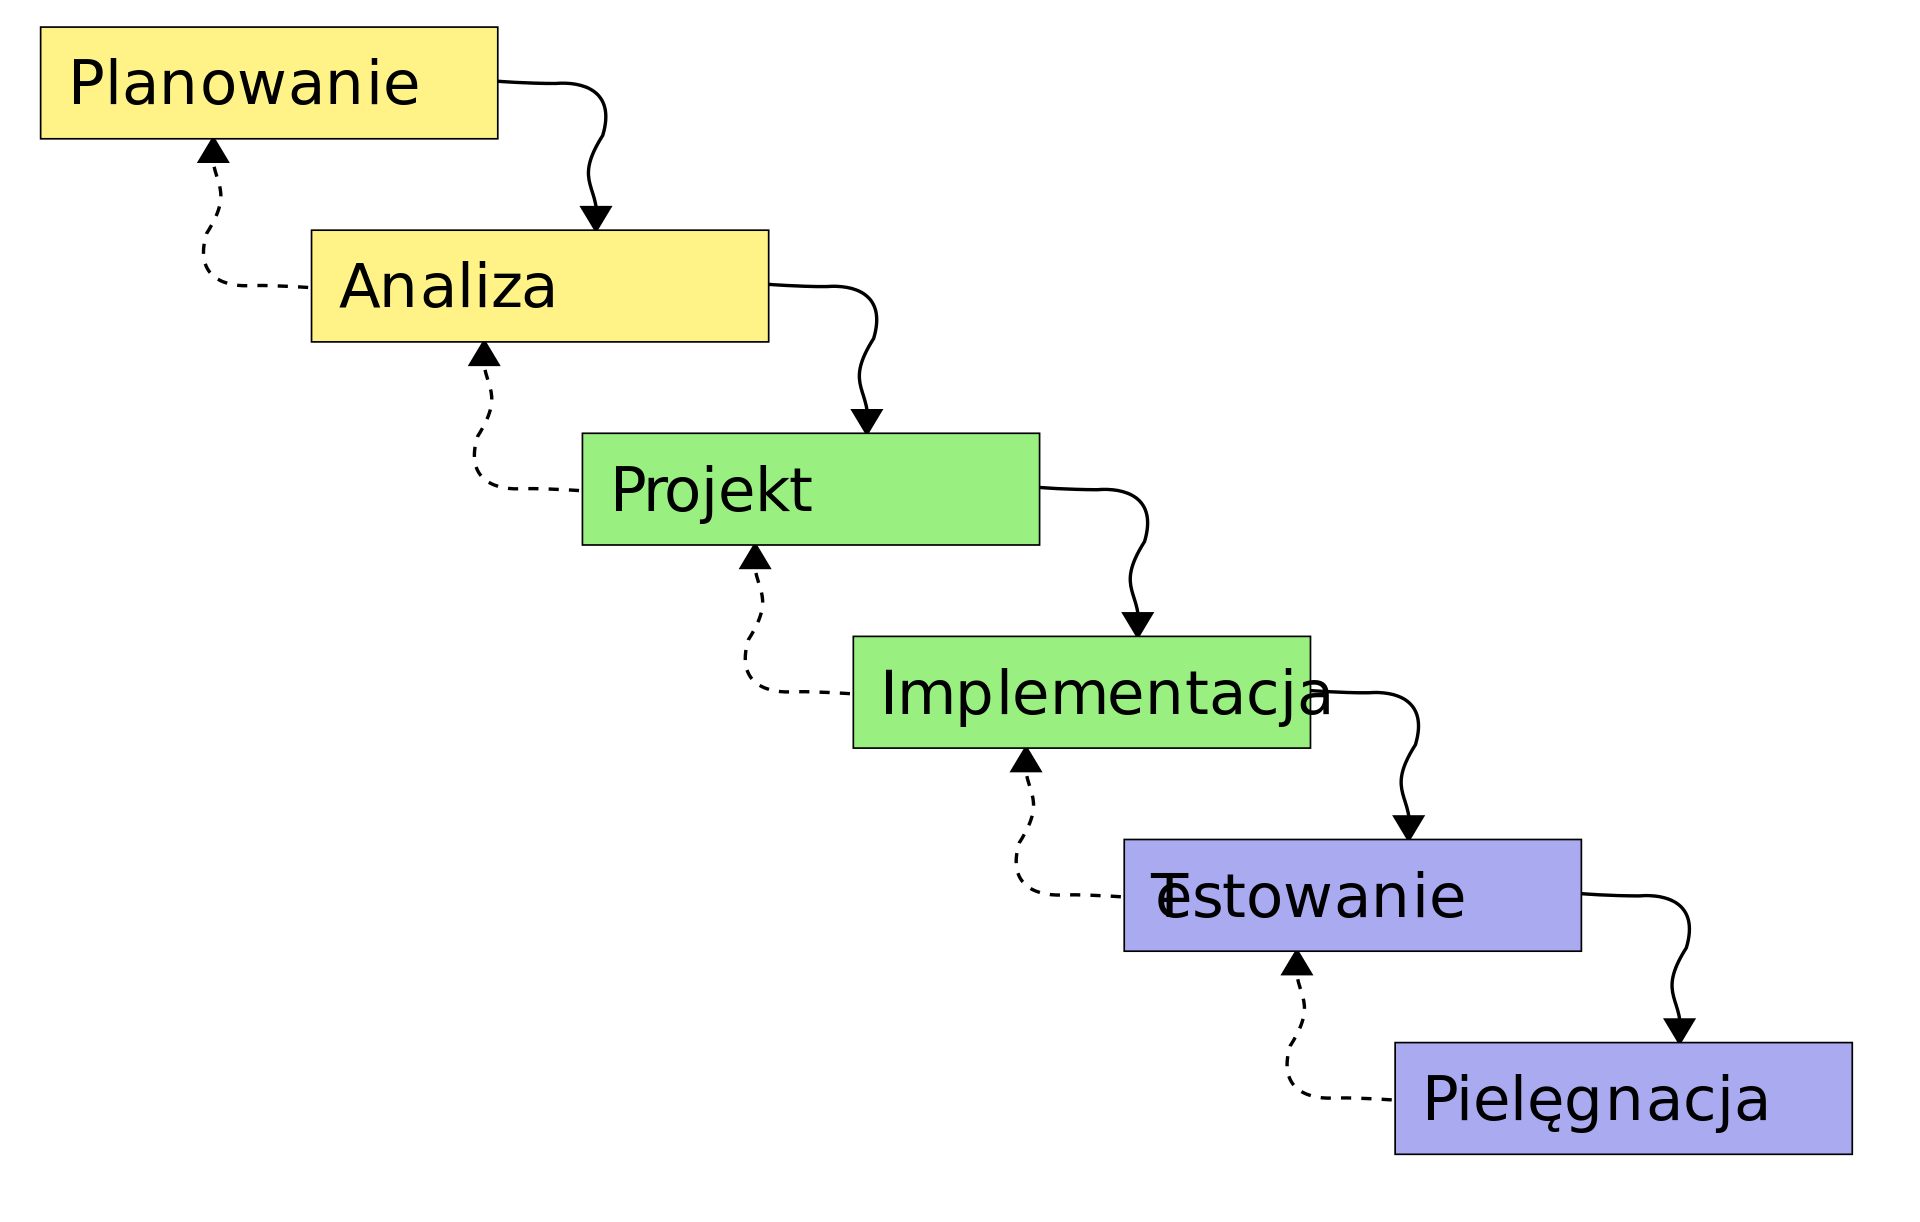
\includegraphics[width=10cm]{waterfall.png}
    \caption{Metodologia Waterfall}
    \label{fig:waterfall}
\end{figure}
Poszczególne etapy projektowe były wykonywane tylko raz podczas procesu tworzenia oprogramowania. Z tego faktu wszelakie zmiany na późniejszym etapie projektowym były trudne w realizacji. Konkurencja na rynku oprogramowania komputerowego była na tyle niewielka, że producenci oprogramowania nie musieli przejmować się zanadto uwagami od użytkowników - to sprawiało, że Waterfall spełniał swoje zadania. 
\par
Pierwsze dziesięciolecie XXI wieku spopularyzowało jedno z największych osiągnięć ludzkości - Internet. Nowa rzeczywistość w której ludzkość coraz więcej czasu spędza przed urządzeniami elektronicznymi postawiła przez twórcami oprogramowania nowe wymagania. Dodatkowo coraz większe grono przedsiębiorców zaczyna dostrzegać w produkcji oprogramowania zyski. Użytkownicy zaczynają coraz bardziej spoglądać na przyjemny dla oka wygląd oprogramowania oraz jego prostotę. Metodyka zaproponowana przez autorów manifestu Agile zdaje się świetnie wpisywać w wizję tworzenia oprogramowania na miarę nowego tysiąclecia.
\par
Jedną z bardziej znanych implementacji Agile jest metodologia o nazwie Scrum.
\begin{figure}[htbp]
    \centering
    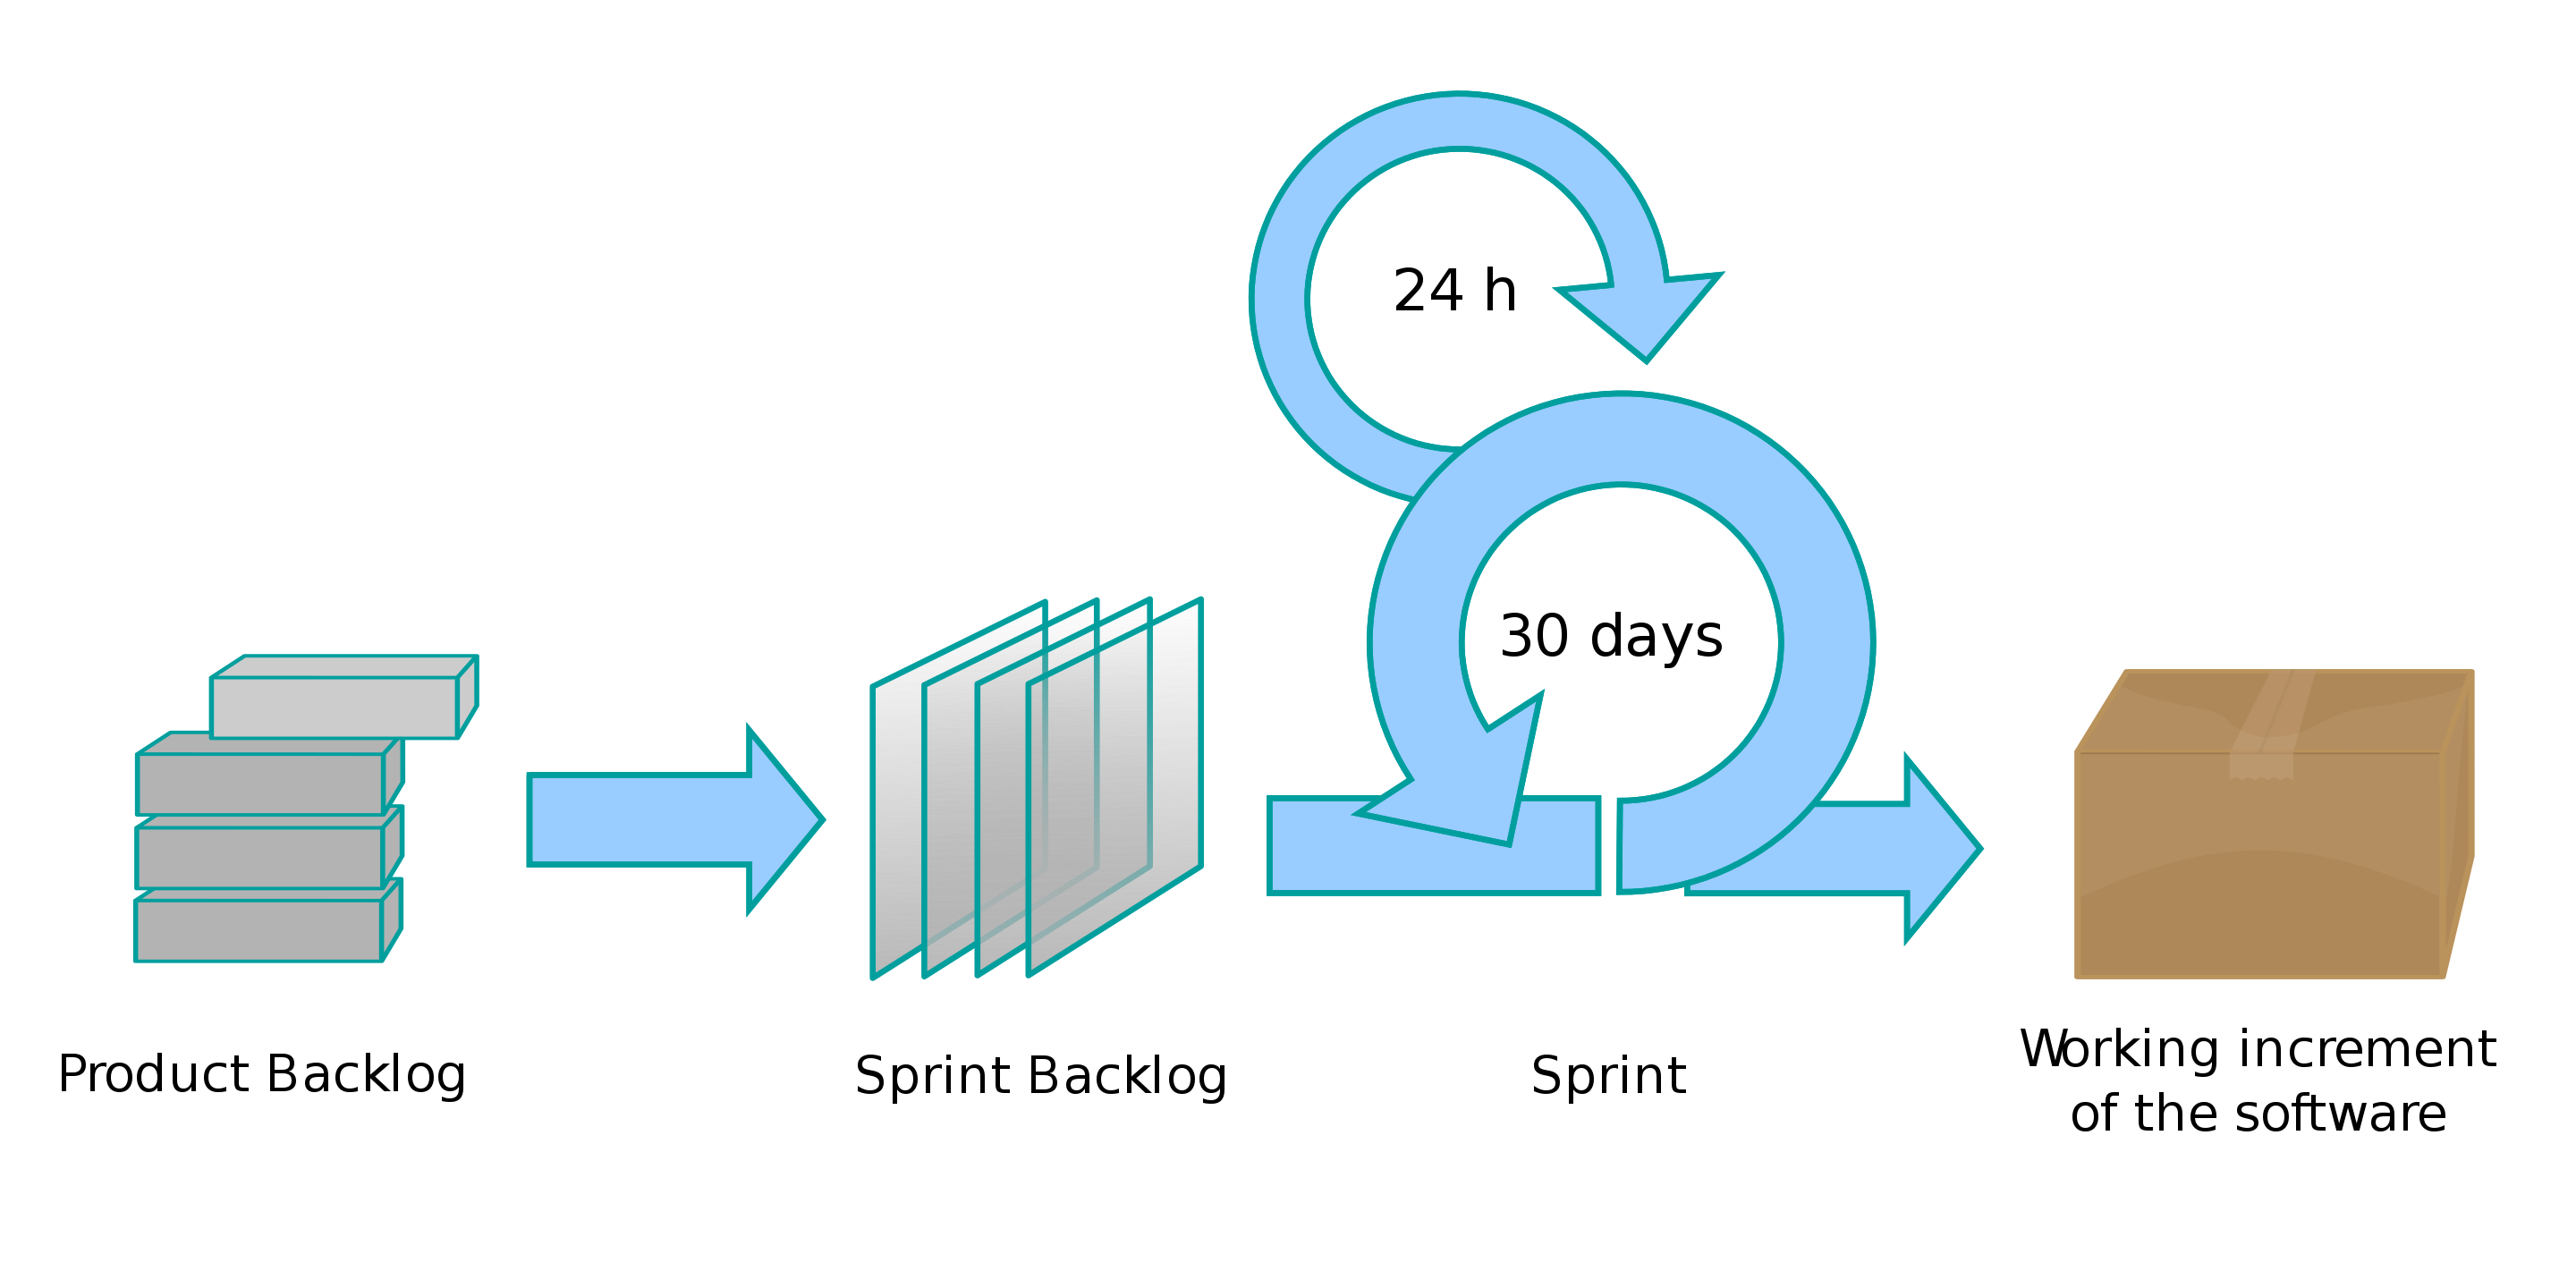
\includegraphics[width=10cm]{scrum.png}
    \caption{Framework Scrum}
    \label{fig:scrum}
\end{figure}
Zakłada się w niej, że oprogramowanie powstaje w procesie kolejnych inkrementacji. Każda iteracja jest nazywana sprintem. Sprint ma z góry zdefiniowane ramy czasowe w których będzie on trwał. Na podstawie różnych czynników biznesowych opiekun projektu decyduje które zadania powinny trafić do danego sprintu, a które są mniej priorytetowe i mogą pozostać w tzw. backlogu. Efektem końcowym danego sprintu jest działający produkt, który jest wzbogacony o rzeczy dodane podczas trwania sprintu. Scrum sam w sobie nie narzuca, ile powinien trwać dany sprint, czy też jaki system powinien być stosowany do śledzenia zadań. Wszystko zależy od preferencji danego zespołu programistycznego. Integralną częścią każdego sprintu jest retrospektywa. Na takim spotkaniu zespół dyskutuje jakie zmiany należy dokonać w procesie, by uefektywnić pracę. Dzięki elastycznemu podejściu i możliwości ulepszania procesu Scrum wydaje się być dobrym rozwiązaniem dla zespołów, które wypuszczają oprogramowanie regularnie oraz zmieniają je na podstawie opinii użytkowników.
\subsection{Agile a automatyzacja}
Spełnienie wymagań wymienionych w manifeście Agile wydaje się być trudne w kontekście częstego wypuszczania działającej wersji. Oczekuje się tego, aby zespół deweloperski regularnie publikował działającą wersję podglądową oprogramowania dla osób nietechnicznych. Problem ten można rozwiązać na co najmniej dwa sposoby:
\begin{itemize}
    \item Manualny - Członek zespołu deweloperskiego regularnie według wymagań zajmuje się budowaniem wersji podglądowej oraz udostępnia ją osobom zainteresowanym,
    \item Automatyczny - Zespół deweloperski ustawia automatyczne procesy, które na serwerze budującym tworzą wersję podglądową aplikacji oraz publikują ją dla osób zainteresowanych.
\end{itemize}
Proces automatyczny jest preferowanym sposobem publikacji oprogramowania. Ma on kilka zalet nad sposobem manualnym. Nie tracimy czasu specjalisty, który musiałby poświęcić go na zbudowanie i publikację aplikacji. Drugą zaletą jest fakt, że serwer za każdym razem robi te same kroki podczas procesu budowania. Tym sposobem wykluczamy możliwość popełnienia błędu przez człowieka.
\par
Dobre praktyki związane z częstym budowaniem podglądowej wersji oprogramowania są określane jako DevOps. Len Bass, Ingo Weber oraz Liming Zhu w swojej książce \cite{DevOpsBook} określają DevOps jako zbiór praktyk których celem jest zmniejszenie czasu publikacji zmian na serwerze produkcyjnym przy jednoczesnej trosce o wysoką jakość. W praktyce często członkiem zespołu deweloperskiego jest tzw. DevOps. Jego zadaniem jest automatyzacja wszelakich procesów oraz często także utrzymanie środowiska produkcyjnego. Osoba na tym stanowisku powinna się cechować dobrą znajomością systemu operacyjnego, który jest używany na serwerach produkcyjnych oraz deweloperskich. Ponadto powinna być zorientowana w różnych rozwiązaniach chmurowych które współcześnie są coraz częściej używane.
\subsection{Git - kamień milowy dla deweloperów}
Ciężko byłoby sobie wyobrazić obraz dzisiejszego przemysłu IT, gdyby nie system kontroli wersji Git. Jego autorem jest Linus Torvalds. Co ciekawe stworzył on Git'a jako dodatkowy projekt, który miał pomóc w pisaniu jądra Linuxa. Dzięki Git'owi każdy członek zespołu deweloperskiego ma dostęp do wspólnego repozytorium, gdzie każdy może publikować swoje zmiany. Jedną z ważniejszych funkcji Git'a jest możliwość tworzenia własnych rozgałęzień kodu, gdzie dany programista wysyła swoje zmiany. Dalej w procesie merge'owania jest możliwe połączenie zmian danego dewelopera z kodem innych programistów. Dzięki tej cesze Git nadaje się świetnie do wszelakich projektów programistycznych, w których pracuje kilku programistów równolegle. Z biegiem lat Git stał się standardem.
\par
Powszechnie znaną dobrą techniką związaną z strukturą tego, co mamy na Gicie jest tzw. \textit{Git Workflow}. Wzorzec ten sugeruje, by używać 2 głównych gałęzi. Jedną, która będzie odzwierciedlała finalną, zdatną do użytku wersję oraz drugą, gdzie znajduje się wersja deweloperska. Pośrednie gałęzie służą do implementacji poszczególnych nowych funkcjonalności oraz do synchronizacji wersji deweloperskiej z gałęzią produkcyjną. Dzięki takiemu podejściu proces deployment'u na środowisko produkcyjne oraz testowe staje się o wiele prostszy, ponieważ mamy dwie gałęzie, które odzwierciedlają te środowiska. Na rysunku \ref{fig:git} możemy podejrzeć szczegółowy schemat, jak powinno wyglądać repozytorium Git'owe korzystające z wzorca \textit{Git Workflow}
\begin{figure}[htbp]
    \centering
    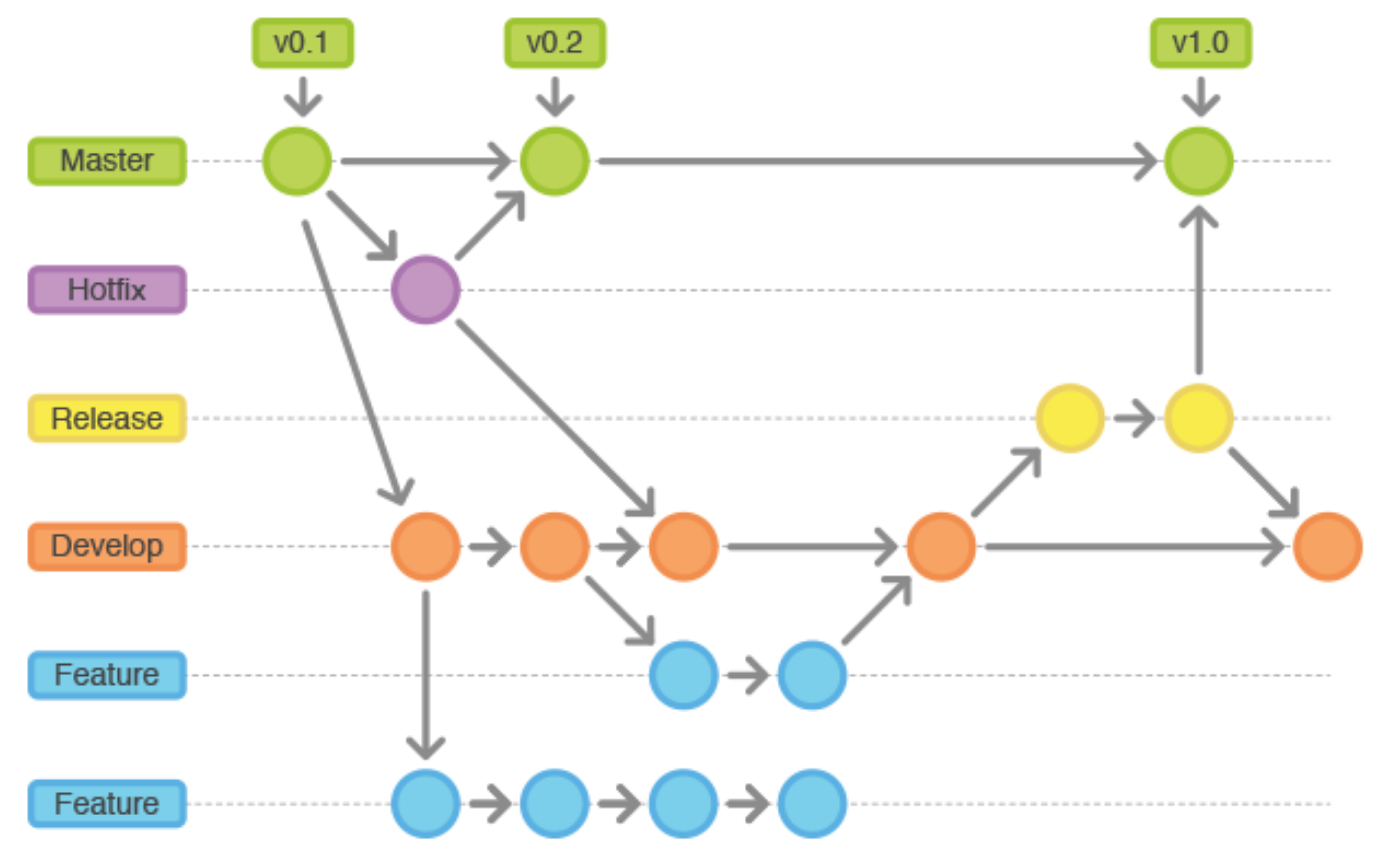
\includegraphics[width=10cm]{git.png}
    \caption{Git Workflow}
    \label{fig:git}
\end{figure}
\par
W pierwszym dziesięcioleciu XXI wieku popularne stały się rozwiązania SaaS (z ang. \textit{oprogramowanie jako usługa}) takie jak GitHub, GitLab czy też BitBucket. Dzięki takiemu rozwiązaniu nie musimy się przejmować utrzymaniem własnego serwera Git. Dodatkowo platformy SaaS zapewniają nam wszelakie aktualizacje, które usprawniają system. Platformy takie jak GitHub zapewniają narzędzia, które ułatwiają proces tworzenia oprogramowania. Narzędzia te są dopasowane, aby działać dobrze z naszym repozytorium. Przykładem takiego rozwiązania jest \textit{GitHub Pages}. Technologia ta pozwala publikować stronę www na podstawie plików, które są częścią repozytorium. Użytkownik definiuje, na której gałęzi oraz w którym folderze znajdują się pliki ze stroną internetową. Od tego momentu GitHub automatycznie stwarza nam stronę internetową dostępną pod subdomeną \textit{nazwauzytkownika.github.io}.
\subsection{Ciągła integracja}
Programiści podczas tworzenia nowych funkcjonalności powinni się upewnić, że ich zmiany nie zepsują tego, co już istnieje. Jednym z takich sposobów jest odpalenie testów. Najbardziej znanymi typami testów są:
\begin{itemize}
    \item testy jednostkowe - testy te skupiają się na testowaniu funkcji oraz klas w danym projekcie. Są najprostszą formą testowania podczas której zastępuje się wszelkie trzecie zależności tzw. \textit{mock'ami},
    \item testy integracyjne - są to testy, w których odpalany jest testowany projekt oraz wybrany projekt trzeci, z którym chcemy sprawdzić poprawność działania,
    \item testy e2e - testy te wymagają działającej w pełni aplikacji wraz z wszystkimi zależnymi projektami. Zazwyczaj sprawdzają najbardziej znaczące funkcjonalności naszej aplikacji.
\end{itemize}
Pisanie testów jest integralną częścią pracy programisty. Ich jakość oraz ilość jest znaczącym wskaźnikiem mówiącym o stanie danego projektu. Pozwalają one na tworzenie oprogramowania, które powinno mieć mniej błędów. Ciągła integracja przenosi odpowiedzialność za odpalanie testów z programisty na serwer ciągłej integracji.
\par
Testy to nie jedyna rzecz, która może być sprawdzana za pomocą ciągłej integracji. W procesie tym jest ważne, by zweryfikować jakość nowego kodu stworzonego przez developera. Przykładowymi rzeczami, które możemy zrobić podczas procesu ciągłej integracji jest:
\begin{itemize}
    \item sprawdzenie procentowego pokrycia testami projektu. Możemy na tej podstawie nie pozwolić na zmergowanie zmian, jeżeli przekroczymy z góry ustaloną procentową ilość kodu, która nie jest pokryta testami,
    \item sprawdzenie czy kod jest poprawnie sformatowany według ustalonych reguł. Proces ten nazywa się powszechnie \textit{lintowaniem}. Dzięki temu unikniemy problemu, w którym kod będzie różnie sformatowany w zależności dewelopera piszącego kod,
    \item testowanie aplikacji na niestandardowych systemach operacyjnych. Dzięki temu możemy się upewnić, że nasza aplikacja zadziała na mniej standardowych konfiguracjach. Jest to szczególnie istotne, jeżeli deweloperzy oraz testerzy nie skupiają się na testowaniu na danym systemie operacyjnym,
    \item sprawdzanie czy zależności trzecie, które są używane w projekcie nie mają żadnych podatności związanych z bezpieczeństwem aplikacji. Z racji tego możemy na wczesnym etapie wychwycić takie problemy i odpowiednio szybko zaaktualizować te biblioteki,
    \item zbudowanie obrazów dockerowych. Taki krok pozwala osobom znającym dockera bezproblemowe przetestowanie każdej gałęzi w naszym projekcie.
\end{itemize}
Dobór rzeczy, które chcemy zautomatyzować zależy od indywidualnych potrzeb danego projektu. Za duża komplikacja procesu ciągłej integracji może przynieść więcej szkody niż korzyści. Należy pamiętać, że programista musi czekać na to, aż proces ciągłej integracji się wykona.
Więcej o testach opisane jest w rozdziale 5.
\subsection{Ciągłe dostarczanie}
Podczas gdy ciągła integracja skupia się na upewnieniu, czy dane zmiany przechodzą testy, tak zadaniem procesów ciągłego dostarczania jest zbudowania aplikacji oraz umożliwienie jej późniejszej manualnej publikacji na środowisku produkcyjnym. Każdy projekt ma swoją własną specyfikę i proces ciągłego dostarczania jest inaczej ustawiany. Punktem wspólnym jest to, że człowiek decyduje, kiedy release'a oprogramowania powinien nastąpić.
\par
Zanalizujmy typowy przykład, jak może wyglądać proces ciągłej integracji. Mamy aplikację webową, która komunikuje się z bazą danych oraz wystawia API. Istnieją dwa środowiska gdzie działa ten serwis:
\begin{itemize}
    \item środowisko produkcyjne - jest to środowisko, które korzysta z produkcyjnej bazy i jest wykorzystywane przez klientów. Jest sprawą priorytetową, by środowisko to działało bez przestojów,
    \item środowisko staging'owe - środowisko to służy do testowania wersji deweloperskiej naszego serwisu. Możemy pozwolić sobie na to, by środowisko to miało przestoje od czasu do czasu.
\end{itemize}
Struktura gałęzi na Gicie jest prosta. Mamy dwa główne branche.
\begin{itemize}
    \item master - główna gałąź, gdzie jest trzymana najnowsza wersja stabilna serwisu,
    \item staging - gałąź deweloperska zawierająca zmiany, które nie były jeszcze dobrze przetestowane przez testerów.
\end{itemize}
\begin{figure}[htbp]
    \centering
    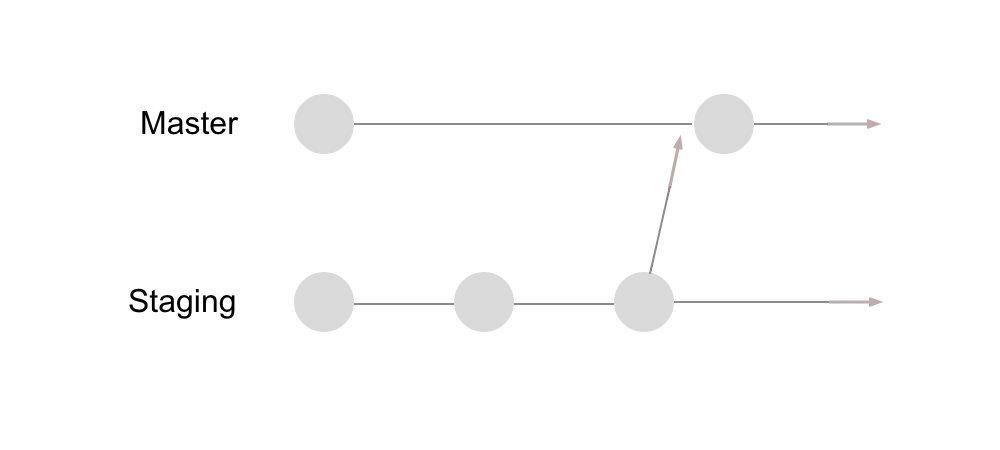
\includegraphics[width=10cm]{master-staging.png}
    \caption{Repozytorium z branchami master oraz staging}
    \label{fig:git}
\end{figure}
Struktura na Gicie dobrze odzwierciedla jakie środowiska mamy. Możemy wykorzystać ten fakt i za pomocą serwera ciągłego dostarczania budować aplikację i automatycznie ją instalować na serwerze stagin'owym za każdym razem, gdy ktoś zrobi commit'a na gałęzi staging. Dzięki takiemu podejściu oszczędzamy czas testerów. Nie muszą oni czekać na techniczną osobę, która zaktualizuje środowisko staging'owe. 
\par
By dalej ułatwić proces wypuszczania oprogramowania możemy zrobić podobne kroki jak przy staging'u dla wersji produkcyjnej. Za każdym razem, gdy ktoś wrzuca nowe zmiany na gałąź master możemy zbudować obraz (więcej o tworzeniu obrazów w rozdziale 2) z serwisem i wysłać go do rejestru obrazów. Tym sposobem kwestia wypuszczenia oprogramowania na serwer produkcyjny zostaje po stronie DevOps'a/administratora, który manualnie może wywołać proces aktualizacji danego serwisu. 
\subsection{Ciągła dystrybucja}
Ciągła dystrybucja jest rozszerzeniem ciągłego dostarczania. Proces ten zakłada, że zmiany, które znajdują się na naszej głównej gałęzi na repozytorium odzwierciedlają stan, który jest na serwerze produkcyjnym. Możemy to osiągnąć poprzez proces budujący aplikacje oraz aktualizujący serwer produkcyjny za każdym razem, gdy ktoś wrzuci nowego commit'a. Podejście to wymaga samodyscypliny i dobrej organizacji w zespole deweloperskim. Zespół musi być świadomy tego, że jeżeli dane zmiany nie są zanadto przetestowane, może to spowodować problemy na środowisku produkcyjnym, które jest kluczowe dla biznesu. W skrajnym przypadku może okazać się, że środowisko produkcyjne będzie działało z problemami przez dłuższy czas i dane, które trzymamy w bazie zostaną "zepsute" przez wadliwy kod.
\par
Problemy te możemy zminimalizować przez stosowanie następujących dobrych praktyk:
\begin{itemize}
    \item Wsteczna kompatybilność - jeżeli dana wersja ma w sobie błąd, administrator serwera w każdej chwili będzie w stanie cofnąć działającą wersję aplikacji do wersji, która nie miała problemów,
    \item Orkiestrator - nowoczesne orkiestratory takie jak np. Kubernetes (o orkiestratorach traktuje rozdział 2) umożliwiają zrobienie tzw. \textit{roll back}(cofnięcia do wcześniejszej wersji) w prosty sposób. Dzięki temu czas, w którym klienci doświadczyli problemów będzie stosunkowo krótki,
    \item Kopia zapasowa bazy danych - dzięki kopii możemy być pewni, że w przypadku "zepsucia" danych lub ich utraty przez błąd w programie będziemy w stanie je odzyskać,
    \item Testy e2e - dodanie testów całościowych systemu jest ważną rzeczą w kontekście ciągłej dystrybucji. Odpalając testy e2e na wersji deweloperskiej aplikacji możemy być bardziej pewni, że zmiany, które zostały dodane, nie psują istniejących funkcjonalności.
\end{itemize}
Dzięki wdrożeniu procesu ciągłej dystrybucji czas między stworzeniem danego kodu i wysłaniem go na repozytorium a uruchomieniem go na środowisku produkcyjnym zmniejsza się. Dodatkowo nie musimy poświęcać czasu administratora by zaktualizować środowisko produkcyjne. Należy pamiętać, że bez odpowiedniej dyscypliny programistów oraz braku stosowania dobrych praktyk proces ciągłej dystrybucji może spowodować więcej problemów niż korzyści. Zazwyczaj proces ten jest stosowany przez doświadczone zespoły deweloperskie.
\subsection{GitOps - czym jest?}
GitOps jest zbiorem dobrych praktyk, opisująca prawidłowy sposób wypuszczania aplikacji na środowisko deweloperskie jak i też produkcyjne. Jest to swoiste rozszerzenie procesu ciągłego dowożenia. Metodologia ta zachęca do trzymania plików konfiguracyjnych danego orkiestratora na repozytorium Git'owym. Dzięki takiej praktyce zyskujemy:
\begin{itemize}
    \item Możliwość weryfikacji jakości zmian, tzw. \textit{Code Review}. Dlatego że konfiguracja jest trzymana na Gicie, inni deweloperzy mogą ocenić, czy nasze zmiany są właściwe. Jest to dość duża zmiana względem tradycyjnego modelu, gdzie administrator sam decydował o zmianach w konfiguracji,
    \item Historię zmian - możemy dzięki temu przejrzeć, jak w przeszłości aplikacja była skonfigurowana,
    \item Przejrzystość systemu - każdy członek techniczny może podejrzeć to, w jaki sposób aplikacja działa na serwerze deweloperskim/produkcyjnym. W modelu tradycyjnym przeciętni członkowie nie wiedzą jak wygląda konfiguracja serwera - dostęp ma tylko administrator,
    \item Automatyzację procesu wypuszczania, czyli ciągłe dowożenie. Jeżeli projekt korzysta z praktyk GitOps, z definicji spełnia proces ciągłego dowożenia. Każda zmiana na gałęzi deweloperskiej/produkcyjnej powoduje to, że wypuszczamy nową wersję oprogramowania na serwerze.
\end{itemize}
\par
Termin GitOps został spopularyzowany przez orkiestrator Kubernetes. Pliki konfiguracyjne Kubernetesa są plikami w formacie YAML. Mocna decentralizacja sposobu, w jakim działa Kubernetes pozwala na trzymanie plików konfiguracyjnych pojedynczych jednostek logicznych w osobnych plikach. Jest to cecha ważna dla projektów opartych o architekturę mikroserwisową. W takich projektach mamy kilkanaście serwisów odpowiedzialnych za różne aspekty biznesowe aplikacji. Każdy taki serwis posiada własne repozytorium kodu w Gicie. Dzięki możliwości decentralizacji plików konfiguracyjnych Kubernetesa możemy dla każdego mikroserwisu trzymać te pliki osobno - każdy mikroserwis ma tylko pliki konfiguracyjne dotyczące samego siebie. Zapewnia to większą separację logiczną. Możność aplikowania na klaster Kubernetesowy pojedynczego pliku YAML, który stanowi tylko częściową konfigurację całego systemu, pozwala na aktualizację tylko pojedyńczego serwisu na klastrze. Dzięki temu poszczególne serwisy stają się bardziej niezależne od siebie.
\par
Załóżmy, że tworzymy aplikację opartą na mikroserwisach. Jednym z elementów tej aplikacji jest serwis zarządzający użytkownikami. Serwis ten zajmuje się logiką związaną z zarządzaniem użytkownikami. Jest on stworzony w języku JavaScript i swoją usługę wystawia na porcie 3000. Jego kod wygląda następująco:
\begin{lstlisting}[caption={Serwis zarządzający użytkownikami}]
    const express = require('express')
    const app = express()
    const port = 3000
    const users = [
        {
            name: 'Jan',
            email: 'jan@gmail.com',
        }, 
        {
            name: 'Kasia',
            email: 'kasia@gmail.com',
        }
    ]
    
    app.get('/get-all-users', (req, res) => {
        res.send(users)
    })
    
    app.listen(port, () => {
        console.log(`Users service listening at http://localhost:${port}`)
    })
\end{lstlisting}
Jednym z elementów tego serwisu jest plik konfiguracyjny Kubernetesa, który zajmuje się zdefiniowaniem usługi, jaki nasz serwis ma oferować. Usługa to jeden z obiektów Kubernetesa, który umożliwia przesłanie ruchu sieciowego do instancji z usługą. Plik konfiguracyjny wygląda następująco:
\begin{lstlisting}
kind: Service
apiVersion: v1
metadata:
  name: user-service
  namespace: production
  labels:
    run: user-service
  annotations:
    service.beta.kubernetes.io/aws-load-balancer-internal: 0.0.0.0/0
spec:
  selector:
    app: UserService
  ports:
  - protocol: TCP
    port: 80
    targetPort: 3000
  type: LoadBalancer
\end{lstlisting}
Okazuje się, że z jakiegoś powodu chcielibyśmy zmienić port, na którym nasz serwis z użytkownikami nasłuchuje. W tym celu musimy zmienić plik JavaScript'owy oraz plik YAML z konfiguracją Kubernetesa. Dzięki temu, że obydwa pliki są częścią jednego repozytorium możemy taką zmianę wykonać za pomocą jednego pull request'a. Nie musimy do całej akcji zmiany portu angażować administratora klastra Kubernetesowego - administrator jedyne przegląda, czy nasze zmiany są poprawne. Po zmergowaniu aktualizacja środowiska na klastrze następuje automatycznie. Przebiega to przy użyciu procesu ciągłego dowożenia.
\subsection{Serwery automatyzujące SaaS kontra self-hosted}
Wczesne lata rozwoju oprogramowania służącego do ciągłej integracji stały pod znakiem Jenkinsa. Jenkins to oprogramowanie, które jest zainstalowane na serwerze i pozwala tworzyć potoki automatyzujące. Może on służyć do stworzenia procesów ciągłej integracji, ciągłego dostarczania oraz ciągłego dowożenia. Jego charakterystyczną cechą jest to, że został on przygotowany do uruchomienia na własnym serwerze - tzw. self-hosted. Instalacja oraz utrzymanie Jenkinsa wymaga czasu specjalisty. Przewaga nad rozwiązaniami typu SaaS (z ang. \textit{oprogramowanie jako usługa}) jest taka, że mamy większą kontrolę nad tym jak Jenkins działa.
Jenkins to nie jedyne rozwiązanie self-hosted do automatyzacji:
\begin{itemize}
    \item CruiseControl - powstał w 2001 roku. Skupiał się na automatyzacji projektów tworzonych w języku Java,
    \item Hudson - prekursor Jenkinsa który zakończył swój żywot w 2015. Był tworzony jako alternatywa do CruiseControl. W roku 2011 został stworzony fork, którym teraz jest Jenkins,
    \item GitLab CI - jako jeden z nielicznych projektów oferuje możliwość wyboru i używania w formie self-hosted oraz w formie SaaS, dostępnej pod adresem \textit{gitlab.com}. Oprogramowanie to wyróżnia integracja z repozytorium kodu, dzięki której w kilku krokach możemy dodać automatyczne budowanie do naszego projektu. Kod całej platformy GitLab jest dostępny w formie open source.
\end{itemize}
\begin{figure}[htbp]
    \centering
    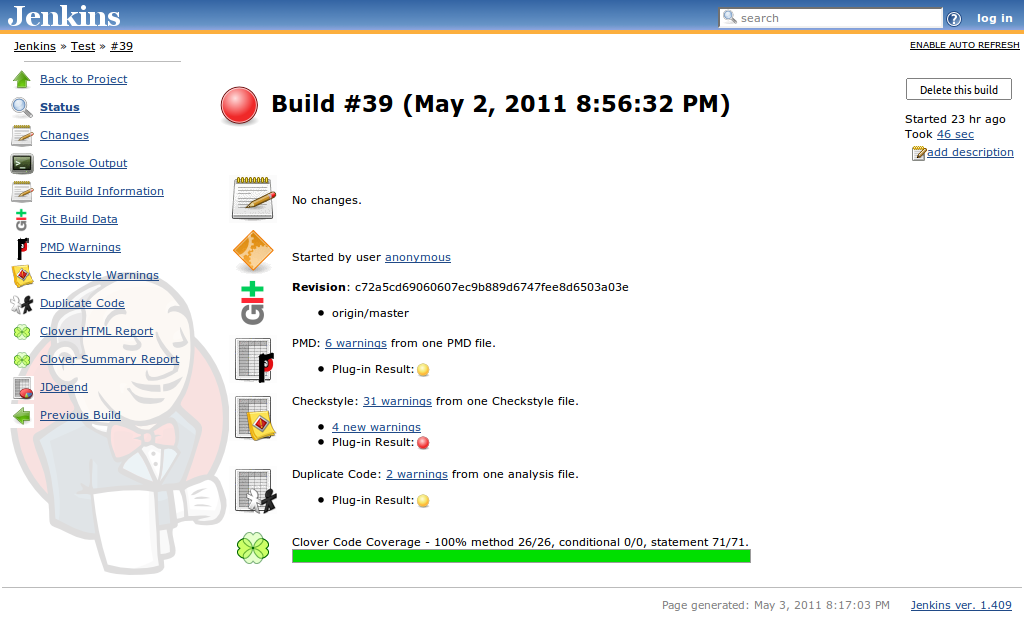
\includegraphics[width=12cm]{jenkins.png}
    \caption{Interfejs webowy Jenkinsa}
    \label{fig:jenkins}
\end{figure}
\par
Lata 10 XXI wieku przyczyniły się do popularyzacji rozwiązań typu SaaS, w których zespół deweloperski nie musi już utrzymywać własnego serwera z zainstalowanym tam oprogramowaniem. Dzięki SaaS utrzymaniem serwera zajmuje się strona trzecia, która za pewną opłatą zapewnia dostęp do aplikacji - zostawiając po swojej stronie sprawy związane z utrzymaniem oraz aktualizacją. Model ten stał się niezwykle popularny dla startup'ów. Firmy takie zazwyczaj posiadają tylko kilkoro ludzi technicznych. Użycie oprogramowania w formie SaaS pozwala takim zespołom skupić się na tworzeniu kodu, który ma dostarczać wartość biznesową. Do najpopularniejszych rozwiązań SaaS do automatyzacji należą:
\begin{itemize}
    \item Travis CI - jest to serwis który zapewnia integrację z repozytorium trzymanym na GitHubie oraz BitBuckecie. Jego kod jest oferowany w formie open source - aczkolwiek jego samodzielna instalacja na własnym serwerze jest dość wymagająca \cite{TravisCI},
    \item GitLab CI - może być używany w postaci SaaS. Oferuje on jedynie integrację z repozytorium hostowanym przez GitLaba,
    \item GitHub Actions - rozwiązanie do automatyzacji zaproponowane przez GitHuba. Zapewnia integrację z repozytorium kodu hostowanym na GitHubie. Jest zamknięto-źródłowym projektem,
    \item CircleCI - rozwiązanie podobne do Travis CI. Różnica polega na tym, że CircleCI zapewnia integrację tylko z repozytorium hostowanym na GitHubie. Dodatkowo jego kod nie jest dystrybuowany w formie open source - jest zamknięty.
\end{itemize}
\section{Wirtualizacja i orkiestracja}
% myślę, że opisanie tego jak wirtualizacja pomaga w CI/CD zasługuje na swój rozdział.
% Szczególnie mógłbym ten rozdział poświęcić dockerowi z faktu, że zdominował rynek.
% Warto tutaj byłoby napisać też o rozwiązaniach które były używane w przeszłości a zostały wyparte jak vagrant.
% Dodatkowo w rozdziale mozemy opisać na czym polega orkiestracja - Kubernates, docker swarm

\subsection{Wirtualizacja - początki}
Opisując automatyzację w procesów w przemyśle IT konieczne jest opisać wirtualizacje czyli kojelny kamień milowy w budowanie intrastruktury oraz współczesny sposob wytwarzania i dostarczania oprogramowania. Czym tak właściwie jest wirtualizacja? 
Żeby dobrze zrozumieć jak istotną role odgrywa wirtualizacja w automatyzacji warto spojrzeć wstecz i przyjrzeć się historii serverów i komputerów wogóle.   Jak podaje Paul E. Ceruzzi czyli autor książki "A History of Modern Computing", w przeszłości jeśli była potrzeba uruchomienia serwera, były zasadniczo dwie opcje: 
\begin{itemize}
    \item zbudować swój własny fizyczny serwer
    \item wynająć/kupić sprzęt komputerowy od firmy, która takie usługi prowadzi
\end{itemize}
W pierwszym przypaku budowanie własnego serwera wymaga duzej liczby inżynierów z odpowiednią wiedzą i doświadczeniem, narzędzi oraz materiałów do budowy. Niekażda firma będzie więc spełnić te wszystkie wymagania dlatego drugą opcją stała się więc zdecydowanie bardziej popularna. Pierwszą firmą która skorzystała na trudzie wykonania własnego serwera była firma IBM i tak w 1960 powstał IBM Mainframe, czyli sprzęt najwyższej klasy jak na uwczesne możliwości.

\begin{figure}[htbp]
    \centering
    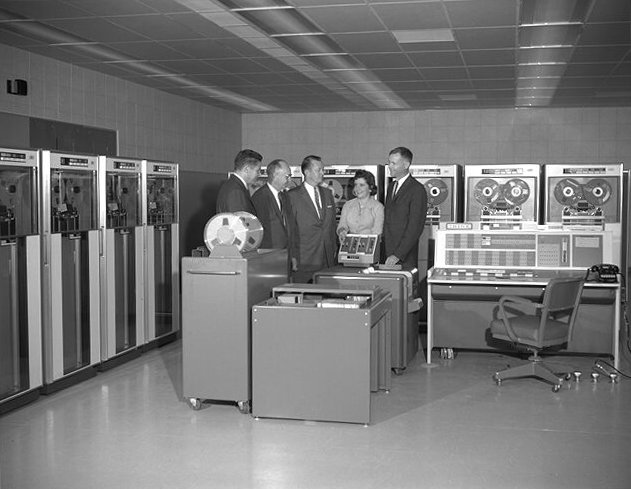
\includegraphics[width=10cm]{IBM-computer.jpg}
    \caption{IBM Mainframe}
    \label{fig:ibm-mainframe}
\end{figure}

Przez kolejne 20 lat sprzęty komupterowe firmy IBM dominowały rynek. Początkowo na Mainframie mozna było uruchomić tylko jedną aplikację do powodowało duze marnotratwo zasobów i czasu. Później została dodana wielozadaniowość co znacznie usprawniło działanie sprzętu. W 1980 roku był wielki "boom" technologiczny, który testował mozliwości serwera. Szybko się okazało, ze utrzymanie serwerów jest kosztowne. Konserwacja sprzetu, miejsce w którym serwery są przechowywane oraz koszty związane z administrowaniem sprawiły, ze na rynku pojawiła się potrzeba na technologie wirtualizacyjne i tak w latach 90 XX wieku w połączenie wydajnych procesów oraz znawców z dziedziny sprzętu komputerowego powstału wirtualne maszyny i wirtualizacja wogóle. 

\subsection{Czym są wirtualne maszyny?}
Wirtualne maszyny są kolejną warstwą abstrakci między urzytkownikiem a "metalem", czyli fizyczym sprzętem. Dzięki wykorzystnaiu tego mechanizmu, zamiast jednego systemu operacyjnego uruchomionego na komputerze, mozliwe jest uruchomienie wielu "gości" systemu operacyjnego na bazowym systemie operacyjnym. Dlaczego to jest takie przydatne? Teraz posiadając jedną mocną maszynę mozemy dowolnie dodawać i usuwać serwery. Tak wiec jeśli  teraz dodam dodatkową funkcjonalność do mojego programu, jedyne co muszę zrobić zeby go wdrozyć jest dodanie dodatkowej virtualnej maszyny jednym z serwerów, który ma wystarczająco duzo miejsca, żeby to zrobić. To rozwiązanie daje bardzo dużo elastycznosci. 
Jak dokładnie działa zarządzanie zasobami na wirtualnej maszynie?
Mechanizm dzięki któremu jest możliwa wirtualizacja nazywa się hypervisor. Hypervisor zarządza całym cyklem życia oraz funkcjonalnością wirtualnej maszyny. 
Do jego głównych zadań należą:
\begin{itemize}
    \item alokacja odpowiedinej ilości RAM'u, mocy obliczeniowej, pamięci dyskowej oraz zarządanie połączeniem z siecią
    \item startowanie wirtualnej maszyny 
    \item czyszczenie zasobów po zatrzymaniu wirtualnej maszyny
    \item zapewnianie izolacji dla odzielnie działających wirtualnych maszym 
    \item zarządzanie wirtualnymi maszynami
\end{itemize}
oraz wiele innych. 
Tak wiec podsumowując, jest jeden bazowy system operacyjny uruchomiony na komputerze, który udostępnia zasoby serwera wirtualnym maszynom i jeśli zasoby na tej wirtualnej maszynie się wyczerpią to nie ma to żadnego wpływu na inne wirtualne maszyny uruchomione na tym serwerze. Dodawtkowo pliki między wirtualnymi maszynami nie są współdzielone co sprawia, ze jeśli na jednej z wirtualnych maszyn zostanie usuchomiony niebezpieczny skrypt, szkody wyrządzone zostaną ograniczone do jednego systemu co sprawia, ze jest to rozwiązanie relatywnie bezpiecznie.
Wszystkie powyższe zalety nie są jednak "za darmo". Uruchamianie systemu operacyjnego wewnątrz innego systemu nie jest optymane jeśli chodzi o wydajność natomiast korzyści jakie niesie ze sobą wirtualizacja sprawiają, że jest ona wykorzystywana do dzisiaj w środowiach przemysłowych jak i naukowych. 
\subsection{Chmura publiczna}
W raz z rozwojem technologii rozwijali sie dostawcy chmury obliczeniowej tacy jak Microsoft Azure czy Amazon Web Services, u których mozna wynająć wirtualną maszynę. Maszyna ta będzie wyposazona w wstepnie przydzielona pamięcią ram oraz moca obliczeniowa (często moc obliczeniową nazywane są vitual cores bądź vCores). 
Zaletą tego podejścia jest brak konieczności utrzymywania serwerowni ale wciąż osoby wynajmujące odpowiedzialne są za utrzymanie oprogramowania które jest uruchamiane na serwerach. 
Dzięki chumurom możemy dynamicznie skalować nasze wirtualne maszyny, jedynym ograniczeniem są koszty jakie jesteśmy w stanie ponieść. Dostawaca jedynie dostarcza wirtualne maszyny, natomiast koniecznym wciąż jest zarządzanie całym oprogramowaniem, siecią, zaopatrzeniem, aktualizacją, itp. Wiele firm wciąż wybiera to rozwiązanie dlatgo powstały narzędzia jak Terraform, Chef, Puppet, Salt oraz wiele innych by ten proces maksymalnie uprościć. 
Podejściem tym jednak wciąż zgadzamy się na konsekwencje jakie niesie ze sobą uruchamianie jednego wystemu operacyjnego w drugim. Czy nie było by super gdybyśmy mogli wykorzystać system operacyjny hosta bez obawy, że marnujemy tak cenne zasoby naszego komputera? To właśnie było motywacją do powstania kontynerów czyli sposobu na budowanie infrastruktury dziś. 
\subsection{Kontynery}
Jak pewnie można sobie wyobrazić, kontynery dają nam wiele korzyści które niesie ze sobą wirtualna maszyna takie jak bezpieczeństwo oraz zarządzanie zasobami ale bez marnowania zasobów na system operacyjny. W kontynerach system operacyjny jest zastąpiony trzema możliwościami jakie daje linux: chroot, namespace oraz cgroup by oddzielić między sobą wrażliwe komponenty na naszej maszynie.
Żeby dobrze rozumieć czym jest kontyner oraz jak dużym krokiem na przód są dzisiejsze narzędzia do tworzenia kontynerów, w daleszej części pracy stworzę kontyner "ręcznie" wykorzystując wyżej wymienione filary kontynera. Wykonywane komendy będą uruchamiane na Ubuntu 18.04.3 LTS

\subsection{Chroot}
To jest linuksowa komenda, która pozwala zmienić bazowy katalog dla nowego processu. W tym ćwiczeniu ustawię bazowy katolog w wcześniej utworzony katalog co rozwiążemy problem bezpieczeństwa ponieważ processy na naszym kontynerze nie będą "widoczne" poza katalog bazowy. 
Aby zmienić katalog bazowy, stwórzmy wpierw nowy folder który będzie pełnił taką role "mkdir /my-new-root". Następnie przekopujmy podstawowe programy dostępne w systemie linux. "cp /bin/bash /bin/ls /my-new-root/bin/" oraz teraz musimy przekopiować biblioteki wykorzystując następujące kroki
\begin{lstlisting}
    - mkdir /my-new-root/lib{,64}
    - cp /lib/x86_64-linux-gnu/libtinfo.so.5 /lib/x86_64-linux-gnu/libdl.so.2 /lib/x86_64-linux-gnu/libc.so.6 /my-new-root/lib
    - cp /lib64/ld-linux-x86-64.so.2 /my-new-root/lib64
    - cp /lib/x86_64-linux-gnu/libselinux.so.1 /lib/x86_64-linux-gnu/libpcre.so.3 /lib/x86_64-linux-gnu/libpthread.so.0 /my-new-root/lib
\end{lstlisting}
Jeśli te kroki poprawnie wykonamy powinniśmy być wstanie urzyć komendy chroot /my-new-root bash oraz ls. W ten właśnie sposów zmieniamy katalog bazowy. 
\subsection{Namespaces}
Dzięki chroot sprawiliśmy, że dostęp do plików hosta z nowego kontynera będzie niemożliwy ale wciąż możemy ubić proces, zniszczyć system plików bądź nawet przechwytywać processy. 
Dzięki namespacom mamy możliwość "chowania" processów przed innymi processami. 
Zróbmy więc nasz nowy kontyner bardziej bezpiecznym. W tym celu posłużymy się komendą 'unshare', która uwtorzy nowy wyizolowany namespace z manespacu rodzica.

\begin{lstlisting}
    # instalowanie bootstarapa
    apt-get update -y
    apt-get install debootstrap -y
    debootstrap --variant=minbase bionic /better-root

    # zmiana namespace'a
    unshare --mount --uts --ipc --net --pid --fork --user --map-root-user chroot /better-root bash # this also chroot's for us
    mount -t proc none /proc # process namespace
    mount -t sysfs none /sys # filesystem
    mount -t tmpfs none /tmp # filesystem
\end{lstlisting}
powyższe komendy utorzą nowe środowisko z odizolowanymi processami, dyskami oraz siecią. Teraz nasz nowy kontyner juz nie widzi żadnych processów!
\subsection{cgroups}
W tym momencie mamy zabezmieczenie przed bałagnem w strukturze plików, processy się zgadzają ale co z zasobami? czy nie będzie tak, że jeśli wyczermie się załóżmy pamieć na jednym kontynerze to wszystkie inne przestaną działać? Na ten moment tak właśnie będzie i tu z pomocą przychodzą nam kontrol grupy (cgroups). Mechanizm ten polega na przydzielaniu zasobów hosta do jego dzieci na zasadzie jesli przekroczysz limit to koniec więcej nie będzie. 

Tutaj w jaki sposów wykorzystałem cgrupy w naszym kontynerze: 

\begin{lstlisting}
    apt-get install -y cgroup-tools htop
    cgcreate -g cpu,memory,blkio,devices,freezer:/sandbox
    ps aux 
    cgclassify -g cpu,memory,blkio,devices,freezer:sandbox <PID>

    cat /sys/fs/cgroup/cpu/sandbox/tasks
    cat /sys/fs/cgroup/cpu/sandbox/cpu.shares

    cgset -r cpu.cfs_period_us=100000 -r cpu.cfs_quota_us=$[ 5000 * $(getconf _NPROCESSORS_ONLN) ] sandbox

    cgset -r memory.limit_in_bytes=80M sandbox
    cgget -r memory.stat sandbox

    htop # will allow us to see resources being used with a nice visualizer

    yes > /dev/null # this will instantly consume one core's worth of CPU power
    yes | tr \\n x | head -c 1048576000 | grep n # this will ramp up to consume ~1GB of RAM
\end{lstlisting}
na ten moment mamy stworzony kontyner w najprostrzej postaci a pomimo, że nie poruszyliśmy niezwykle istotynych aspektów jak networking, deploying i building. 
Jak można zauważyć pisanie wszystkiego ręcznie nie jest trywialnym zadaniem. Dlatego na rynku pojawiłi się rozwiązania jak Docker do tworzenia, aktualizacji, zarządzania uruchomionymi kontynerami. Dzięki tego typu rozwiązaniom wykorzytanie kontynerów stało sie bardzo popularne nie tyklo w środowisku administratorów systemów ale również wsród programistów. 
\subsection{Obraz Dockera}
Jak podaje James Turnbull w swojej książce "The Docker Book: Containerization Is the New Virtualization", Obraz Dockera jest to plik złożony z kilku warst, który jest używany do wykonywania kodu w kontynerze. Jak pisze James, obraz jest zasadniczo zbudowany na podstawie instrukcji dla kompletnej i wykonywalnej wersji aplikacji, która opiera się na jądrze systemu operacyjnego hosta. Kiedy użytkownik Docker uruchamia obraz, może on stać się jedną lub wieloma instancjami tego kontenera.
\subsection{Obraz Dockera bez Dockera}
\begin{lstlisting}
    # uruchomienie kontynera Dockera z uruchomionym dockerem polaczonym do docker deamona
    docker run -ti -v /var/run/docker.sock:/var/run/docker.sock --privileged --rm --name docker-host docker:18.06.1-ce

    # uruchamianie kontynera apline 
    docker run --rm -dit --name my-alpine alpine:3.10 sh

    # eksportowanie systemu plikow kontynera
    docker export -o dockercontainer.tar my-alpine

    # stworzenie katalogu container-root oraz wypakowanie zawartosci dockercontainer.tar do tego katalogu
    mkdir container-root
    tar xf dockercontainer.tar -C container-root/

    # przypisanie przestrzeni nazw
    unshare --mount --uts --ipc --net --pid --fork --user --map-root-user chroot $PWD/container-root ash 
    mount -t proc none /proc
    mount -t sysfs none /sys
    mount -t tmpfs none /tmp

\end{lstlisting}

\subsection{Docker Image z Dockerem}
docker run -it alpine:3.10

Przykład ten dobrze ilustruje jak ważną rolę w procesie automatyzacji budowy kontynerów odgrywa Docker.
Docker oczywiście nie jest jedynym rozwiązaniem usprawniającym działanie kontynerów. Na rynku istnieją również takie rozwiązania jak Vagrant, Wox, Apache Mesos, LXC Linux Container oraz wiele inncyh. Każde rozwiązanie jest różne ale koncept pozostaje ten sam. Większość rynek jednak na moment korzysta z rozwiązania firmy Docker Inc. czyli Docker.


\subsection{orchestracja}

Kontenery same w sobie są przydatne w wielu, często wykorzystywanych przypadkach, takich jak aplikacje produkcyjne, uczenie się maszyn, tworzenie środowisk, środowisk programistycznych i jednorazowych eksperymentów. Orchestracja jak podaje Brendan Burns w książce "Designing Distributed Systems" odnosi się do automatycznego rozmieszczania, koordynacji i zarządzania konenerami z oprogramowaniem. Załóżmy, że budujemy aplikację zbudowaną z wielu mikroserwisów. Zarządzanie wielką architekturą wiąże się z koninecznością implementqcji takich rzeczy jak:
\begin{itemize}
    \item automatyczne skalowanie kontenerów i ich hostów
    \item automatyncze restartowanie kontenerów i ich hostów
    \item automatyczne naprawianie kontenerów i ich hostów
    \item balansowanie obciążeniem 
    \item znajdowanie nowo powstałych podów serwisów 
    \item wdrażanie zmian w kodzie serwisu bez przerywania jego działania 
    \item sprawdzanie czy pody poprawnie działają
    \item zarządzanie wrażliwymi danymi
    \item zarządzanie konfiguracją aplikacji
    \item komunikacja z bazą danych
    \item inne
\end{itemize}
Jak widać sporo kodu musiało bby zostać napisane, żeby wszystkie te rzeczy zaimplementować. Tu z ratukiem przychodzą narzędzia do orchestracji kontenerami ponieważ często oferują one rozwiązania na większość z tych problemów. Na czas pisanie tej pracy na rynku dominują trzy rozwiązania: Kubernetes, AWS ECS oraz Docker Swarm. W dalszej części skupimy się na tym pierwszym czyli Kubernetesie, ponieważ ma on zdecydowanie największe społeczeństwo i w razie potrzeby najławiej jest znalęź szukane informacje.

\subsection{Kubernetes}

Kubernates (albo jak równie często spotykane k8s. Ósemka znajduje się w nazwie ze względu na taką ilość znaków między k i s w nazwie) podobnie jak Jenkins (który będzie przedniotem rozważań w następnym rozdziale) jest narzędziem open-source czyli każdy może zobaczyć jej kod źródłowy. Narzędzie to jest plaftormą zasadniczo oferującą rozwiązania do wszytkich wymienionych problemów, a ponadto jest można go użyć zarówno w chmurze, lokalnie na fizycznych serwerach oraz roziązaniach hybrydowych. Dodatkowo rozwiązanie jest podzielone na moduły i każdy z nich (automatyczne restary, automatyczne skalowanie i tym podobne) jest, opinią autorów tej pracy i nie tylko, bardzo dobrze zaimplementowany. 
Projekt został zapoczątkowany w 2014 roku przez Google i jest połączniem systemu zarządzania klastrem, który Google wykorzystuje wewnętrznie nazywanym Borg oraz pomysłami i najlepszymi praktykami społeczności.
Przejdźmy więc go głównych konceptów z którch składa się Kubernetes:
\begin{itemize}
    \item Master jest serwerem, który koordynuje wszystko inne. To jest mózg klastra. Warto dodać, że niektórzy dostawny chmury publicznej nie pobierają opłat za korzystanie z master serwera na ich infrastrukturze. 
    \item Node (nie mylić z Node.js) to serwery robocze, które faktycznie będą obsługiwać twoje kontenery. Jeden node może obsługiwać jeden lub wiele kontenerów. Jeśli implementowane jest na przykład uczenie maszynowe i jest potrzeba dużych, rozbudowanych serwerów, aby przejść przez naukę, może się zdarzyć tak, że node może uruchomić tylko jeden kontener. Jeśli natomiasz w klustrze znajdują się mniejsze serwisy node może trzymać większą licznę kontenerów.
    \item technicznie rzecz biorąc nody są jedynie docelowym sprzętem na, który wdrażamy nasz produkt. W rzeczy samej może to być wirtualna maszyna, kontener a nawet fizyczny serwer. 
    \item Pod - najmniejsza i najprostsza jednostka w modelu obiektowym Kubernetesa, którą można tworzyć lub wdrażać. Reprezentuje ona działający proces w klastrze. Może zawierać jeden lub wiele kontenerów.
    \item Serwis - jest to grupa podów składająca się na jeden backend. Pody sewisu często są skalowane w górę i w dół więc polegając na ip kontenera do komunikacji jest mało efektywne. Lepszym roziązaniem jest stały address do, którego docelowe serwisy zawsze mogą się odwoływać i w tym celu właśnie zostały wymyślone serwisy
    \item Deployment - koncept ten polega na definiowaniu stanu podów aplikacji i po zdefiniowaniu, Kubernetes "pracuje" by doprowadzić i utrzymać apliakcję w takim stanie.
\end{itemize}

Dodatkowo do komunikacji z obiektami kubernetesa dostępne jest narzędzie wiersza poleceń o nazwie kubectl. Dzięki niemu mamy możliwość kanipulwoać stanem naszego klastra zarówno lokalnie jak i w chmurze.
\section{Hudson oraz Jenkins - klasyczne narzędzia do CI/CD}
% tutaj mógłbym zamieścić trochę informacji historycznych jak język java zrewolucjonował inżynierię oprogramowania i dalej rozwinąć, że pokłosiem tego było powstanie Jenkinsa.
% Myślę, że mógłbym tutaj opisać najbardziej uniwersalne rzeczy które są w nim używane. Wydaje mi się że mógłbym poszukać alternatyw do Jenkinsa by rozszerzyć ten dział.
% Jako część tego rozdziału mógłbym zawrzeć problem gdzie konieczne jest użycie Jenkinsa i to byłoby zrobione jako część praktyczna.
% Wbrew pozorom do niektórych zastosować Jenkins nadal jest używany, np do środowisk gdzie QA musi odpalać                        

\subsection{Inżynieria oprogramowania}
Kolejny rozdział tej pracy inżynierksiej poświęcimy na opisanie aspektów automatyzacji w processach tworzenia oprogramowania. 
Jako wprowadzenie do tego działu kolejny raz chciałbym na podstawie książki "The Phoenix Project: A Novel about IT, DevOps, and Helping Your Business Win" autorstwa Gene Kim i Kevin Behr pokazać jak popularyzacja komputerów spowodowała potrzebe na nowe technologie. 
Z biegiem czasów gdy komputery stawały się coraz to bardziej popularne, coraz to wiecej aplikacji czy to desktopowych czy to webowych powstawało. Coraz to więcej programistów i aplikacji pojawiało się ma rynku. Powstawało wiele firm tworzących oprogramowanie i w związku z dużą konkurencyjnością, firmy wymyślały nowe sposoby poprawy wdrażania oprogramowania, sprawdzania jakości kodu, dostępności infrastruktury oraz poprawy wydajności kodu, po to by wyróżnić się na konkurencyjnym rynku. Coraz to większą rolę w środowisku IT zaczęli odgrywać  DevOpsi. Czyli jak podają autorzy książki, osoby tworzące równowagę pomiędzy działami wytwarzania oprogramowania i zarządzania systemami.  


\subsection{DevOps} 
Jak wspomina Gene i Kevin w swojej książce do głównych zadań inżynierów DevOps należą:
\begin{itemize}
    \item projektowanie strategi kontroli wersji
    \item wdrożenia i integracja kontroli źródeł
    \item implementacja i zarządzanie infrastrukturą build'owania
    \item wdrżanie przeływu kodu
    \item zarządzanie konfiguracją aplikacji i jej tajnymi danymi
\end{itemize}

Dawniej kiedy wszystkie te koncepty nie były jeszcze tak popularne jak dzisiaj, autorzy ksiązki opisują duży chaos w zarządzaniu kodem. Opisują środowiska przechowywania kodu jako miejsce mało zadbane i prowadzone bez głębszego pomysłu.

DevOps to podejście do rozwoju oprogramowania, które obejmuje ciągły rozwój, ciągłe testowanie, ciągłą integrację, ciągłe wdrażanie i ciągłe monitorowanie oprogramowania w całym cyklu jego życia. Jest to proces przyjęty przez wszystkie najlepsze firmy w celu opracowania wysokiej jakości oprogramowania i skrócenia cyklu życia produktu, co przekłada się na większą satysfakcję klientów, czego każda firma poszukuje.
Inżynierowie DevOps codziennie korzystają z wielu narzędzi jak Kibana czy Splunk do monitorowania aplikacji, Git czy Mercurial do zarządzania kodem, Puppet, Ansible bądź Chef do zarządzania konfiguracją i wiele innych. 
W dajszej częsci pracy skupimy się na narzędziu, które subiektywnym zdaniem autorów tej pracy najlepiej obrazuje codzienne zadania automatyzujące inżynierów DevOps czyli Jenkins.
Na potwierdzenie słuszności naszego wyboru warto dodać, że narzędzie to w 2011 roku wygrało nagrodę Bossie (Best of Open Source Software Award) oraz w 2014 prestiżową nagrodę Geek Choice.  

\subsection{Projekt}

Celem projektu jest przybliżenie możliwości automatyzacji na podsawie nowoczesnego narzędzia codziennie wykorzystywanego w świecie IT. Tym narzędziem bęzie Jenkins. 
Na potrzeby tego projektu stworzę również prostą aplikację Spring Boot, która będzie implementowała podstawowe założenia API RESTful. Jenkins oraz aplikacja w nawiązaniu do poprzedniego działu tej pracy będą uruchomione na kontynerach. Celem tego zabiegu jest zaprezentowanie działania tego narzędzia. 

\subsection{Jenkins}

Jest to projekt open sourcowy (co oznacza, że każdy może wprowadzać zmiany do projektu) napisany całkowicie w języku Java. Jenkins wykonuje szereg zadań by osiągnąć założenia ciągłej integracji poprzez automatyzację części związanych z budowaniem, testowaniem i wdrażaniem. To sprawia, że developerzy mogą ciągle pracować nad ulepszaniem produktu nad którym pracują. Ponaddto Jest to system, który działa na servletowych kontynerach jak na przykład Apache Tomcat. 
Jenkins automatyzuje budowanie aplikacji dzięki czemu developerzy są w stanie wcześnie wykrywać błedy w swoim kodzie. Do głównych zalet Jenkinsa zdecydowanie można zaliczyć społeczność, która się wokół Jenkinsa przez wiele lat działalności zbudowała. Jest to narzędzie nie tylko łatwo rozszerzalne ale również posiada wiele zaimplementowanych wtyczek. 
Kilka przykładów zastosowania tego oprogramowania:
\begin{itemize}
    \item budowanie aplikacji przy pomocy narzędzi do buildowania jak Gradle, Maven czy inne 
    \item automatyzacja testów  (Nose2, PyTest, Robot, Selenium i wiele innych)
    \item wykorzystywany do testowania skryptów (bash, bat, zsh, inne)
    \item raportowanie na przykłąd wyświetlanie wyników testów
\end{itemize}

Na czas pisania tej pracy Jenkins posiada ponad 1500 wtyczek stworzonych przez społeczność, dzięki którym doświadczenie z korzystania z narzędzia oraz aktywności związane z budowaniem, wdrażaniem i automatyzacją projektu stają się lepsze. 

\subsection{Historia}

Jenkins nie zawsze nosił nazwę taką jak dziś. Został stworzony przez pracownika Sun Microsystems Kohsuke Kawaguchi w lato 2004 roku a pierwsze wydanie nastąpiło w styczniu 2005 roku pod nazwą "Hudson". Oprogramowanie występuje pod nazwą Jenkins od 2011 roku po tym jak firma Sun Microsystems została wykupiona przez firmę Oracle. Na początku Hudson i Jenkins były tworzone osobno ale po przejęciu firmy zarząd postanowił połączyć oba projekty i zachować nazwę Jenkins, gdyż posiadał on znacząco wiekszą społeczność niż projekt Hudson. Dzisiaj wspieranie dla projektu Hudson nie jest oficialnie prowadzone. 

\subsection{Architectura}

Aby dobrze zrozumieć jak działa narzędzie w tym rozdziale opiszę co się stanie jeśli developer zapisze zmiany na repozytorium, przedstawię przykładową implementację metodologii ciągłej integracjii/ciągłego wdrażania w Jenkinsie oraz opiszę jak wygląda architektura Master-Slave.

Według Johna Smart, czyli autora książki "Jenkins: The Definitive Guide" istnieje kilka kroków, które opisują jak działa komunikacja między elementami w Jenkinsie: 
\begin{itemize}
    \item inżynier zmienia kod źródłowy aplikaji i zapisuje zmiany do reposytorium
    \item repozytorium jest regularnie sprawdzane przez serwer Jenkins CI i w razie jakiś zmian ten sam serwer pobiera je do dalszej pracy
    \item w następnym kroku jest sprawdzane czy zapisane zmiany "przechodzą". Build  jest wykonywany i jeśli nie było żadnych błędów generpwany jest plik wykonywalny. Jeśli pojawią się jakieś errory, tworzony jest email z linkiem do logów builda. 
    \item w przypaku gdy budil był udany, plik wykonywalny jest wdrażany na środowiku testowym. Ten krok ponaga zrealizować krok ciągłego testowania ponieważ plik wykonywalny przechodzi przez wiele testów automatycznych. Jeśli są problemy w którymś z testów programiści pównież są o tym informowani.
    \item jeśli nie ma problemów podczas buildu, integracji czy testowania zmiany są automatycznie wdrażane na środowisko produkcyjne
\end{itemize}



Często się zdarza, że pojedyńczy server może nie wystarczyć. Na przykład:
\begin{itemize}
    \item testy muszą być wykonane na różnych środowiskach
    \item pojedyńczy serwer nie jest wstanie obsłużyć ruchu, który jest wyagany w wielkich systemach.
\end{itemize}

W tych przypakach wykorzystywana jest Master-slave architektura wspomniana któtko na początku tego działu. Jak więc wygląda ta architektura? O tym właśnie będzie dalsza część tej pracy. 
A więc master-slave architektura jest używana do zarządzania rozszerzonymi buildami. Komuniakacja między serwerem mastera i slave'a odbywa się poprzez protokół TCP/IP. 

\subsection{Master}

To jest główny serwer Jenkinsa. Do jego głównych zadań należą:
\begin{itemize}
    \item zorganizowanie jobów builda
    \item wybór odpowiedniego slave'a
    \item monitorowanie czy, któryś ze slave'ow i włącznie/wyłącznie w zależności od potrzeby.
    \item reportowanie wyników builda do developerów
\end{itemize}

Master również może zostać wykorzystywany bezpośrednio do wykonywnia jobów ale rekomendowane jest, żeby zadania były one na slaveach wykonywane.

\subsection{Slave}

Slavemi nazywami zewnętrzną maszyne połączoną z Masterem. Zależnie od projektu oraz wymagań builda liczna slave'ow może się różnić. Slavy mogą być uruchomione na różnych systemach operacyjnych i zależnie od wymagań builda, master wybiera odpowiedniego slavea do wykonania builda i testów. 
Do głównych zadań slave'a należą:
\begin{itemize}
    \item nasłuchiwanie na polecenia Mastera
    \item wykonie jobów zleconych przez Mastera
    \item developerzy mogą "ręcznie" wybrać slave na którym ma zostać wykonane zadanie ale z reguły Master dobiera najbardziej pasujący slave'a.
\end{itemize}

\begin{figure}[htbp]
    \centering
    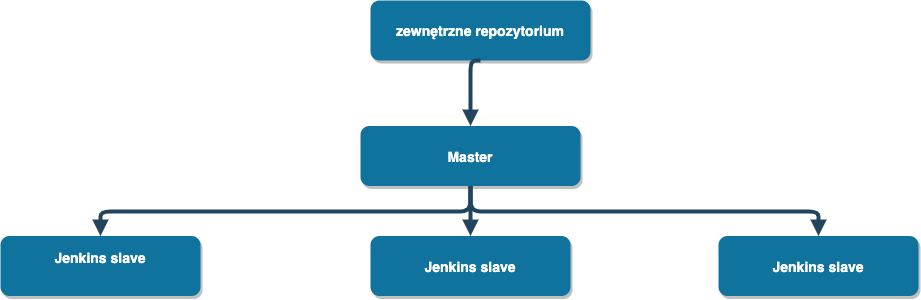
\includegraphics[width=10cm]{master-slave.png}
    \caption{master-slave architektura}
    \label{fig:master-slave}
\end{figure}

Jak do tej pory pokrótce opisaliśmy za co odpowiedzialne są poszczególne komponenty w Jenkinsie. Przedstawię teraz przykładową architekturę oraz opiszę za co są odpowiedzialne poszczególne jej elementy 

\begin{figure}[htbp]
    \centering
    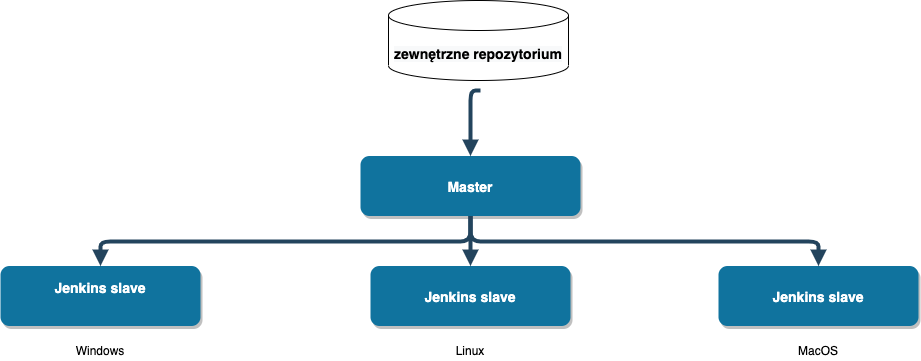
\includegraphics[width=10cm]{archritektura-przyklad.png}
    \caption{architektura przykład}
    \label{fig:jenkins-architektura}
\end{figure}

\begin{itemize}
    \item Developer zapisuje zmiany w kodzie na zewnętrznym repository
    \item master jest połaczony do repozytoriom i regularnie sprawdza czy pojawiły się jakieś zmiany. Wszysktie slavey są połączone z masterem.
    \item master otrzymuje żądanie wykonania zadania, które zostaje przekazane do odpowiedniego slavea. 
    \item slave wykonuje zlecone zadania, generuje raporty testów. Master ciągle monitoruje wyniki testów.
\end{itemize}

W dalszej części pracy zaprezentujemy przykładowe zastosowanie tego narzędzia. 

\subsection{Aplikacja}

Aplikacja implementuje REST api i będzie wyświetlała imię użytkownika podane do path URL. Projekt posiada proste pliki java w których jest umieszczona logika naszej aplikacji oraz pliki Maven'a do budowania naszej aplikacji. Tak oto wygląda kod pliku pom.xml 

\begin{verbatim}
    <?xml version="1.0" encoding="UTF-8"?>
<project xmlns="http://maven.apache.org/POM/4.0.0" xmlns:xsi="http://www.w3.org/2001/XMLSchema-instance"
	xsi:schemaLocation="http://maven.apache.org/POM/4.0.0 https://maven.apache.org/xsd/maven-4.0.0.xsd">
	<modelVersion>4.0.0</modelVersion>
	<parent>
		<groupId>org.springframework.boot</groupId>
		<artifactId>spring-boot-starter-parent</artifactId>
		<version>2.3.2.RELEASE</version>
		<relativePath/>
	</parent>
	<groupId>com.example</groupId>
	<artifactId>rest-service</artifactId>
	<version>0.0.1-SNAPSHOT</version>
	<name>rest-service</name>
	<description>Demo project for Spring Boot</description>

	<properties>
		<java.version>1.8</java.version>
	</properties>

	<dependencies>
		<dependency>
			<groupId>org.springframework.boot</groupId>
			<artifactId>spring-boot-starter-web</artifactId>
		</dependency>

		<dependency>
			<groupId>org.springframework.boot</groupId>
			<artifactId>spring-boot-starter-test</artifactId>
			<scope>test</scope>
			<exclusions>
				<exclusion>
					<groupId>org.junit.vintage</groupId>
					<artifactId>junit-vintage-engine</artifactId>
				</exclusion>
			</exclusions>
		</dependency>
	</dependencies>

	<build>
		<plugins>
			<plugin>
				<groupId>org.springframework.boot</groupId>
				<artifactId>spring-boot-maven-plugin</artifactId>
			</plugin>
		</plugins>
	</build>

</project>

\end{verbatim}

W pliku tym znajdują sie zależności jak i wtyczki Spring Boot potrzebne do działania naszej aplikacji. 

\subsection{Dockerfile} 

Dockerfile jest to specyficzny plik dzięki, któremu pozwala nam zdefiniować jak powinien nasz kontyner wyglądać. Każda linia w Dockerfilu to osobna instrukcja, która opisuje jak powinien wyglądać końcowy kontyner. 

Na początku konieczne jest zbudowanie naszego programu, żeby można było go wykorzystać w naszym dockerfilu. W tym celu użyję komendy ./mvnw clean package, która skompiluje nasz kod i spakuje go do pliku wykonywalnego rest-service-0.0.1-SNAPSHOT.jar. Plik ten będzie wykorzystywany w naszym Dockerfilu. 

\begin{lstlisting}
    FROM openjdk:8-jdk-alpine
    VOLUME /tmp
    ADD target/rest-service-0.0.1-SNAPSHOT.jar app.jar
    ENTRYPOINT ["java","-jar","app.jar"]
    EXPOSE 2222
\end{lstlisting}


Każda linia tego pliku dodaję dodatkową funkcjonalnnośc do naszego projektu wiec warto wyjaśnić co w każdej lini się znajduje. W pierwszej linii importujemy dostępny w oficialnym repozytorium Dockera linuxowy obraz alpine wraz z zainstalowanym na nim openjdk. Alpine Linux jest to podstawowy system operacyjny charakteryzujący się prostotą oraz małym rozmiarem pojemości dyskowej jaką zajmuje. Nie posiada on zbędnych bibliotek, które niepotrzebnie zajmowały by miejsce na naszym kontynerze stąd też nasz wybór padł właśnie na ten kontyner. Następnie dodajemy wcześniej spakowany plik jar, który znajduje się w folderze /target. Kolejno zaznaczamy jaka komenda powinna zostać uruchomiona po uruchomienu kontynera oraz udostępniamy port 2222 do dostępu publicznego. 
Kolejno w konsoli użyłem trzy komend by zbudować nasz projekt i uruchomić go w kontynerze. 
\begin{lstlisting}
    mvn clean install 
    docker build -t pracainzynierka
    docker run pracainzynierska -p 2222:2222
\end{lstlisting}
W pierwszej kolejności lokalnie budujemy projekt by zaktualizować nasz plik jar, ktory jest nam potrzebny podcza budownia obrazu Dockera w drugiej komendzie. W ostatnik kroku uruchamiamy nasz kontyner. Po tych krokach wchodząc pod adres http://127.0.0.1:2222/greeting otrzymamy powitalną odpowiedź z naszego kontynera. 
W dalszej części pracy inżynierksiej zautomatyzujemy ten proces przy pomocy Jenkinsa. 

\subsection{Automatyzacja przy użyciu Jenkinsa}

Jako, że użyliśmy dockera by uruchomić naszą aplikację lokalnie, nic nie szkodzi na przeszkodzie by również użyć Dockera do pracy z Jenkinsem. Problemem jaki napotkaliśmy podczas implementacji tego rozwiązania polegał na braku komend dockera wewnątrz kontynera dlatego trzeba było dodać kikla warstw do naszego Jenkinsowego Dockerfil'u by umożliwić taką funkcjonalność. 

finalna wersja pliku Dockera wygląda następująco: 

\begin{lstlisting}
    from jenkins/jenkins:lts
    USER root
    RUN apt-get update -qq \
    && apt-get install -qqy apt-transport-https ca-certificates curl gnupg2 software-properties-common
    RUN curl -fsSL https://download.docker.com/linux/debian/gpg | apt-key add -
    RUN add-apt-repository \
   "deb [arch=amd64] https://download.docker.com/linux/debian \
   $(lsb_release -cs) \
   stable"
    RUN apt-get update  -qq \
    && apt-get install docker-ce=17.12.1~ce-0~debian -y
    RUN usermod -aG docker jenkins
\end{lstlisting}

Kolejno przy użyciu druch kolejnych komend:
\begin{lstlisting}
    docker image build -t jenkins-docker .
    docker container run -d -p 8080:8080 -v /var/run/docker.sock:/var/run/docker.sock jenkins-docker
\end{lstlisting}

jesteśmy wstanie wchodząc pod localhost:8080 adress url finalnie dostać się do Jenkinsa

\subsection{Konfigurowanie Jenkinsa}

Głównymi narzędziami, które będzie trzeba skonfigurować jest JDK, Maven oraz GIT by móc budować aplikacje oraz klonować kod z repozytorium. Wszystkie kroki wykonuje się z poziomu Jenkinsa. W naszym projekcie konfiguracja wygląda jak na screenshotach poniżej:

\begin{figure}[htbp]
    \centering
    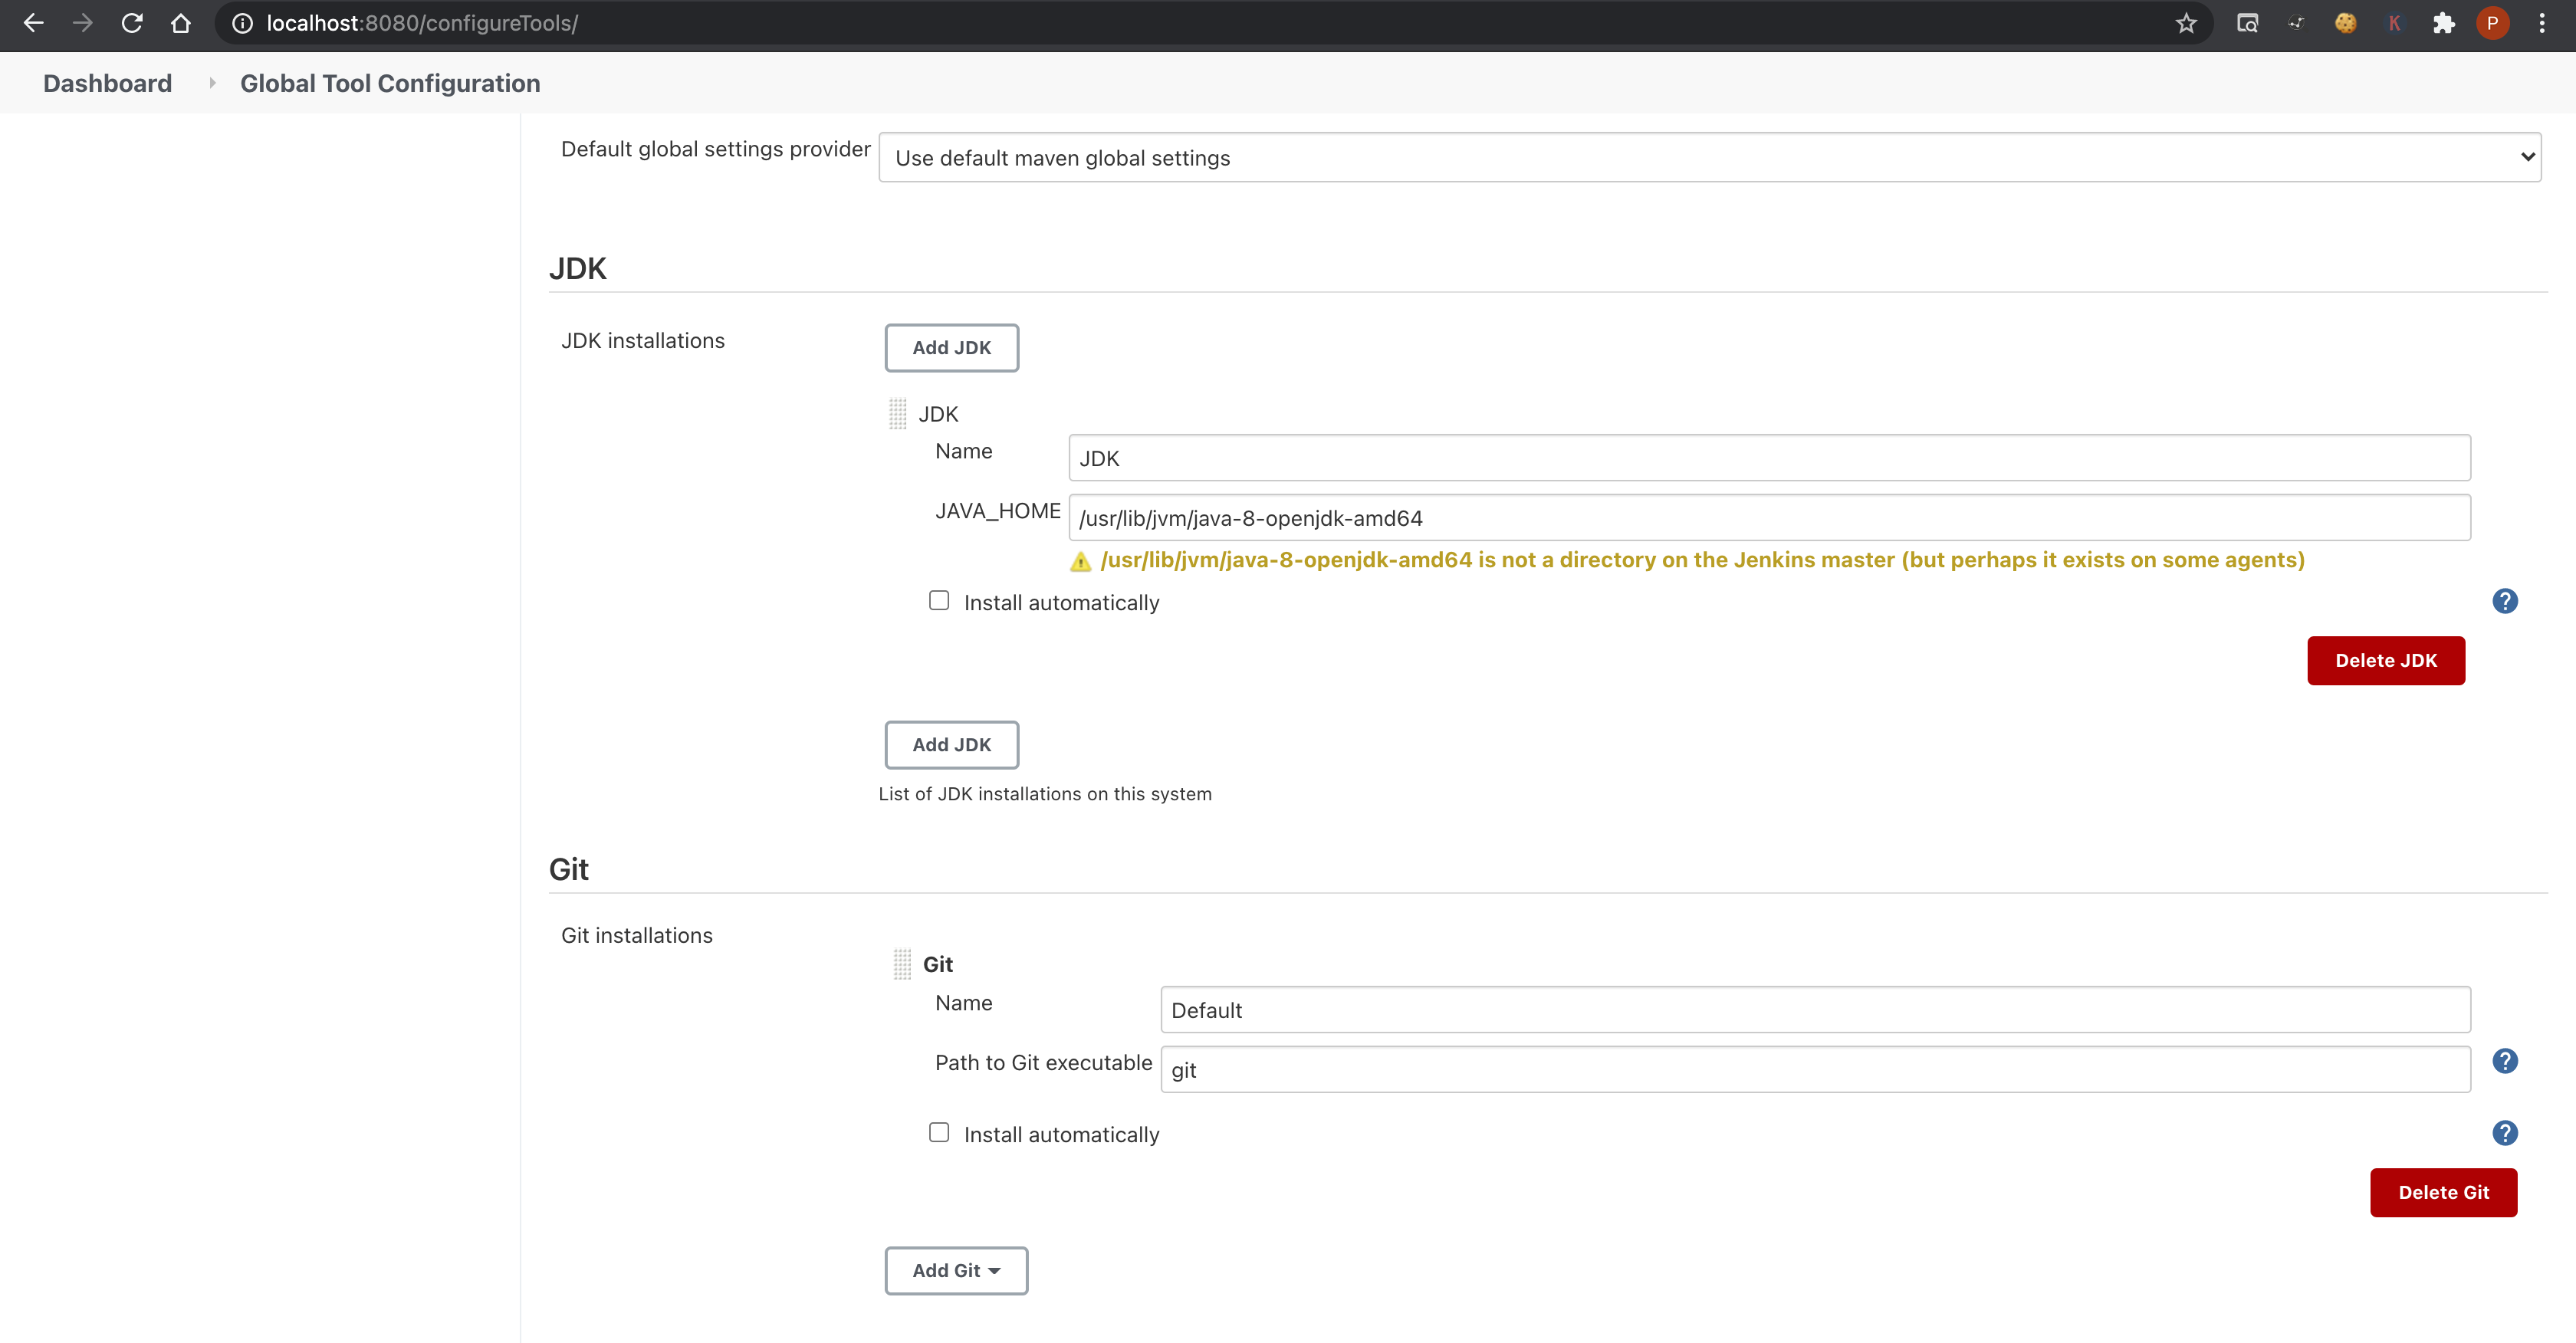
\includegraphics[width=10cm]{iz-JKD-Git.png}
    \caption{JDK-Git}
    \label{fig:JDK-Git}
\end{figure}
\begin{figure}[htbp]
    \centering
    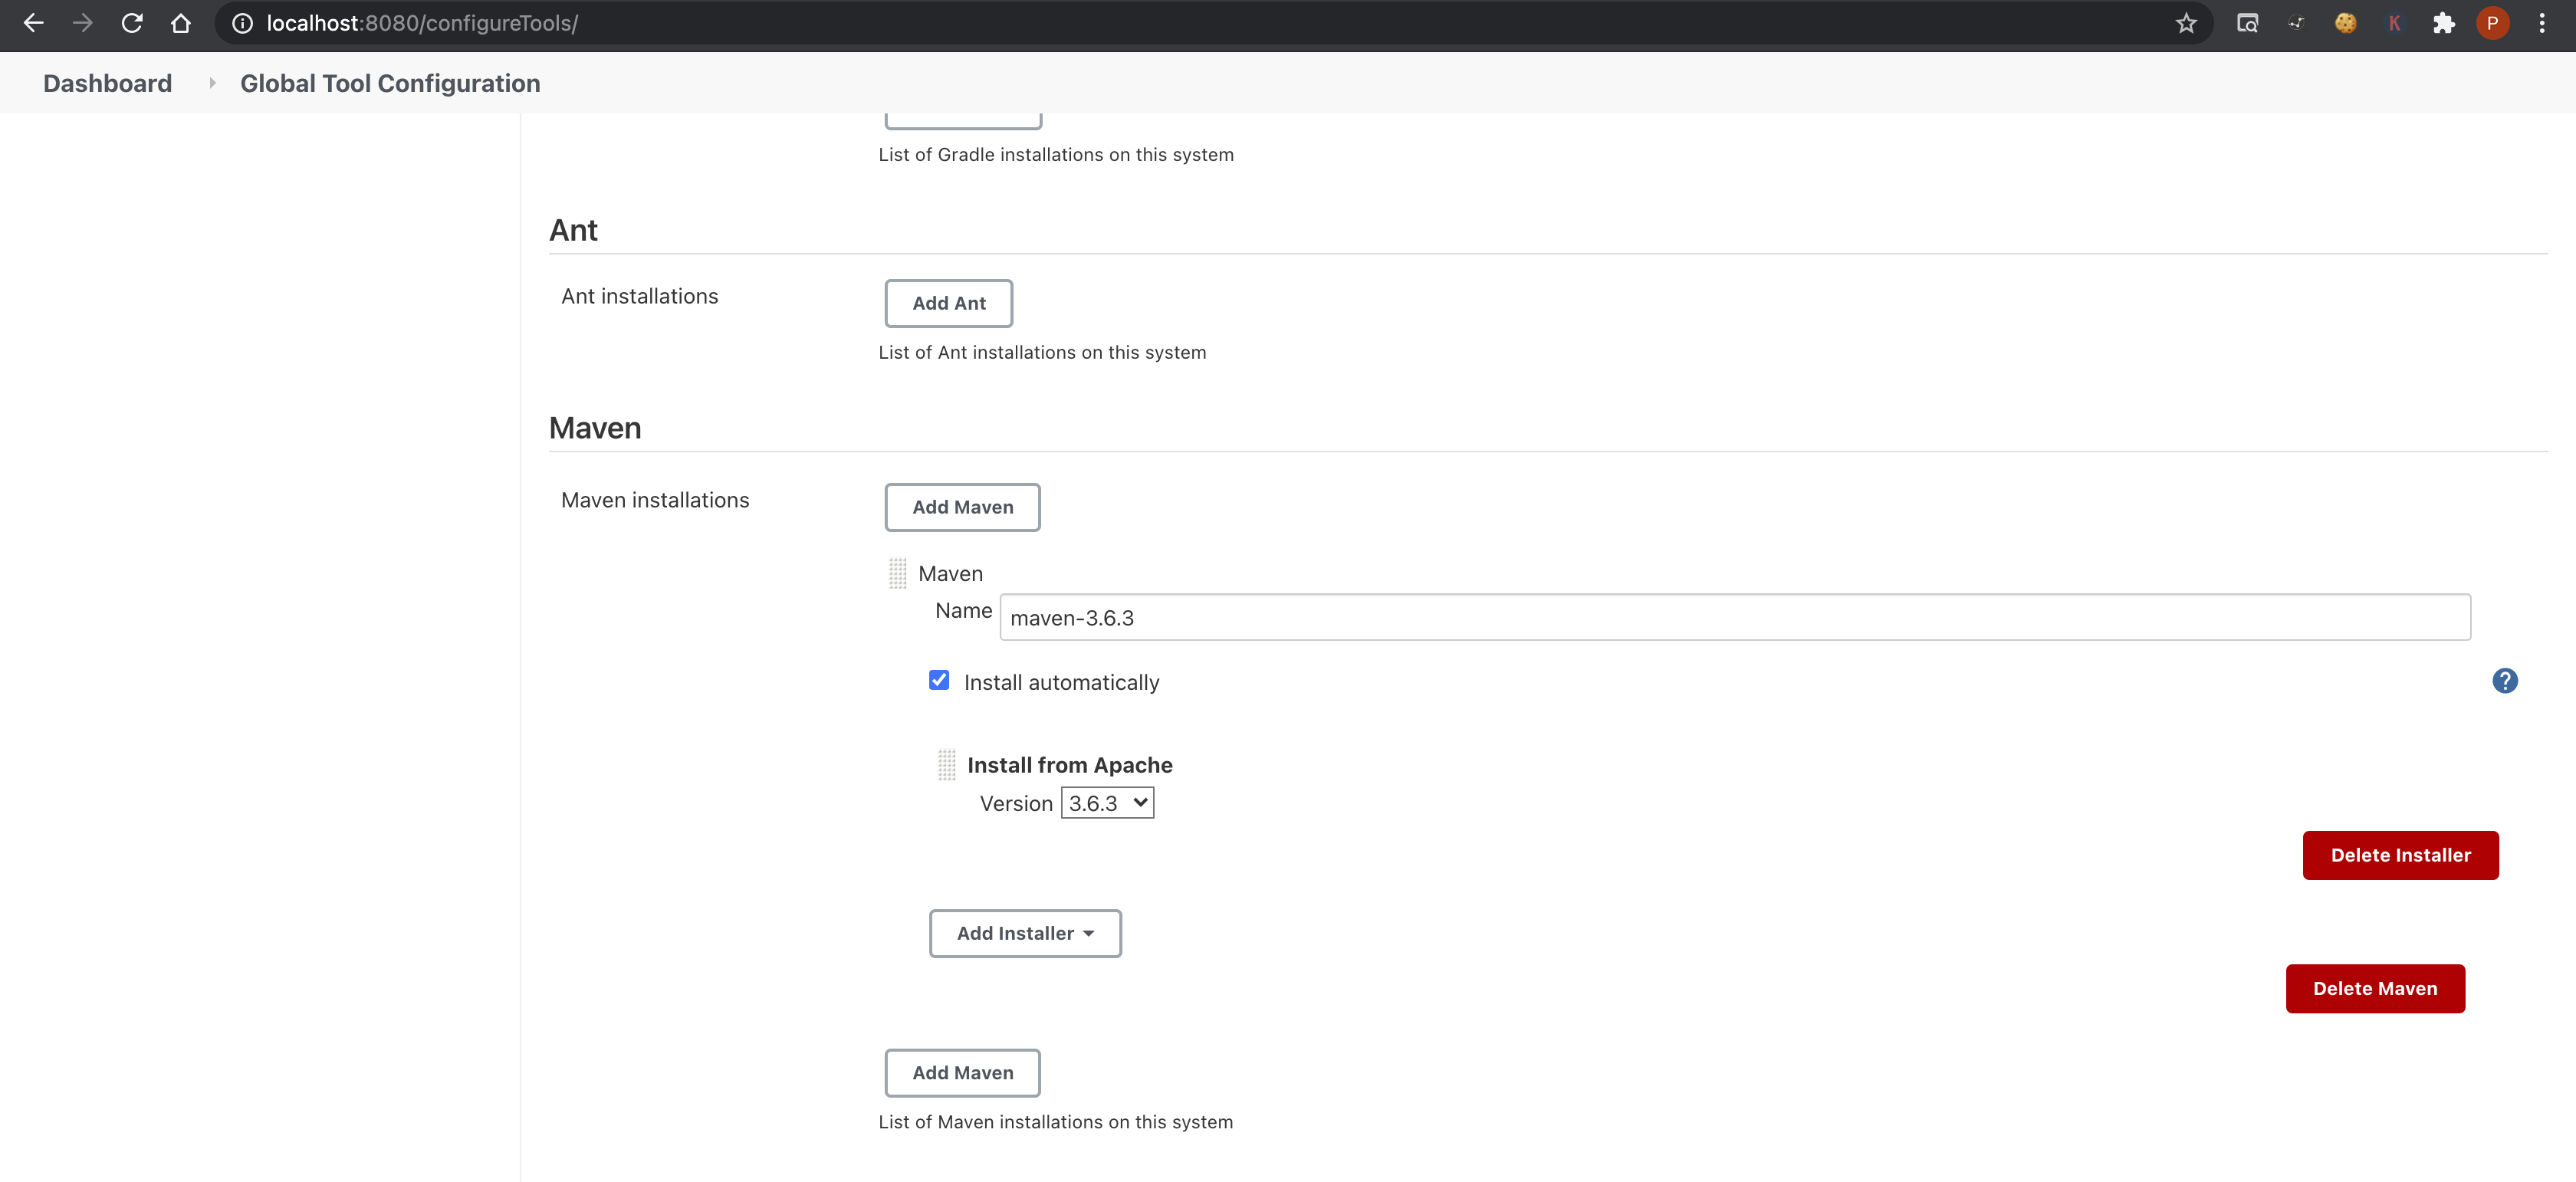
\includegraphics[width=10cm]{iz-maven.png}
    \caption{maven}
    \label{fig:maven}
\end{figure}
\begin{figure}[htbp]
    \centering
    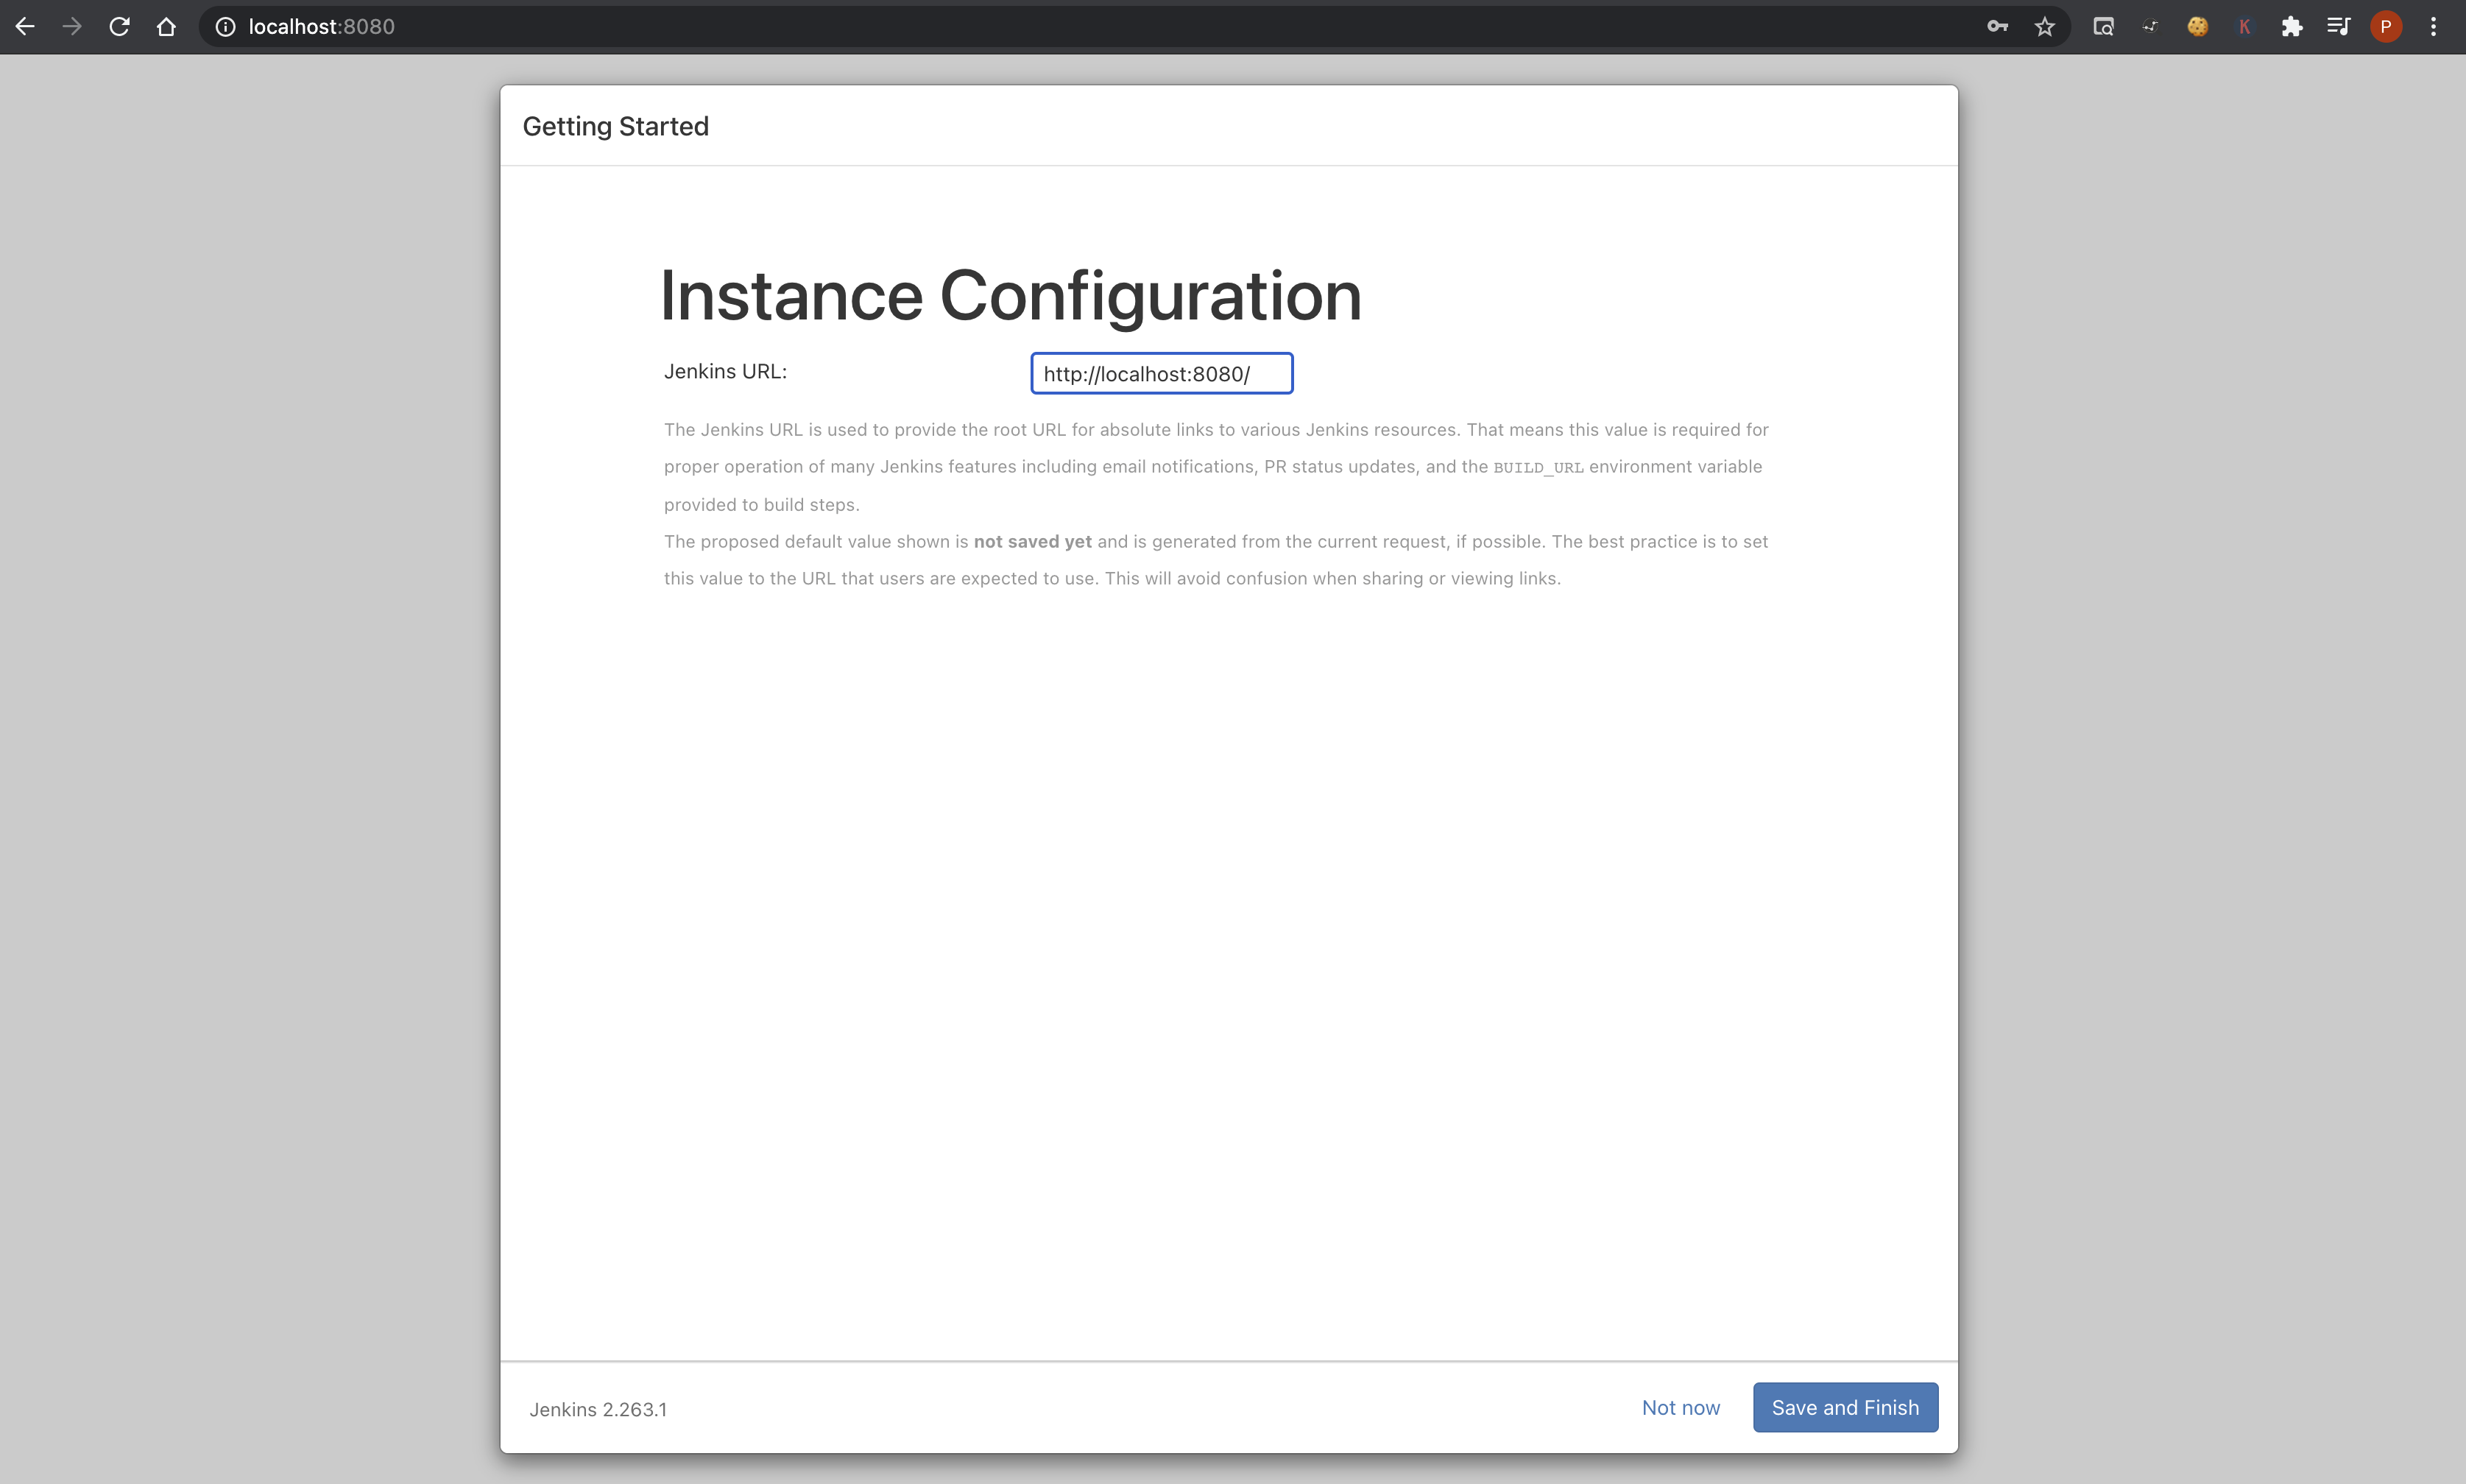
\includegraphics[width=10cm]{iz-Jenkins-port.png}
    \caption{Jenkins port}
    \label{fig:Jenkins-port}
\end{figure}
\begin{figure}[htbp]
    \centering
    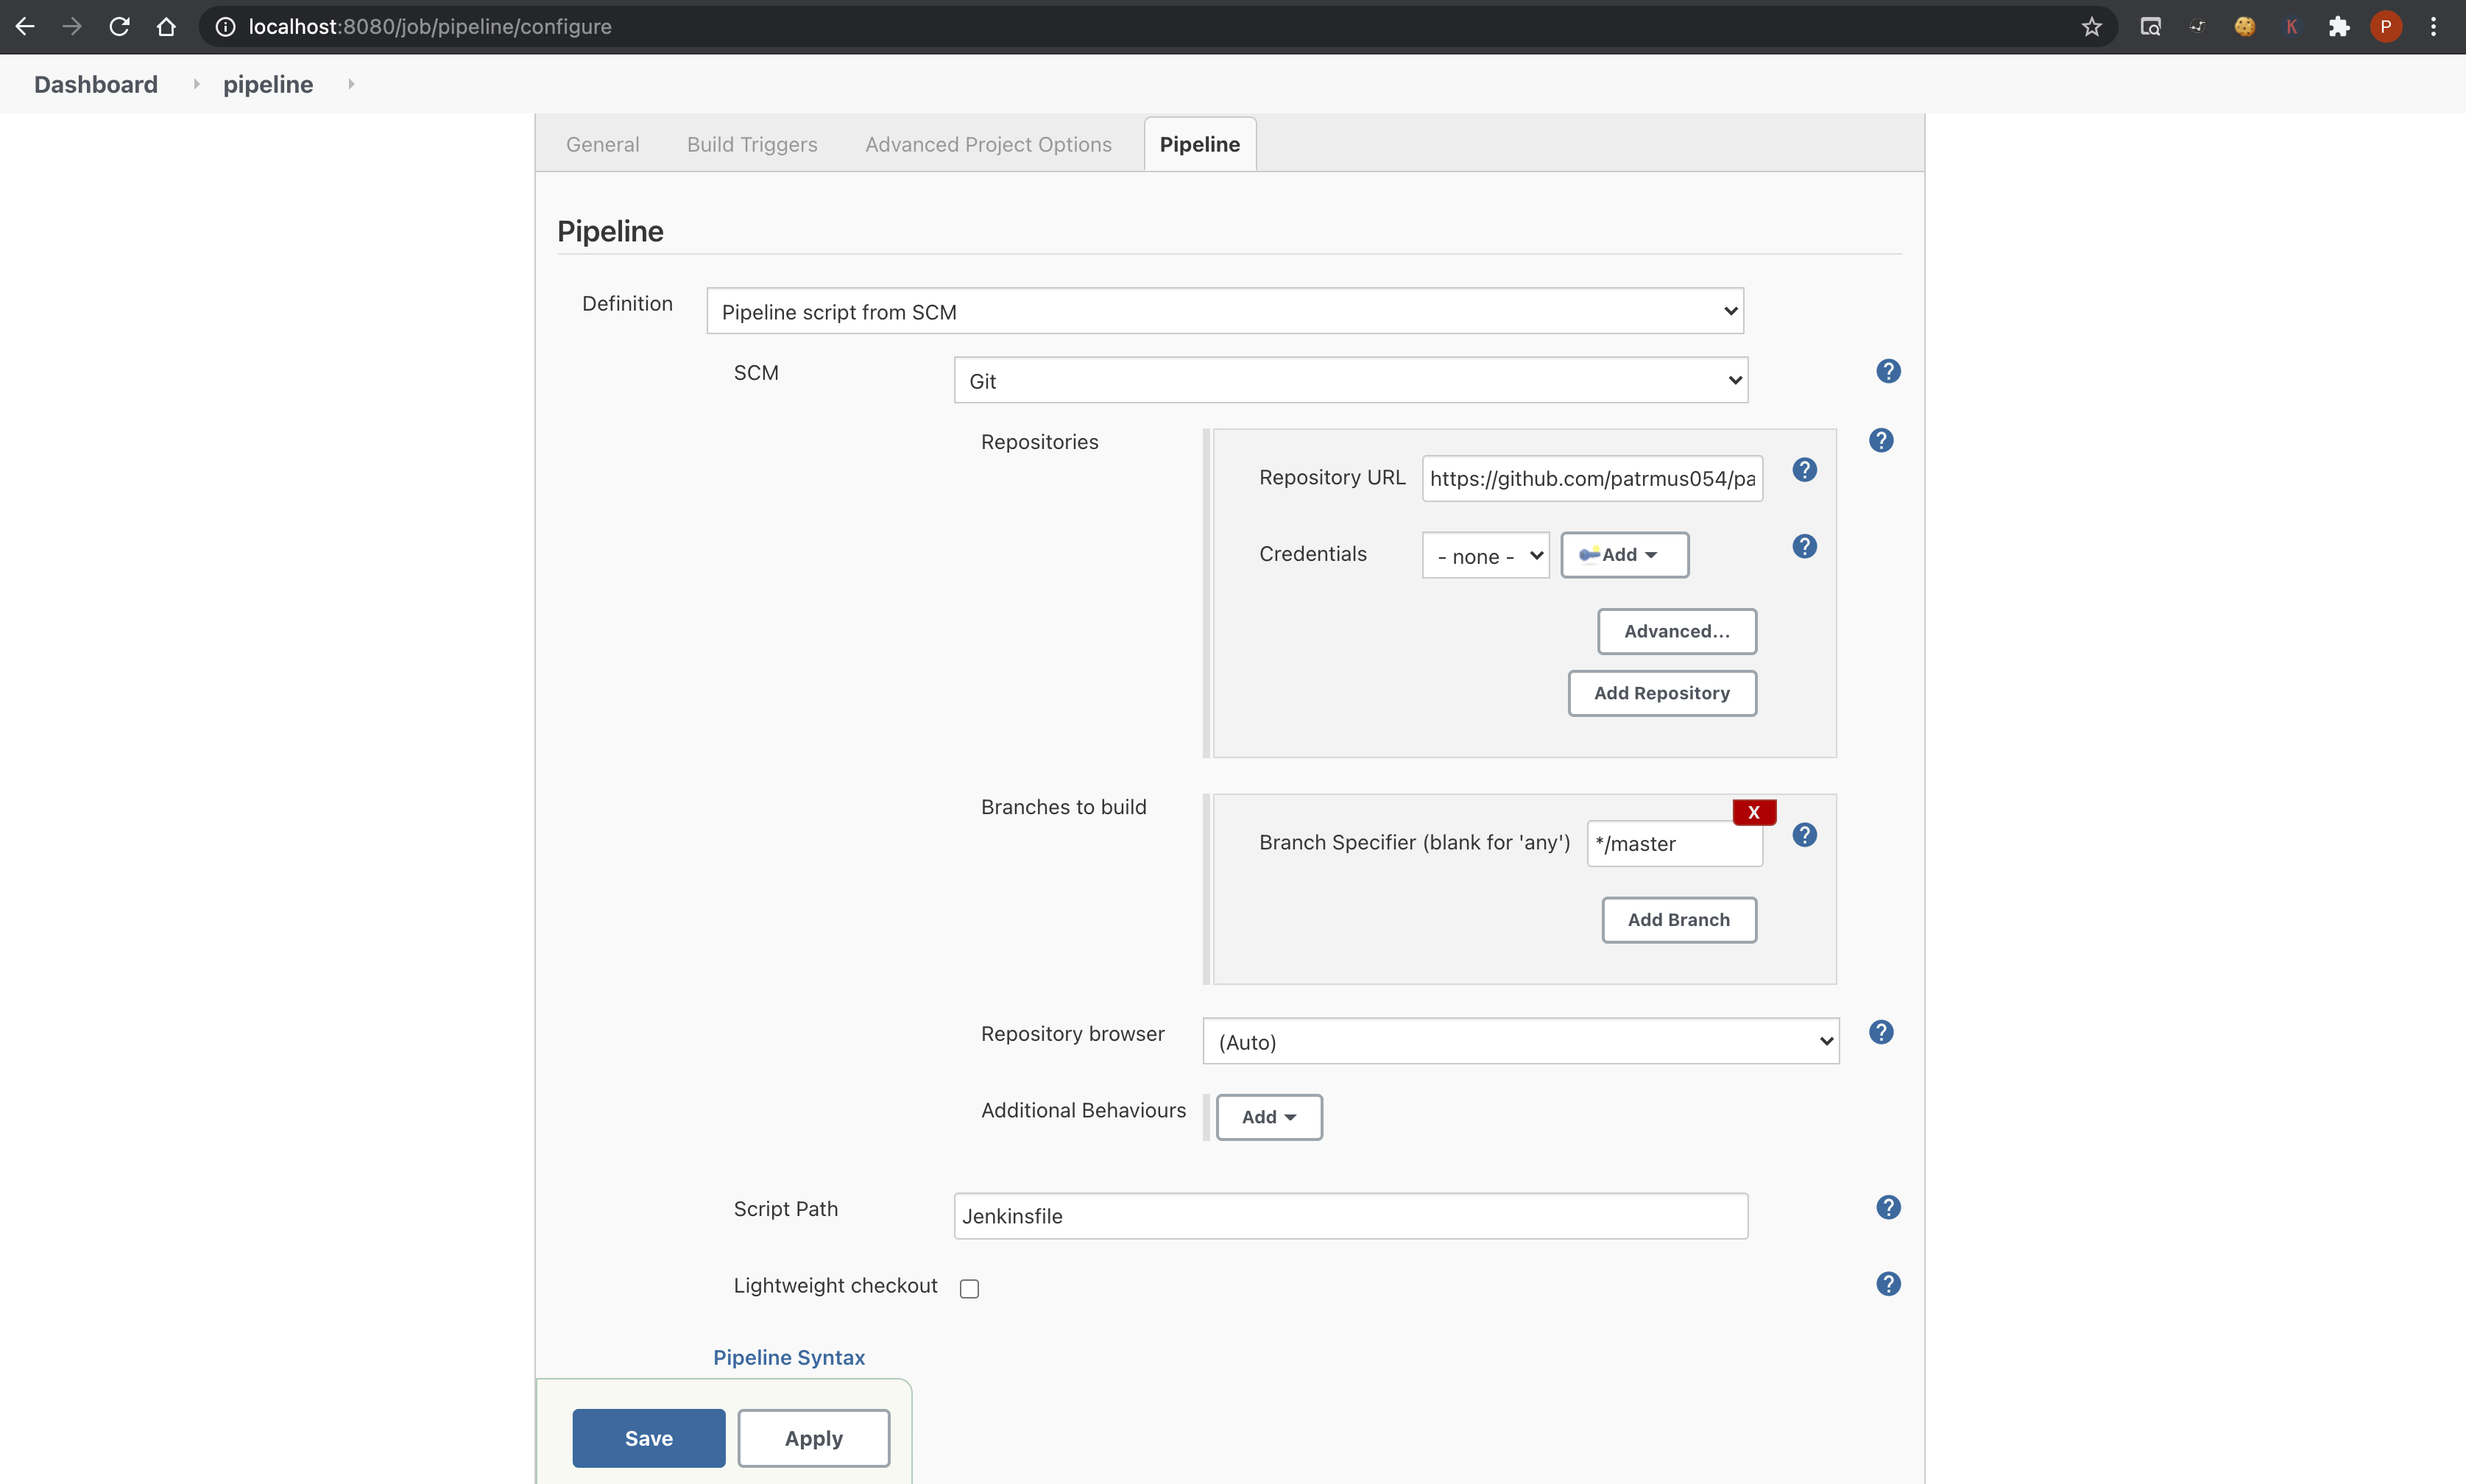
\includegraphics[width=10cm]{iz-pipline.png}
    \caption{pipline}
    \label{fig:pipeline}
\end{figure}


\subsection{Jenkinsfile} 
Jankinsfile jest plikiem w, którym definujemy wszytkie kroki, które mają zostać podjęte w ramach Jenkins pipeline. Mamy możliwość wónierz które zadania na jakich slaveach mają zostać wykonane oraz inne metody konfiguracji pipline'u

W naszym projekcie plik ten składa się z czterech następujączych kroków 

\begin{lstlisting}
    node {  
        
	    def mvnHome = tool 'maven-3.6.3'
	    def dockerImage
	    def dockerImageTag = "pracainzynierka${env.BUILD_NUMBER}"
		def DOCKER_FILES_DIR = "./initial"
		def dockerfile = "Dockerfile"
	    
	    stage('Clone Repo') { // for display purposes
	      git 'https://github.com/patrmus054/papryk-inzynier.git'           
	      mvnHome = tool 'maven-3.6.3'
	    }    
	  
	    stage('Build Project') {
	      sh "'${mvnHome}/bin/mvn' clean install -f ./initial/pom.xml"
	    }
			
	    stage('Build Docker Image') {
	      dockerImage = docker.build("pracainzynierka:${env.BUILD_NUMBER}", "-f ${DOCKER_FILES_DIR}/${dockerfile} ${DOCKER_FILES_DIR}")
	    }
	   
	    stage('Deploy Docker Image'){
	      echo "Docker Image Tag Name: ${dockerImageTag}"
		  sh "docker run pracainzynierka:${env.BUILD_NUMBER} -p 2222:2222 "
	    }
}
\end{lstlisting}

Na początku pliku definujemy zmienne lokalne, potem w kolejnych krokach zasadniczo wszystkie kroki, które musieliśmy wcześniej wpisywać "ręcznie" : pobranie projektu z repozytorium, budowanie aplikacji, budowanie obrazu Dockera i uruchamianie aplikacji. 

\subsection{Podsumowanie projektu}

W dzisiejszym środowisku IT mamy mnogość narzędzi które pozwalają w stosunkowo prosty sposów automatyzować procesy związane z inżyninerią oprogramowania i nie tylko. Jenkins jest od w branży od pewnego czasu i dzięki rozbudowanemu ekosystemowi mamy możliwość automatyzować rzeczy, które wcześniej zajmowały dużo czasu. W projekcie wykorzystaliśmy możliwości narzędzia do stworzenia dwóch działających kontynerów. Rozwiązanie ma jedynie charakter prezentacyjny i nie powinno stanowić inspiracji do produkcji przemysłowej. 

\section{Platformy SaaS z wbudowanym CI/CD}
\subsection{Z czego wynika popularność platform SaaS?}
Platformy takie jak GitHub, CircleCI czy też BitBucket zasłynęły z tego, że oferowały możliwość hostowania naszego repozytorium Git'owego w chmurze. Z biegiem czasu zaczęły one oferować dodatkowe usługi. Serwisy te to już nie tylko miejsce, które umożliwia hostowanie naszego repozytorium kodu - pozwalają one na takie rzeczy jak:
\begin{itemize}
    \item Odpalanie procesów automatyzujących (GitHub, GitLab, BitBucket) - dzięki możliwości tworzenia własnych procesów automatyzujących mamy możliwość zaimplementować własny proces ciągłej integracji, ciągłego dowożenia czy też ciągłego dostarczania,
    \item Odpalanie manualne predefiniowanych procesów (GitLab) - jest to dość prosta funkcjonalność, która daje sporo możliwości. GitLab dostarcza interfejs, w którym możemy uruchomić dowolny pipeline (z ang. \textit{potok}) manualnie - dodatkowo możemy podać argumenty w postaci pól tekstowych. Przykładem, gdzie ta funkcja GitLab'a byłaby użyteczna, jest aplikacja webowa, która zabiera dużo zasobów. Użycie procesu ciągłego dostarczania, by uruchamiać wersję staging'ową oznaczałoby, że aplikacja ta zbędnie używałaby zasoby na serwerze. Dzięki funkcji odpalania manualnego pipeline'ów moglibyśmy uruchamiać aplikację tylko wtedy, kiedy chcielibyśmy przetestować jak działa,
    \item Integracja z Kubernetes'em (GitLab) - GitLab upraszcza proces release'u naszego oprogramowania dzięki integracji z Kubernetes'em. Możemy podpiąć istniejący już klaster albo stworzyć nowy. GitLab może stworzyć taki klaster za nas pod warunkiem, że będzie on działał na chmurze AWS albo Google Cloud,
    \item Publikacje strony statycznej (GitHub) - GitHub umożliwia publikacje danego folderu z plikami statycznymi strony internetowej, który jest częścią repozytorium. Dzięki temu możemy uprościć proces publikacji naszej strony internetowej,
    \item Hosting obrazów Docker'owych oraz paczek/bibliotek (GitHub, GitLab, BitBucket) - dzięki hostingowi obrazów Docker'owych możemy uprościć proces późniejszego odpalenia naszego kodu na serwerze. Dodatkowo możemy hostować na tych platformach paczki popularnych języków. Wspierane są między innymi: NPM (nodeJS), Maven (Java), NuGet (.NET), RubyGems (Ruby),
    \item Śledzenia zadań (GitHub, GitLab, BitBucket) - każda ze znaczących platform ma wbudowane w sobie oprogramowanie do śledzenia zadań. Dzięki temu możemy stworzyć prostą metodykę Agile'ową używając tego, co zapewnia nam dana platforma. Z reguły oprogramowanie to jest mocno ograniczone i nadaje się do prostszych projektów. Zespoły, które mają większe wymagania, muszą szukać oddzielnego oprogramowania,
    \item Audyt bezpieczeństwa bibliotek (GitHub, GitLab) - dzięki tej funkcjonalności możemy się dowiedzieć, czy nasze zależności trzecie nie posiadają luk bezpieczeństwa. GitHub lub GitLab w przypadku wykrycia takiego problemu wysyła maila z powiadomieniem oraz tworzy automatyczną poprawkę,
    \item Sponsoring (GitHub) - GitHub posiada wbudowaną opcję która włącza sponsoring naszego projektu. Dzięki temu na stronie głównej repozytorium pojawia się ikonka serca, która pozwala wesprzeć dany projekt pieniężnie. Jest to ciekawa opcja dla projektów open source.
\end{itemize}
Powyższe funkcjonalności czynią te platformy narzędziami all-in-one (z ang. wszystko w jednym). Dzięki temu, że są one oferowane jako serwisy SaaS, czas który musimy poświęcić na utrzymanie i instalację ogranicza się do zera.
\par
Należy pamiętać, że użycie platform SaaS ma dwie strony medalu. Jeżeli nasz projekt jest publiczny, większość z powyższych usług jest oferowana za darmo. Natomiast jeżeli nasz projekt posiada kod, który jest prywatny, będziemy musieli uiścić odpowiednią opłatę. Zazwyczaj opłata ta jest uzależniona od liczby usług, z których będziemy korzystać oraz od minut automatycznych procesów, które zużyjemy. Platformę na której będziemy działać należy dobrać do indywidualnych potrzeb danego projektu - każda z nich oferuje swoiste ekskluzywne funkcjonalności. Jeżeli naszym celem jest stworzenie statycznej strony, najlepszym wyborem wydaje się GitHub, który oferuje darmowy hosting. Z drugiej strony jeśli zależy nam na uruchamianiu procesów automatyzujących manualnie to powinniśmy spojrzeć w stronę GitLab'a. GitHub jest świetnym rozwiązaniem dla projektów open source, ponieważ większość dodatkowych usług dla takich projektów jest oferowana za darmo. Wynika to z polityki, która została obrana przez właściciela - Microsoft.
\subsection{Strona statyczna - przykład użycia GitHub Actions i GitHub Pages}
Załóżmy, że chcielibyśmy stworzyć stronę internetową, która pozwoliłaby nam przedstawić kim jesteśmy. Mamy następujące wymagania:
\begin{itemize}
    \item Strona ma być statyczna. Dzięki temu będziemy mogli wykorzystać hosting plików, który często jest oferowany jako darmowa opcja,
    \item Strona powinna mieć co najmniej dwie podstrony, które zawierają wspólne sekcje: nagłówek oraz stopkę,
    \item Strona ma być dostępna w sieci za pomocą promowanego przez przeglądarki protokołu HTTPS.
\end{itemize}
By ułatwić sobie powyższe zadanie, użyjemy framework'a Gatsby.js. Jest to generator stron statycznych, który upraszcza tworzenie takowych stron. Framework używa popularną bibliotekę React, która pozwala korzystać z składni JSX (składnia mocno przypomina format HTML). Główną cechą Gatsby'iego jest to, że zapewnia integracje z popularnymi systemami takimi jak Wordpress \cite{GatsbyJSWordpress}. Dzięki temu nie jesteśmy zmuszeni utrzymywać dedykowanego serwera PHP - Gatsby wygeneruje wszystkie możliwe podstrony podczas procesu budowania strony. Jest to szczególnie ciekawe rozwiązanie dla serwisów, które generują duży ruch. Znacznie łatwiej serwować pliki statyczne niż za każdym razem budować stronę, obciążając dodatkowo bazę danych.
\par
Gatsby.js w postaci programu działającego w wierszu poleceń pozwala w prosty sposób pobrać startowy szablon z minimalnym zbiorem potrzebnych rzeczy. Użyjmy tego szablonu jako punktu wejściowego:
\begin{lstlisting}[caption={Pobierania szablonu startowego}]
    gatsby new static-website-with-ci-cd https://github.com/gatsbyjs/gatsby-starter-default
\end{lstlisting}
Domyślny szablon posiada w dużej mierze gotowy layout z nagłówkiem oraz stopką. Jest on zdefiniowany w pliku 'src/components/layout.js'. Po małej przeróbce wygląda on następująco:
\begin{lstlisting}[caption={Layout - komponent zawierający logikę związaną z layoutem strony}]
    const Layout = ({ children }) => {
        const data = useStaticQuery(graphql`
          query SiteTitleQuery {
            site {
              siteMetadata {
                title
              }
            }
          }
        `)
      
        return (
          <>
            <Header siteTitle={data.site.siteMetadata?.title || `Title`} />
            <div
              style={{
                margin: `0 auto`,
                maxWidth: 960,
                padding: `0 1.0875rem 1.45rem`,
              }}
            >
              <main>{children}</main>
              <footer style={{
                marginTop: `2rem`
              }}>
                Stopka
              </footer>
            </div>
          </>
        )
    }
\end{lstlisting}
Dzięki temu, że zawartość sekcji \textit{$<$main$>$} jest konfigurowalna za pomocą argumentu \textit{children}, możemy współdzielić layout między różnymi podstronami.
\par
Pierwszą stroną, którą chcielibyśmy stworzyć, jest strona domowa. Na niej wyświetlimy podstawowe informacje o nas oraz umieścimy link do strony, na której przedstawimy więcej danych o sobie. Kod tej strony jest stosunkowo prosty:
\begin{lstlisting}[caption={index.js - plik zawiera treść strony domowej}]
  import React from "react"
  import { Link } from "gatsby"
  import Layout from "../components/layout"
  import SEO from "../components/seo"
  import MeImgSrc from "../images/ja.jpg"

  const IndexPage = () => (
    <Layout>
      <SEO title="Home" />
      <div>
        <h2>Artur Kasperek - Programista oraz Student Politechniki Slaskiej</h2>
        <img src={MeImgSrc}/>
      </div>
      <div>
        <Link to="/detale">Wiecej o mnie</Link> <br />
      </div>
    </Layout>
  )

  export default IndexPage
\end{lstlisting}
Drugą stroną jest podstrona, która wyświetla więcej szczegółów. Podobnie jak na stronie domowej zawiera link do głównej strony. Zawartość wygląda następująco:
\begin{lstlisting}[caption={detale.js - plik zawiera treść strony z szczegółami}]
  import React from "react"
  import { Link } from "gatsby"

  import Layout from "../components/layout"
  import SEO from "../components/seo"

  const SecondPage = () => (
    <Layout>
      <SEO title="Detale" />
      <h2>Doswiadczenie</h2>
      <ul>
        <li>JavaScript</li>
        <li>HTML</li>
        <li>CSS</li>
        <li>C++</li>
        <li>NodeJS</li>
      </ul>
      <h2>Szkoly</h2>
      <ul>
        <li>Politechnika Slaska</li>
        <li>I Liceum Ogolnoksztalcacego im. Stefana Zeromskiego w Zawierciu</li>
        <li>Gimnazjum nr 1 Zawierciu</li>
      </ul>
      <Link to="/">Powrot do strony domowej</Link>
    </Layout>
  )

  export default SecondPage

\end{lstlisting}
\par
Strona może być teraz opublikowana. Do tego celu służy komenda \textit{gatsby build}. Komenda ta buduje stronę i umieszcza ją w folderze \textit{public}. Chcielibyśmy teraz w jakiś sposób opublikować stronę w sieci. W tym celu możemy skorzystać z usługi GitHub Pages. Wymogiem jest tutaj to, by nasz kod strony internetowej był repozytorium Git'owym trzymanym na GitHub'ie. Po tym, gdy nasz projekt jest już repozytorium Git'owym na GitHub'ie, możemy stworzyć definicję potoku ciągłego dowożenia. Chcielibyśmy, by za każdym razem, gdy nowy kod zostaje wysłany na gałąź \textit{master}, strona się budowała i była publikowana w sieci.
\par
GitHub Actions posiada własną składnię do definicji potoków automatyzujących. Najmniejszą jednostką, którą możemy zdefiniować jest \textit{workflow} (z ang. \textit{przepływ}). W dokumentacji \cite{GithubActionsDoc} możemy dowiedzieć się, że \textit{workflow} to konfigurowalny zautomatyzowany proces składający się z co najmniej jednego zadania oraz pliku YAML, który zawiera jego definicję. Warto podkreślić, że plik ten jest częścią naszego projektu - wynika z tego, że jest on wersjonowany wraz z kodem źródłowym i innymi plikami.
\par
Plik YAML danego \textit{workflow} zawiera informację o swojej nazwie, to kiedy ma się odpalić oraz definicję tego co ma wykonać. W naszym przypadku chcemy, by nasz \textit{workflow} wykonywał się za każdym razem, gdy wrzucamy jakieś zmiany na master'a. Możemy to osiągnąć za pomocą poniższego fragmentu kodu:
\begin{lstlisting}[caption={Nazwa oraz definicja wyzwalacza \textit{workflow} budującęgo stronę}]
  name: Build and Deploy

  on:
    push:
      branches: [ master ]
\end{lstlisting}
\par
Kolejnym krokiem jest zdefiniowanie to, co nasz \textit{workflow} ma robić. W naszym przypadku chcielibyśmy zbudować stronę oraz opublikować ją za pomocą GitHub Pages. W tym celu w ustawieniach projektu włączamy GitHub Pages oraz definiujemy, w jakim folderze oraz na jakiej gałęzi będą dostępne pliki statyczne strony. W naszym przypadku wybieramy gałąź \textit{gh-pages} oraz główny folder.
\begin{figure}[htbp]
  \centering
  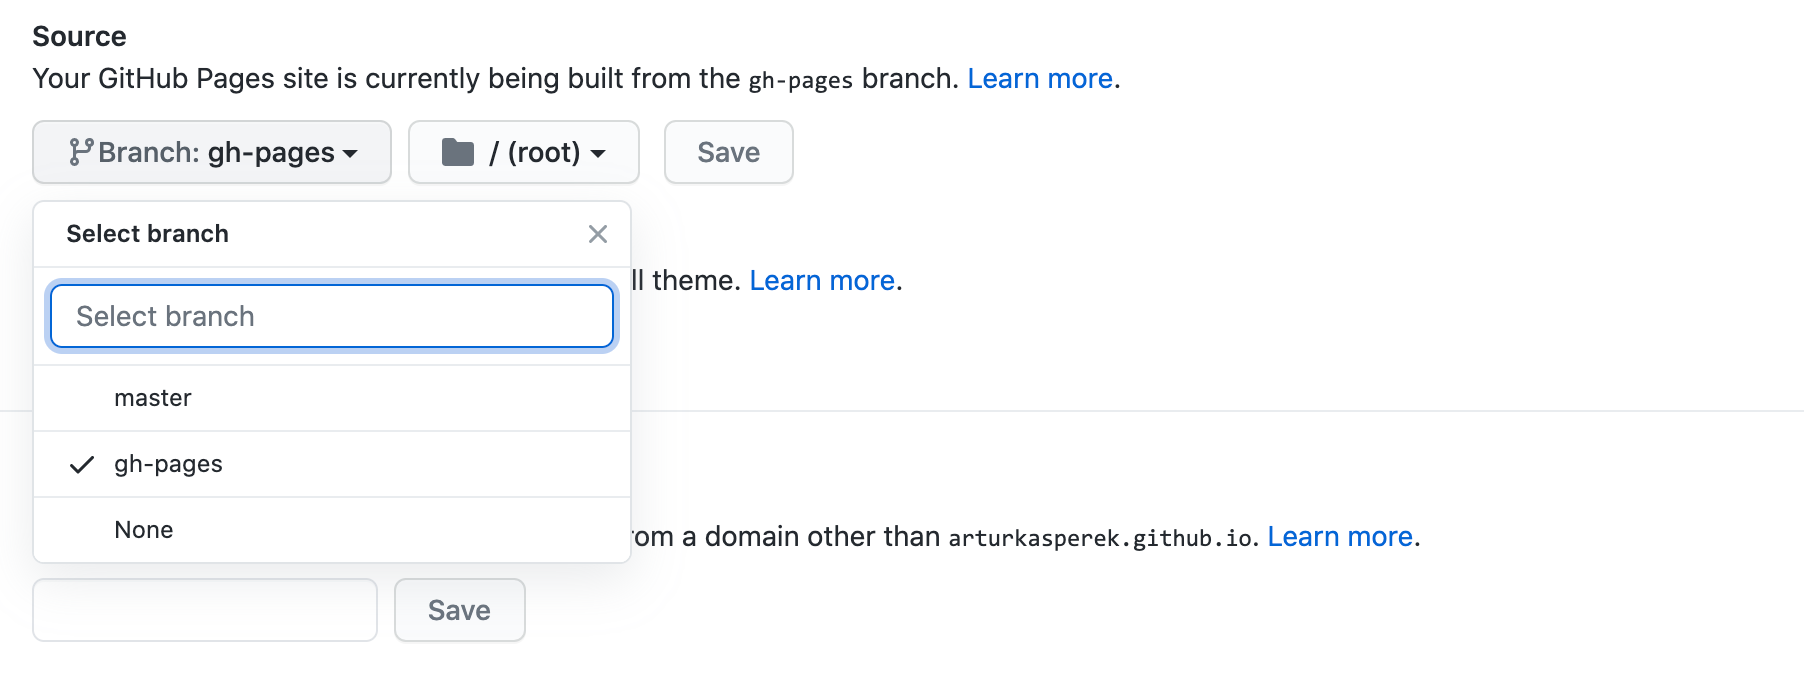
\includegraphics[width=12cm]{gh_pages.png}
  \caption{Ustawienia GitHub Pages}
  \label{fig:gh_pages}
\end{figure}
Dzięki temu będziemy w stanie odseparować gałąź, gdzie trzymamy kod źródłowy strony, od zbudowanej statycznej strony. Jest to także ułatwienie dla potoku automatyzującego. Jeżeli chcielibyśmy zapisywać zbudowaną stronę na gałęzi \textit{master}, oznaczałoby to, że nasz \textit{workflow} wyzwalałby się w nieskończoność przez fakt, iż jest on uzależniony od tego, czy jakieś nowe zmiany zostały wysłane na gałąź \textit{master}.
\par
Definicja tego, co nasz proces ciągłego dowożenia ma robić, wygląda następująco:
\begin{lstlisting}[caption={Definicja zadań \textit{workflow}'a budującego stronę}]
  jobs:
    build-and-deploy:
      runs-on: ubuntu-latest
      steps:
      - uses: actions/checkout@v2
      - name: Use Node.js 14.x
        uses: actions/setup-node@v1
        with:
          node-version: 14.x
      - name: Install Dependencies
        run: |
          yarn install
      - name: Build website
        run: |
          yarn build
      - name: Deploy
        uses: JamesIves/github-pages-deploy-action@3.6.2
        with:
          GITHUB_TOKEN: ${{ secrets.GITHUB_TOKEN }}
          BRANCH: gh-pages
          FOLDER: public
          CLEAN: true
\end{lstlisting}
\par
Jedną z rzeczy, które wyróżniają GitHub Actions nad innymi systemami ciągłej integracji/ciągłego dowożenia, jest możliwość definiowania tytułowych akcji. Akcje to nic innego jak sprytnie zapakowane programy lub też skrypty bash'owe, które pod spodem wykonują jakąś skomplikowaną rzecz. W zależności od argumentów środowiskowych możemy daną akcję dostosować do naszych potrzeb. Z faktu, że każdy może publikować własne akcje, nie jesteśmy ograniczeni do korzystania tylko z akcji dostarczonych przez twórców GitHub Actions. Dzięki takiemu podejściu mamy dostęp do bogatej bazy gotowych modułów.
\par
Wyjaśnijmy teraz, co dane linijki robią. W linii 3 definiujemy to, jaki system chcemy użyć jako bazowy. W naszym przypadku używamy Ubuntu, ponieważ jest najbardziej „lekkim” z wszystkich możliwych systemów. Od linijki 4 do końca mamy definicję kroków, co dany \textit{job} (z ang. \textit{zadanie}) ma wykonać. Pierwszymi krokami jest przełączenie się do danego branch'a oraz użycie akcji, która zainstaluje nam środowisko nodeJS w wersji 14. Od linii 10 do 15 zdefiniowane są dwa kroki, których celem jest zainstalowanie zależności naszego projektu oraz jego zbudowanie. W tym celu używamy menadżera paczek \textit{yarn}, który został zainstalowany dodatkowo podczas instalacji nodeJS. Kroki te pokazują, że nie jesteśmy uzależnieni tylko od użycia gotowych akcji. Za pomocą słowa kluczowego \textit{run} możemy zdefiniować dowolną komendę bash'ową, która ma być wykonana w danym momencie. Warto podkreślić fakt, że zmienne środowiskowe, które były zdefiniowane w danym kroku, nie są dostępne dla kolejnych kroków. GitHub Actions odpala każdy krok w osobnej sesji bash'owej. Na ten moment nasza strona powinna być wybudowana i zapisana w folderze \textit{public}.
\par
Ostanim krokiem jest publikacja strony na gałęzi \textit{gh-pages}. W tym celu używamy gotowej akcji o nazwie \textit{JamesIves/github-pages-deploy-action} w wersji 3.6.2. Jest to przykład akcji, która została dostarczona przez trzeciego autora i jest udostępniona szerokiej publiczności. Akcja ta „pod spodem” za pomocą git'a wysyła dany folder na wyspecjalizowaną za pomocą parametru \textit{BRANCH} gałąź. Dodatkowo musimy podać w parametrach akcji token dostępu do GitHuba. Robimy to za pomocą parametru \textit{GITHUB\_TOKEN}. Token ten jest automatycznie generowany przez GitHub'a podczas odpalania danego \textit{workflow}'a i daje możliwość zapisywania zmian do repozytorium, gdzie \textit{workflow} jest odpalane. Tym sposobem akcja dostaje niezbędne prawa do wysłania folderu z wybudowaną stroną na gałąź \textit{gh-pages}, która jest częścią tego samego repozytorium. Dzięki temu, że wykorzystaliśmy gotową akcję do publikacji naszej strony, ograniczyliśmy długość kodu oraz zredukowaliśmy czas, który musielibyśmy poświęcić na stworzenie skryptu, który wysyła folder \textit{public} na odpowiednią gałąź.
\par
Teraz, gdy nasze repozytorium posiada plik konfiguracyjny GitHub Actions, w zakładce \textit{Action} na GitHub'ie powinniśmy zauważyć zakolejkowane zadanie budowania strony.
\begin{figure}[htbp]
  \centering
  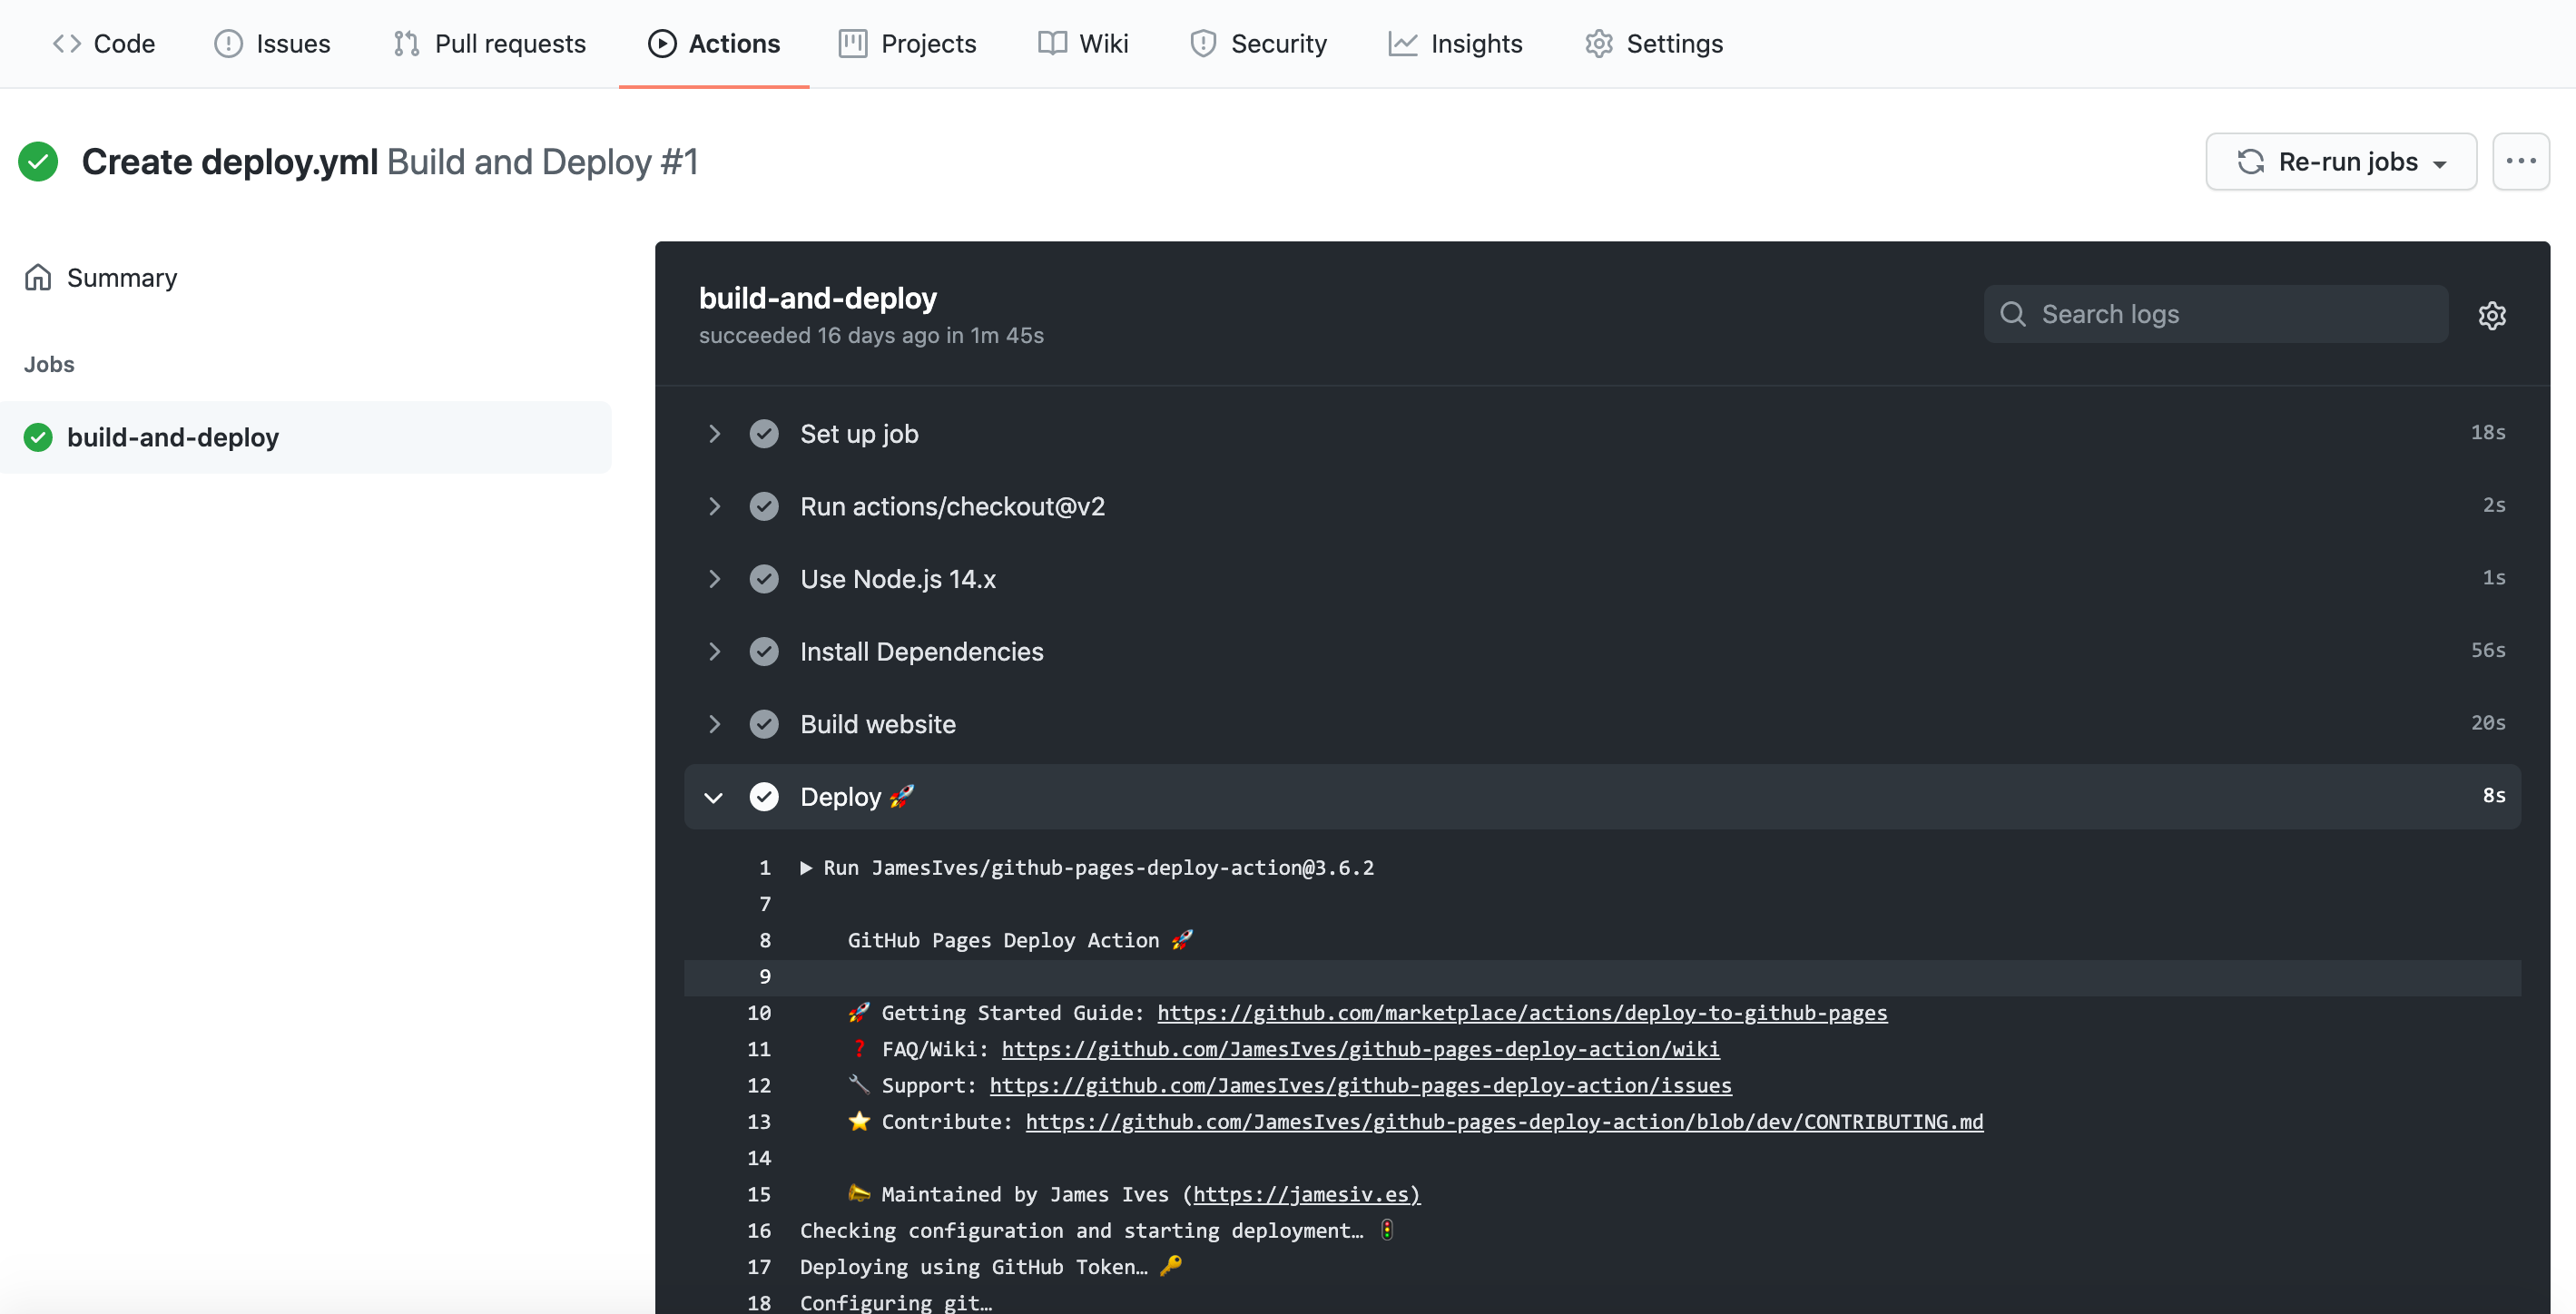
\includegraphics[width=12cm]{gh-actions-log.png}
  \caption{Widok na którym możemy zobaczyć szczegóły danego zadania}
  \label{fig:gh_actions_log}
\end{figure}
Sumarycznie pierwsze budowanie strony zajęło 1min 45sec. Najwięcej czasu zabrało zainstalowanie zależności - aż 56 sekund. Na szczęście GitHub zapewnił akcję, która pozwala cache'ować zależności. Warunkiem koniecznym do działania tego mechanizmu jest posiadanie pliku z informacjami o wersjach zależności jakich używamy. Nie powinno być to problemem, ponieważ większość współczesnych menadżerów zależności generuje taki plik. Implementując cache'owanie, proces automatyzujący będzie tylko instalował zależności, jeżeli jakaś ich wersja się zmieni - w reszcie przypadków proces używa plików z cache'a.
\par
Po tym, gdy pliki z stroną „wylądowały” na gałęzi \textit{gh-pages}, GitHub powinien zakolejkować proces publikacji strony. Jest to rzecz, nad którą nie mamy kontroli.
\begin{figure}[htbp]
  \centering
  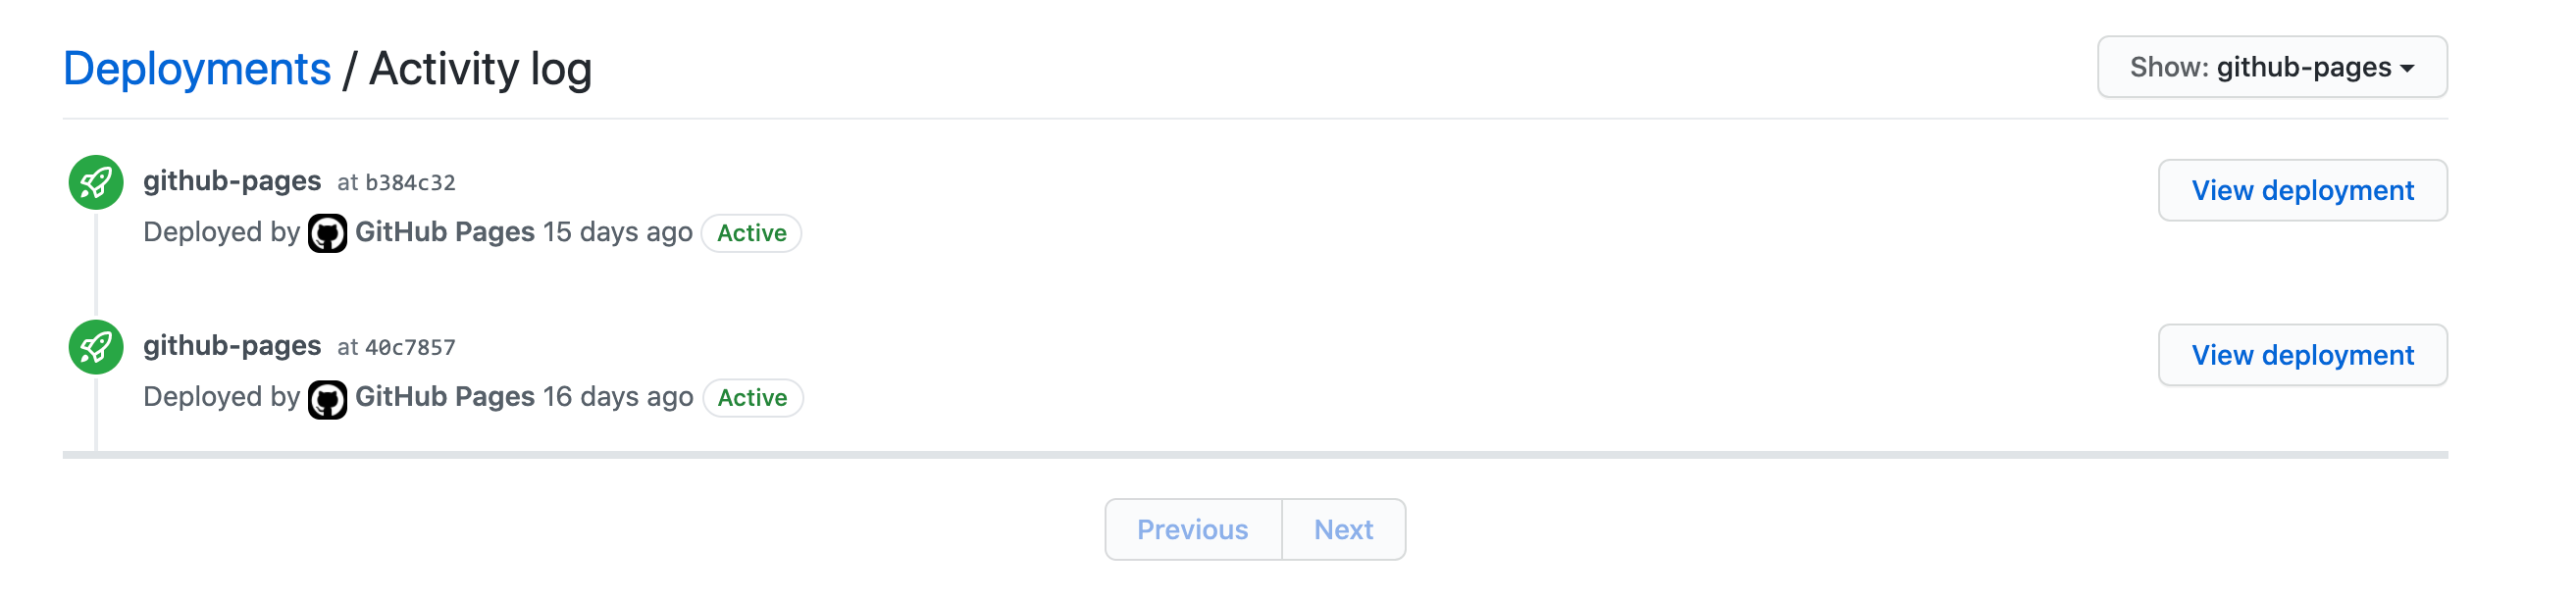
\includegraphics[width=12cm]{gh_pages_deploy.png}
  \caption{Widok z publikacjami strony}
  \label{fig:gh_pages_deploy}
\end{figure}
\par
GitHub wewnętrznie bierze pliki strony z gałęzi, którą ustawiliśmy, i publikuje to na swoich serwerach. Finalnie omawiana strona jest dostępna pod adresem \textit{https://arturkasperek.github.io/static-website-with-ci-cd/}. GitHub pages samo w sobie nie ogranicza nas do używania domeny \textit{github.io}. Jeżeli posiadamy własną domenę, możemy odpowiednio tak przekierować ruch do GitHub'a, że finalny użytkownik nie będzie wiedział, gdzie strona jest hostowana.
\par
Dzięki zapewnieniu modułowości, GitHub Actions może pochwalić się dużą biblioteką akcji stworzoną przez społeczeństwo. Oto lista ciekawych akcji:
\begin{itemize}
  \item jakejarvis/s3-sync-action - jest to akcja, która pozwala synchronizować dany folder repozytorium z folderem na usłudze hostingowej AWS S3. Może być użyteczna, jeżeli chcielibyśmy danej grupie deweloperów dać możliwość wysyłania plików na S3, bez konieczności dawania dostępu do panelu administratora AWS,
  \item repo-sync/github-sync - akcja ta potrafi synchronizować dane repozytorium z innym repozytorium dostępnym w sieci. Jest ona szczególnie użyteczna, gdy pracujemy nad fork'iem (fork to kopia projektu która rozwija się niezależnie względem oryginału) jakiegoś projektu i chcemy utrzymać zgodność z oryginałem. GitHub Actions pozwala na odpalanie danego procesu automatyzującego automatycznie na podstawie planera. Dzięki temu możemy wykorzystać tą akcję, by co jakiś czas synchronizowała nasze repozytorium z macierzystym projektem,
  \item release-drafter/release-drafter - akcja jest szczególnie użyteczna, jeżeli nasz projekt chce korzystać z dobrych praktyk, dotyczących publikacji oprogramowania. Akcja ta oblicza, jakie zmiany w kodzie nastąpiły od ostatniej publikacji i tworzy wstępną publikację na GitHub'ie z opisem zmian, które dokonaliśmy. Akcja ta jest oparta na commit'ach, dlatego warto by one były dobrze opisane. Jeżeli użyjemy odpowiednich prefixów jak \textit{feature} oraz \textit{bug}, akcja będzie w stanie lepiej sformatować opis publikacji,
  \item zaproxy/action-baseline - jest to akcja, która jest oparta o użycie narzędzia ZAP - to program, który analizuje nasz kod pod względem różnorakich luk bezpieczeństwa. Finalnie jeżeli akcja w wyniku swojego działania znajdzie jakieś podatności to tworzy automatycznie \textit{issue} (system na GitHub'ie, który pozwala śledzić błędy). Jest to ciekawa opcja, jeżeli chcemy jak najbardziej zabezpieczyć się przed ewentualnymi atakami hackerów.
\end{itemize}
Wszystkie powyższe rzeczy moglibyśmy wykonać, używając akcji, która odpala skrypt bash'owy. Takie podejście jednak miałoby sporo wad - bylibyśmy zmuszeni spędzić sporo czasu, by wszystko zgrać tak jak chcemy. Dodatkowo prawdopodobnie nie pokrylibyśmy różnych przypadków brzegowych. Dzięki gotowym akcjom czas konfiguracji środowiska do automatyzacji skraca się do minimum, a my możemy się skupić na rozwiązywaniu innych problemów.



% tutaj mógłbym rozwinąć rozdział 3 i powiedzieć, że coraz mniej używa się Jenkinsa i obecnie popularne są platformy jak Github Actions, CircleCI czy gitlabCI, które są trigerrowane przez commity, pushe czy też tworzenie tagów z pomocą systemu wersji git. Myślę, że mógłbym tutaj zrobić nawiązanie do części praktycznej pracy:
% 4a) continues delivery w React Native na przykładzie GitHub actions
% 4b) continues deploymeny na przykładzie aplikacji backendowej w javaScriptcie
% 4c) continues deployment strony internetowej hostowanej przez GitHub actions za pomocą circleCI
% W każdym z tych podrozdziałów opisałbym jaki jest ogólny problem i dalej opisałbym już konkretne rozwiązanie

\section{Testy a continuous integration}
W celu lepszego zrozumienia istoty automatyzacji testów konieczne jest najpiew zrozumienie testów samych w sobie. Jak zostało to opisane w rozdziale 1.4 - pisanie testów jest integralną częścią pracy każdego programisty. Wiele osób uważało to dawniej za żmudne zadanie, nieprzynoszące wymiernych korzyści, jednakże z biegiem czasu stało się jasne, że w dużych projektach informatycznych są one konieczne, co widać w dzisiejszych czasach w wypowiedziach wielu osób. \cite{UnitOpinions} \cite{UnitResults}

\subsection{Testy jednostkowe}
Testem jednostkowym nazywa się kod, który jest w stanie wywołać inny fragment kodu programu, a następnie sprawdzić czy działanie tamtego kodu jest zgodne z zakładanym przez programistę działaniem. \cite{UnitDefinition}
\par Autor tej definicji zdefiniował też kilka warunków, które powinien spełniać każdy test jednostkowy dobrej jakości: 
\begin{itemize}
    \item jest w pełni zautomatyzowany - nie wymaga żadnej interakcji od użytkownika
    \item odizolowany od reszty kodu, którego nie sprawdza oraz od innych testów - w celu spełnienia tego warunku często będą wykorzystywane tak zwane "mocki" oraz "stuby" 
    \item nie ma dostępu do baz danych lub plików na dysku
    \item jest deterministyczny, nie zawiera losowych danych, przy każdym uruchomieniu kodu zwraca taki sam rezultat
    \item jest szybki - należy pamiętać, że testów będzie w kodzie dużo, a także będą one często uruchamiane
    \item skupia się na pojedynczym logicznym elemencie programu
    \item czytelny
    \item łatwy w zrozumieniu
    \item wiarygodny - wynika to z dwóch powyższych warunków. Po otrzymaniu wyniku testów nie powinniśmy mieć wątpliwości czy jest on poprawny
\end{itemize}
Fragmentem kodu, który podlega testom jest zwykle najmniejsza jego część, która odpowiada za jedno logiczne działanie. Najczęściej będzie to więc pojedyncza metoda klasy lub cała klasa. 

Odpowiednie przygotowanie testów jest kluczowe jeśli chcemy uniknąć w naszym projekcie regresji - pojawienia się błędów w kodzie, który wcześniej działał poprawnie ( wiąże się to także z innym rodzajem testów - testami regresyjnymi, których zadaniem jest sprawdzanie, czy wprowadzona zmiana w danym miejscu programu nie spowoduje powstania błędów w innych jego miejscach \cite{RegressionTesting}). 

Warto wspomnieć także o testowaniu tak zwanych przypadków brzegowych (Edge cases). W przypadku gdy w kodzie występuje przykładowo porównanie x$>$5, warto sprawdzić jak dana metoda zachowa się z wartościami 4, 5 oraz 6. Innymi warunkami brzegowymi mogą często być (w przypadku gdy typ danych to intiger): 
\begin{itemize}
    \item wartość 0
    \item wartość ujemna, często -1
    \item minimalna wartość przewidziana dla funkcji
    \item maksymalna wartość przewidziana dla funkcji
    \item wartość odpowiednio mniejsza i większa od wartości minimalnej i maksymalnej, która powinna spowodować błąd 
\end{itemize}

\subsubsection{Wykorzystanie atrap}
Jak zostało to opisane wcześniej - każdy test jednostkowy powinien być odizolowany od reszty kodu i innych zależności zewnętrznych. Należy to rozumieć poprzez bycie odizolowanym od plików na dysku, danych z internetu, dostępu do baz danych wykorzystywanych w projekcie oraz do klas i interfejsów niebędących przedmiotem testów. Konieczność taka zachodzi z kilku powodów, między innymi: 
\begin{itemize}
    \item test może dać nam zły rezultat, nawet gdy sam fragment, który ma on testować nie zawiera żadnych błędów. Błędy wynikają wtedy z innych zależności, które powinny zostać wykryte przez testy przygotowane specjalnie dla nich
    \item mogą one zajmować zbyt dużo czasu. Szczególnie chodzi tutaj o dostęp do plików na dysku oraz zapytania do bazy danych, które zwykle same w sobie zajmują wielokrotnie więcej czasu niż sam testowany przez nas kod
\end{itemize}

Oczywistym jest, że nawet gdy sam test nie ma mieć dostępu do zależności zewnętrznych, to sam kod musi ten dostęp posiadać w celu prawidłowego działania. Aby móc poprawnie przetestować taki kod, który wymaga różnych zależności zewnętrznych wykorzystujemy atrapy. Wykorzystywane są one wyłącznie przez testy, nie mają żadnego wpływu na działanie programu. Ich zadaniem jest symulowanie działania prawdziwego kodu, który nie podlega naszym testom. W praktyce najczęściej wykorzystywany będzie do tego specjalny framework, np. Moq dla C\#, Mockito dla Java lub unittest.mock dla pythona. 

W literaturze wyznaczonych zostało wiele rodzajów atrap. Znaczna część dostępnych frameworków nie rozdziela ich jednak, a duża część społeczności różnie definiuje poszczególne rodzaje. Warto wymienić kilka najpopularniejszych używanych określeń: 
\begin{itemize}
    \item Stub - najprostszy rodzaj atrapy. Potrafi ona przechowywać dane predefiniowane jej w trakcie pisania testu oraz odpowiedzieć tymi danymi podczas wywołania go. Nadaje się idealnie do symulowania działania bazy danych, która ma zwrócić wartość na podstawie zapytania
    \item Mock - są to obiekty, które mają możliwość otrzymywania danych oraz weryfikowania, czy są one zgodne z oczekiwaniami w danym teście 
    \item Fake - bardziej zaawansowane rodzaje atrap. Posiadają one faktyczne implementacje kodu, zwykle pisane jednak specjalnie pod dany przypadek testowy. Kod ten jest znacznie mniej rozbudowany od produkcyjnego, pozwala jedynie na przetestowanie wymaganej funkcjonalności. 
\end{itemize}

\subsubsection{Przykładowy test jednostkowy}
Do napisania najprostszego testu jednostkowego w języku python nie jest konieczne nawet wykorzystanie żadnego zewnętrznego frameworka. 

\begin{lstlisting}[caption={Test jednostkowy w języku Python}]
string = "asda"

assert isinstance(string, str), "Not string"
assert len(string) > 0, "No text to capitalize"

x = string.upper()
\end{lstlisting}

Wykorzystana została tutaj asercja, która jest podstawą każdego testu jednostkowego. Jej zadaniem jest sprawdzenie czy dana zależność określona w kodzie przez programistę jest spełniona. W tym przypadku wykorzystane zostały dwie asercje. Możliwe jest zrezygnowanie z pierwszej, ponieważ sprawdza ona czy obiekt jest typu string, co zostałoby wykryte później przez funkcję upper(). Istotniejsza jest druga z nich, która sprawdza czy dany string nie jest pusty. Jest to o tyle istotne, że funkcja upper() przyjmuje puste stringi i nie zwróci nam dla nich żadnego błędu. Wykorzystanie takiej asercji powoduje, że programista może w dalszej części kodu zakładać, że wartość, którą otrzyma z funkcji upper() nie będzie pusta. W przypadku użycia pustego łańcucha znaków otrzymamy następujący komunikat: 

\begin{lstlisting}[caption={Błąd asercji podczas testu}]
AssertionError                            Traceback (most recent call last)
<ipython-input-40-7526aaf9a6e8> in <module>
      2 
      3 assert isinstance(string, str), "Not string"
----> 4 assert len(string) > 0, "No text to capitalize"
      5 
      6 x = string.upper()

AssertionError: No text to capitalize
\end{lstlisting}

Użycie dowolnego niepustego łańcucha znaków spowoduje, że test jednostkowy zostanie pomyślnie wykonany i nie zostanie zwrócony żaden błąd. 

\begin{figure}[htbp]
    \centering
    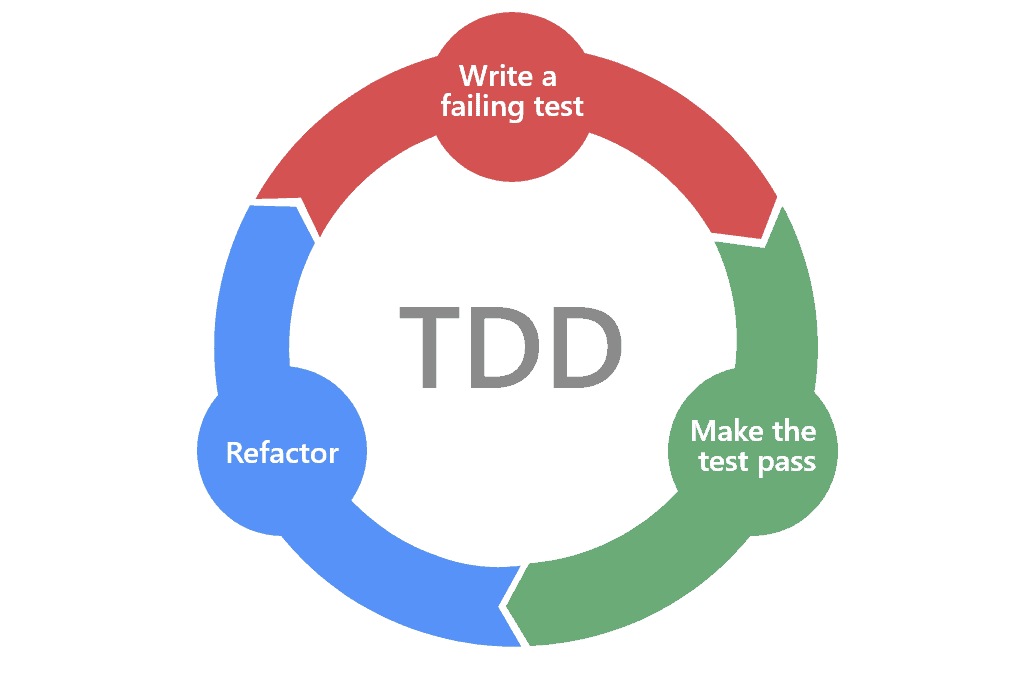
\includegraphics[width=10cm]{images/tdd.png}
    \caption{Zasada Red-Green-Refactor}
    \label{fig:redgreen}
\end{figure}

\subsubsection{Metodyki pisania testów}
\par Najpopularniejsze obecnie są dwie metody pisania testów: 
\begin{itemize}
    \item TDD - Test Driven Development - zaproponowana została przez Kenta Becka w 2002 roku. \cite{TestDrivenDevelopment} Zakłada, że testy będą napędzały tworzenie projektu i stały u jego podstawy. 
    \par Pierwszym krokiem przy implementacji nowej funkcji w naszym projekcie powinno być napisanie samego testu, który oczywiście na początku nie powiedzie się, ponieważ kod, który ma on testować nie został jeszcze napisany. Po napisaniu testu przechodzi się do pisania kodu, który w jak najłatwiejszy sposób będzie w stanie zaliczyć napisany przez nas test. Ostatnim krokiem tego cyklu jest refactoring kodu, polepszający jego jakość samą w sobie, ale bez zmieniania jego funkcjonalności, tak aby spełniał on oczekiwane standardy.
    Takie podejście pozwala na tworzenie dobrze zaprojektowanego kodu, który jest w całości pokryty testami, co owocuje w przyszłości, kiedy konieczne jest wprowadzanie zmian w bazie kodu.
    
    Pozwala to również na wymuszenie na osobach piszących kod, aby był on dobrze przemyślany. Konieczność napisania testu przed implementacją funkcjonalności wymusza na programiście, aby zastanowił się dogłębniej jak ma wyglądać struktura jego kodu oraz co chce on osiągnąć implementując daną klasę. 
    
    Podejście TDD zapewnia więc wiele zalet, ale nie jest ono oczywiście całkowicie pozbawione wad. Jedną z nich jest konieczność nauczenia programistów tej metodologii w przypadku jeśli wcześniej nie mieli z nią do czynienia. Główną wadą jest jednak znacznie zwiększony narzut czasowy na pisanie testów wynikający z wykorzystania TDD. Duże pokrycie kodu testami zajmuje programistom zwykle znacznie więcej czasu niż podczas standardowego implementowania funkcjonalności, a następnie napisania testów dla wybranych wedle uznania fragmentów kodu. Zainwestowany jednak w ten sposób czas zwraca się w późniejszych fazach projektu, jeśli okazuje się, że konieczna jest jakaś zmiana w strukturze kodu. Najwięcej czasu oszczędza się w porównaniu do standardowych metod pisania kodu na poprawianiu błędów działania programu. Wszystkie błędy poprawiane są na bieżąco, nie ma możliwości implementacji funkcjonalności bez poprawnego spełnienia napisanego wcześniej testu. W przypadku gdy taki test nie został nigdy napisany lub gdy błąd danej funkcji wynika z innego fragmentu kodu, jego znalezienie i naprawa może pochłonąć dużo czasu pracy programisty. 
    
    \item BDD - Behavior Driven Development - metodologia zaproponowana przez Dana Northa w 2006 roku \cite{BehaviourDrivenDevelopment}. Zakłada ona zaangażowanie w tworzenie oprogramowania osób nietechnicznych - analityków oraz klientów dla których oprogramowanie jest tworzone. Pozwala to na lepsze określenie kierunku, w którym zmierza rozwój aplikacji oraz pozwala na uniknięcie nieporozumień dotyczących projektu pomiędzy programistami, a osobami, które mają być odbiorcami programu. 
    \par Pierwszym krokiem przy tworzeniu nowej funkcjonalności jest zdefiniowanie przez zespół biorący udział w tworzeniu programu tak zwanych "User Stories". 
    Tworzone są one według zasady "Given - When - Then (Zakładając - Gdy - Wtedy)". Można w ten sposób łatwo opisać testy, które każdy będzie w stanie zrozumieć, a następnie zaimplementować przy użyciu odpowiedniego frameworka, np. JBehave dla Java lub Behave dla Pythona. 
    
    \begin{lstlisting}[caption={Przykładowe User Story}]
User Story: Spend points in game

As a game user
In order to get a spell
I want to spend my spell points

Given that I have 5 spell points available
When I spend 2 spell points on a spell
Then I should have 3 spell points and a new spell

    \end{lstlisting}
\end{itemize}

\subsection{Testy integracyjne}
Podczas omawiania testów jednostkowych duża uwaga została nałożona na konieczność odizolowania takiego testu od reszty kodu oraz innych zależności zewnętrznych. Testy integracyjne z kolei skupiają się właśnie na sprawdzeniu czy nasz kod działa poprawnie z innymi jego fragmentami oraz zależnościami zewnętrznymi, takimi jak komunikacja z bazami danych, API działającym na serwerze lub plikami na dysku. 

Głównym wyzwaniem przy pracy z testami integracyjnymi jest zwykle znalezienie przyczyny problemu, przez który testy nie mogą się powieść. W testach jednostkowych - o ile były poprawnie napisane nie stanowi to zwykle dużego problemu, z kolei testując więcej elementów znalezienie przyczyny problemu może wymagać więcej wysiłku. Problem może wynikać między innymi z implementacji danych systemów przez różne osoby w różnym czasie, kiedy mogły zmienić się wymagania i oczekiwania od projektu.

Należy pamiętać, że testy integracyjne trwają znacznie dłużej niż jednostkowe, z reguły będzie ich także znacznie mniej, z uwagi na to, że takich zależności będzie mniej niż najmniejszych możliwych do przetestowania fragmentów kodu. Z tego powodu warto rozważyć w projekcie zmianę strategii testowania w porównaniu z testami jednostkowymi. Tamte można zwykle wykonywać zarówno przy każdej kompilacji programu oraz przy publikowaniu zmian w repozytorium kodu. Przy testach integracyjnych można rozważyć wykonywanie ich tylko przy wysyłaniu do repozytorium do gałęzi deweloperskiej lub produkcyjnej. 

\subsubsection{White Box Testing}
Pojęcie White Box Testing ma odniesienie zarówno do testów jednostkowych oraz integracyjnych. Jest to technika testowania oprogramowania, w której znana jest wewnętrzna struktura programu oraz sposób jego działania. Powoduje to, że osoby testujące projekt muszą mieć zarówno podstawową wiedzę dotyczącą programowania w języku w jakim został napisany program, ale i wiedzę dotyczącą projektu samego w sobie. 

Testy te przeprowadzane są zwykle gdy projekt jest w zaawansowanym stopniu rozwoju. Podczas takich testów sprawdzane jest między innymi czy wywołane zostają wszystkie wymagane metody, czy możliwe jest wykonanie wszystkich stworzonych gałęzi w pętlach warunkowych, a także bezpieczeństwo aplikacji, z którego może wynikać ryzyko utraty lub wycieku danych. 

\subsection{Testy end-to-end}
Testy e2e są zwykle jednym z ostatnich etapów testowania oprogramowania. W przeciwieństwie do poprzednich rodzajów nie skupiają się one na testowaniu małych fragmentów kodu lub powiązań pomiędzy różnymi zależnościami, a na testowaniu całości aplikacji. 
Sprawdzane jest podczas nich czy aplikacja spełnia wszystkie wymagania klienta, które opisane zostały w specyfikacji, wszystkie połączenia z zależnościami zewnętrznymi oraz działanie na określonych środowiskach. Dopiero takie pełne sprawdzenie działania pozwala na bezpieczne oddanie aplikacji w ręce klienta lub użycie jej przez nas w środowisku produkcyjnym. 

Testerzy sprawdzają czy możliwe jest poprawne używanie wszystkich dostępnych elementów interfejsu, funkcji użytkowych i czy da się poprawnie zrealizować wszystkie założone scenariusze wykorzystania programu. Wszystkie wykryte problemy zgłaszane są deweloperom, którzy analizują wyniki testów, a następnie wprowadzają zmiany w kodzie, które przechodzą ponownie przez testy jednostkowe, integracyjne oraz kolejny raz end-to-end.

\subsubsection{Black Box Testing}
Z terminem testowania end-to-end często łączone jest pojęcie Black Box Testing. W przeciwieństwo do testów White Box, osoba wykonująca testy nie posiada wiedzy na temat struktury programu oraz szczegółów w jaki sposób on działa. 

Testerami mogą tutaj być osoby nieposiadające wiedzy programistycznej, ani dotyczącej projektu. Ich zadaniem jest dostarczanie danych wejściowych i weryfikacja czy dane zwracane przez program odpowiadają oczekiwaniom.

\subsection{Udział różnych poziomów testowania}
\begin{figure}[htbp]
    \centering
    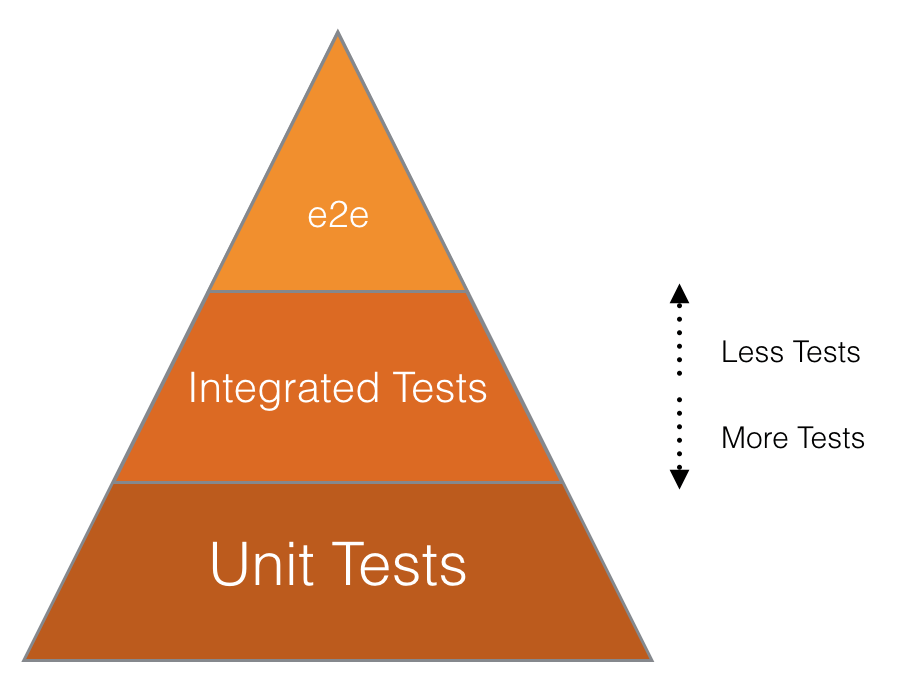
\includegraphics[width=10cm]{images/testing_triangle.png}
    \caption{Piramida testów}
    \label{fig:testing}
\end{figure}

Jak nie trudno było się domyślić znaczną większość testów w kodach programów stanowią testy jednostkowe. Wynika to z dużej popularności metodyki testowania TDD oraz coraz częstszego zauważania przez programistów korzyści wynikających z wykonywania testów. Naturalnym rezultatem chęci zwiększenia procentowego pokrycia kodu testami jest tworzenie większej liczby testów jednostkowych.

Według statystyk opublikowanych przez serwis GitLab\cite{GitLabTesting} testy jednostkowe stanowią na dzień 01.05.2019 71\% wszystkich testów odnalezionych w kodzie. Testy integracyjne oraz White Box pozostają umiarkowanie popularne, natomiast obecność testów Black Box wynosi jedynie 0.17\%.

\begin{center}
\begin{tabular}{ |c|c| } 
 \hline
 Poziom testowania & Ilość testów  \\ 
  \hline
 Testy Black-box (e2e)  & 99 (0.17\%) \\ 
 Testy White-box  & 6440 (10.9\%) \\ 
 Testy integracyjne & 10,577 (17.9\%)  \\ 
 Testy jednostkowe & 41,809 (71\%)  \\ 
 \hline
\end{tabular}
\end{center}

Biorąc pod uwagę, że znaczną większość przeprowadzanych testów stanowią w kodzie testy jednostkowe oraz integracyjne ważne okazują się metody ich automatyzacji. Wykorzystana do tego zostanie praktyka CI - Continuous Integration. 

\subsection{Rola CI w testach}
Zaczynając myślenie o Continuous Integration trzeba najpierw zrozumieć, że nie jest możliwe jednoznaczne zdefiniowanie jak taka ciągła integracja będzie wyglądać w każdym projekcie. Nasze oczekiwania i wymagania od takiej integracji często będą zależne od rodzaju projektu przy którym pracujemy, struktury firmy, wymagań biznesowych od klienta, od faktu czy nasz projekt działa na zasadzie Open Source. Wynika to z faktu, że obecnie ciągła integracja wykorzystywana jest znacznie szerzej niż tylko przeprowadzanie testów w kodzie. 

Ciągła integracja ma pozwolić zespołowi deweloperów na łatwiejsze i bezpieczniejsze tworzenie kodu, podczas którego nie będzie konieczności poświęcania dużej ilości czasu na zarządzanie bazą kodu oraz rozwiązywanie problemów, które wynikają z jednego błędu, a który dotyka dużej części systemu. W praktyce głównym celem do którego dążymy implementując ciągłą integrację jest stworzenie systemu, który po każdym dodaniu kodu do repozytorium będzie uruchamiać wszystkie wyznaczone przez nas testy - zwykle jednostkowe i integracyjne oraz sprawdzi czy dodawany kod spełnia wszystkie narzucone mu wymagania. 

Warto pamiętać, że sam fakt korzystania z systemu zarządzania wersjami, jakim jest git, można potraktować jako ważny element ciągłej integracji. Bez wykorzystania jednego repozytorium kodu dla całego projektu, zarządzanie nim byłoby znacznie bardziej czasochłonne, skomplikowane, a co za tym idzie podatne na powstawanie błędów i różnorakich problemów. Tworzenie projektów przy udziale więcej niż kilku osób mogłoby wymagać więcej czasu na ręczne wysyłanie i łączenie kodu niż samo jego pisanie. 

Jedną z praktyk wykorzystywaną w CI jest częste publikowanie naszych zmian w kodzie do repozytorium. Najczęściej będzie to przynajmniej jeden raz na każdy dzień pracy programisty. Podejście takie sprawia, że łatwiej wykryć jest ewentualne problemy, które mogą pojawić się po naszych zmianach. W przypadku gdy publikowana jest większa ilość kodu, znalezienie przyczyny problemu może byś skomplikowane. Dodatkowo częste publikowanie zmian oznacza, że łatwiej jest połączyć kod pisany w jednym miejscu w pliku przez kilku różnych programistów w procesie "mergowania" zmian. 

Częste publikowanie zmian powoduje też, że kod można łatwiej ze sobą połączyć, w zasadzie jest on zwykle łączony z resztą kodu przez cały swój cykl życia. Aby umożliwić taką sytuację developerzy stają się często pracować tylko na jednej gałęzi deweloperskiej, a gdy nie jest to możliwe wykorzystują gałęzie dedykowane danej funkcjonalności przez jak najkrótszy możliwy czas, aby móc jak najszybciej w jak największym stopniu integrować ich kod z resztą. Dodatkową zaletą szybkiej integracji nowej funkcjonalności jest umożliwienie lepszego i szybszego reagowania na ewentualne zmiany w specyfikacji lub kierunku rozwoju projektu. Stworzona funkcjonalność może być na bieżąco testowana przez osoby odpowiedzialne za tworzenie specyfikacji. W razie zmiany strategii tworzenia projektu będzie można stosunkowo szybko wprowadzić odpowiednie zmiany bez marnowania zbędnie dużej ilości czasu zespołu.

Dużą zaletą wynikającą ze stosowania ciągłej integracji jest znaczne ułatwienie skalowania. Dotyczy to zarówno skalowania projektu jako kod, ale także jako zespół programistyczny. Dobrze przetestowany i przemyślany kod ma szansę być znacznie łatwiej rozbudowywalny od takiego, który nie powstawał w wyniku stosowania dobrych praktyk programistycznych. 

Ułatwienie skalowania zespołu wynika z łatwiejszego wdrażania nowych członków do projektu, dotyczy te szczególnie osób na stanowiskach juniorskich. Kod dodawany przez takie osoby często musiał przechodzić przez recenzję od osoby na stanowisku seniora w celu upewnienia się, że spełnia on oczekiwane standardy. Wykorzystanie Continuous Integration w znacznym stopniu wspomaga taki proces, poprzez wykorzystanie następujących funkcji: 

\begin{itemize}
    \item Automatyczne przeprowadzanie testów 
    
    Jest to podstawowe zadanie praktycznie każdej implementacji Continuous Integration. Zapewnia to możliwość uniknięcia regresji podczas dodawania nowego kodu oraz utrzymywania starego. 
    Platforma na której dokonujemy integracji może zostać skonfigurowana, aby nie pozwolić na dodanie do repozytorium kodu, który nie przejdzie określonych testów. Zwykle będą to wszystkie testy jednostkowe, integracyjne oraz wybrane testy e2e, aktywowane w kodzie przez specjalne flagi, oznaczające elementy projektu, które powinny być poprawnie zaimplementowane. 
    \item Sprawdzanie pokrycia kodu testami
    
    Pokrycie testami ( code coverage ) to bardzo ważna statystyka. Wyraża ona w punktach procentowych jak duża część wyrażeń w naszym projekcie jest testowana. Statystykę tę można wykorzystać, w razie gdyby ktoś próbował dodać do repozytorium nieprzetestowany kod. Oczywiście możliwe jest obejście takiego sprawdzenia poprzez napisanie niepoprawnego testu, który nie wnosi żadnej wartości, jednak w dobrych zespołach programistycznych statystyka jest pomocna jeśli chcemy zachować dobrą jakość pisanego kodu. Istnieją opinie, że pokrycie testami powinno wynosić 100\%, jednak zwykle spotykają się one z opinią, że nie przyniesie to wymiernych rezultatów, ponieważ nawet wtedy w programie mogą znaleźć się błędy logiczne, których nie da się wykryć automatycznymi testami. Zwykle przyjmuje się wartości 80\% - 95\% za odpowiednie przy szacowaniu wymaganego pokrycia kodu. Znalezienie odpowiedniej pracy dla naszego projektu wymaga doświadczenia, znajomości zespołu i zrozumienia wymagań jakie stawia przed nami projekt.
    \item Linting kodu
    
    Lintingiem kodu nazywamy wykorzystanie narzędzie do statycznej analizy kodu. Jego zadaniem w przypadku wykorzystania do ciągłej integracji jest sprawdzanie czy kod, który próbujemy dodać odpowiada standardom wykorzystywanym w projekcie. Może to dotyczyć między innymi tego czy nawiasy otwieramy w nowej linii, konwencji tworzenia nazw zmiennych ( wykorzystanie camelCase, PascalCase, podkreślenia ), definiowania argumentów funkcji w wielu liniach. Z pozoru rola lintingu wydaje się mała, a nawet zbędna, jednakże w dużych projektach, przy których pracuje wiele osób o różnych preferencjach ważne jest tworzenie kodu, który jest jednolity stylistycznie, aby był on spójny i łatwy w czytaniu dla osób, które nie mają z nim dużego doświadczenia.
    \item Integracja z kanałem komunikacji
    
    Wykorzystanie Continuous Integration umożliwia synchronizację naszego repozytorium z wykorzystywanym w projekcie kanałem komunikacyjnym. Obecnie najpopularniejszym wykorzystywanym w profesjonalnych projektach jest Slack, a w projektach tworzonych przez społeczność często także Discord. Integracja taka umożliwia nam otrzymywanie na naszym kanale powiadomień dotyczących repozytorium. Możemy skonfigurować je aby otrzymywać je za każdym razem kiedy nie uda się wykonać testu przy próbie dodania kodu. Możliwe będzie wtedy szybsze naprawienie problemu, jeśli powiadomienie otrzymają odpowiednie osoby i będą mogły szybciej zareagować. Powiadomienia możemy wysyłać też przy poprawnym przejściu testów, co może się przydać jeśli wykonujemy skomplikowane testy, których wykonanie zajmuje więcej czasu. 
\end{itemize}

\begin{figure}[htbp]
    \centering
    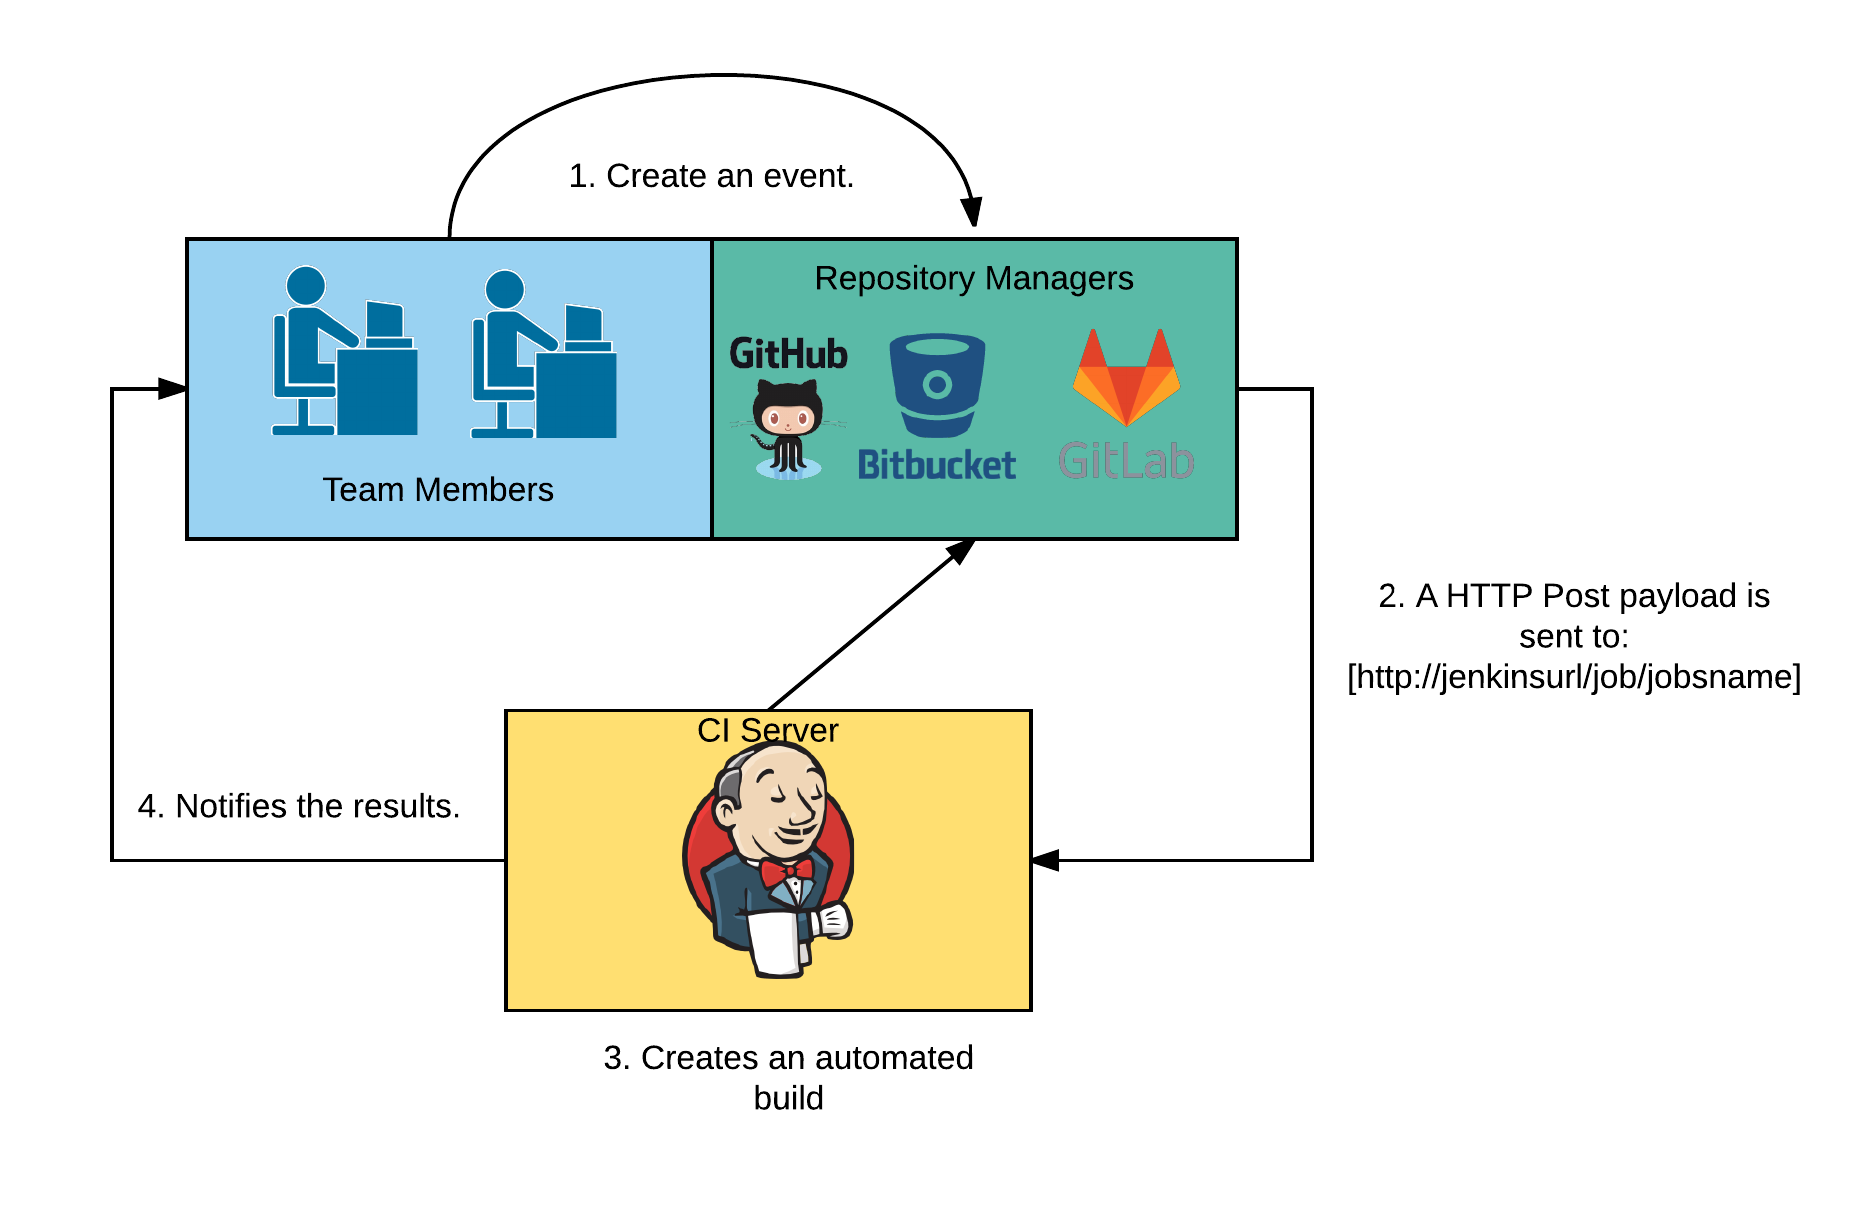
\includegraphics[width=13cm]{images/ci_flow.png}
    \caption{Schemat działania CI, źródło: medium.com/@automationdiscovery}
    \label{fig:ciflow}
\end{figure}

\subsubsection{Wykrywanie błędów bezpieczeństwa}
Dużą korzyścią wynikającą z ciągłej integracji jest możliwość otrzymywania powiadomień dotyczących problemów z bezpieczeństwem w naszym projekcie. Mogą one dotyczyć zarówno błędów wykrytych w wykorzystywanych bibliotekach zewnętrznych jak i przykładowo prywatnych kluczy API, których nie powinniśmy udostępniać publicznie w repozytorium. 

W przypadku wykorzystania platformy GitHub jako repozytorium otrzymujemy alerty o błędach bezpieczeństwa w bibliotekach bez konieczności jakiejkolwiek konfiguracji. 

\begin{figure}[htbp]
    \centering
    
\includegraphics[width=10cm]{images/GitHubAlert.png}
    \caption{Powiadomienie bezpieczeństwa z serwisu GitHub, źródło: własne}
    \label{fig:githubalert}
\end{figure}

Dostępne są także alternatywne serwisy monitorujące repozytoria. Wykorzystanie ich może być konieczne w przypadku projektów komercyjnych, których repozytoria nie są publicznie dostępne. Jednym z popularniejszych jest GitGuardian, który umożliwi nam indywidualne dostosowanie go do potrzeb naszego projektu. 

\begin{figure}[htbp]
    \centering
    
\includegraphics[width=13cm]{images/GitGuardian.png}
    \caption{Powiadomienie bezpieczeństwa z serwisu GitGuardian, źródło: własne}
    \label{fig:gitguardian}
\end{figure}

\subsection{Przykład CI w GitHub Actions}
W celu przetestowania działania różnych funkcjonalności CI do testowania kodu wykorzystamy język python, platformę GitHub oraz oferowaną przez nią usługę GitHub Actions, której działanie zostało już opisane we wcześniejszych częściach pracy.

Nasz projekt spełniać ma następujące założenia: 
\begin{itemize}
    \item Automatycznie wykonywane są wszystkie testy. Do napisania ich wykorzystany zostanie framework pytest. Innym popularnym wyborem dla języka python jest framework unittest. Wybór padł na ten pierwszy ponieważ proste testy można w nim napisać w nieco łatwiejszy sposób, przeszukuje on automatycznie całą bazę kodu w poszukiwaniu testów i umożliwia szybkie uruchomienie ich jedną komendą. Ponadto większość testów pisanych dla unittest zadziała prawidłowo w pytest.
    \item Automatycznie wykonywane jest sprawdzenie pokrycia testami naszego kodu. Wykorzystana zostanie do tego platforma Codecov, która została wybrana z uwagi na łatwą możliwość połączenia z GitHub Actions
    \item Projekt zintegrowany jest z kanałem Slack, na który wysyłane są powiadomienia o działaniach w repozytorium. Slack został wybrany z uwagi na możliwość łatwej integracji z GitHub Actions oraz swoją popularność przy wykorzystaniu w projektach informatycznych. 
\end{itemize}

Pierwszym krokiem było stworzenie repozytorium z kodem i przygotowanymi dla niego testami. 

\begin{figure}[htbp]
    \centering
    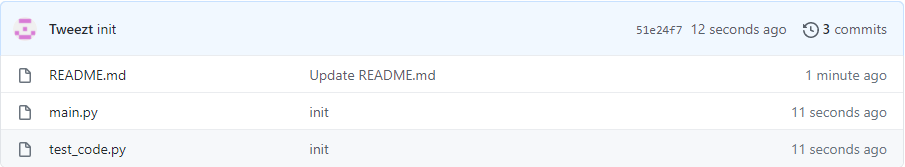
\includegraphics[width=13cm]{images/testingCI1.png}
    \caption{Stworzone repozytorium z przykładowym kodem, źródło: własne}
    \label{fig:ci1}
\end{figure}

\subsubsection{Automatyczne przeprowadzanie testów}
W celu automatycznego wykonywania testów po każdym dodaniu kodu do repozytorium konieczne jest stworzenie tak zwanego workflow. Szczegółowy opis tego zagadnienia został przedstawiony w rozdziale 4.2. 

\begin{lstlisting}[caption={plik main.yaml zawierający workflow automatycznie przeprowadzający testy}]
name: CI
on:
  push:
    branches: [ main ]
  pull_request:
    branches: [ main ]

jobs:
  runtests:
    runs-on: ubuntu-latest

    steps:
      - uses: actions/checkout@v2

      - name: Setup Python
        uses: actions/setup-python@v2.2.1
        with: 
          python-version: 3.8 

      - name: Run tests
        run: |
          pip install pytest
          pytest
\end{lstlisting}

Wykorzystany został w nim system operacyjny Ubuntu w najnowszej wersji oraz język python w wersji 3.8, ponieważ na takiej wersji były przeprowadzane testy lokalne. Samo wykonanie testów odbywa się w dwóch ostatnich liniach. Najpierw instalowana jest biblioteka pytest, a następnie jednym poleceniem uruchamiane są wszystkie zaimplementowane w kodzie testy. 

\begin{figure}[htbp]
    \centering
    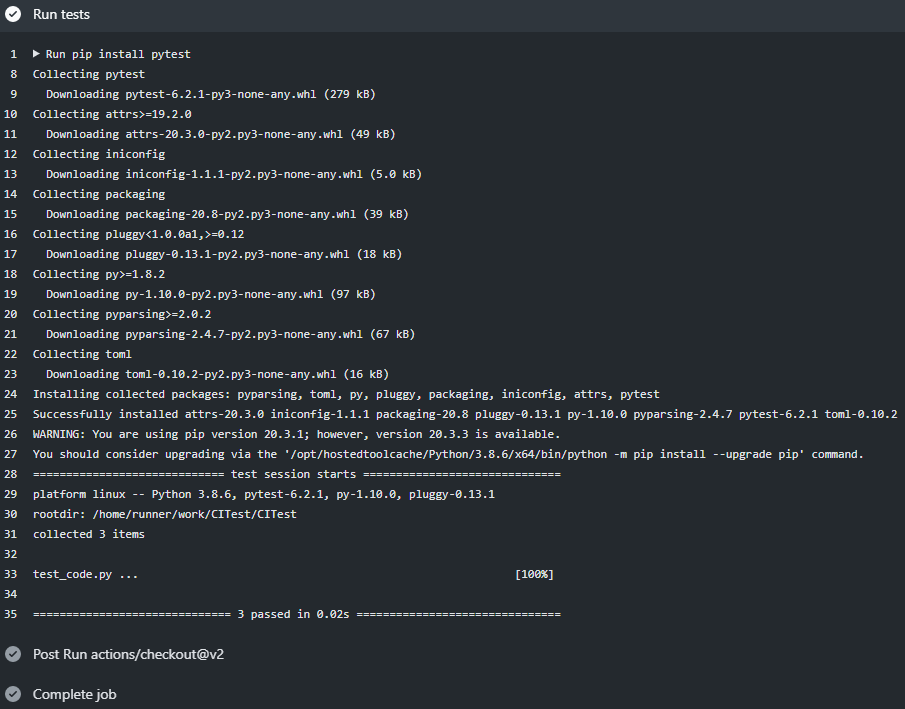
\includegraphics[width=11cm]{images/testingCI3.png}
    \caption{Wynik uruchomionej akcji z testami, źródło: własne}
    \label{fig:ci3}
\end{figure}

Po przejściu do zakładki Actions, można zobaczyć, że testy wykonane zostały poprawnie. 
Po celowym sprawieniu, że test jednostkowy nie powodzi się i opublikowaniu zmian w repozytorium można zobaczyć że jesteśmy o tym informowani w zakładce Actions oraz nad listą plików w repozytorium. 

\begin{figure}[htbp]
    \centering
    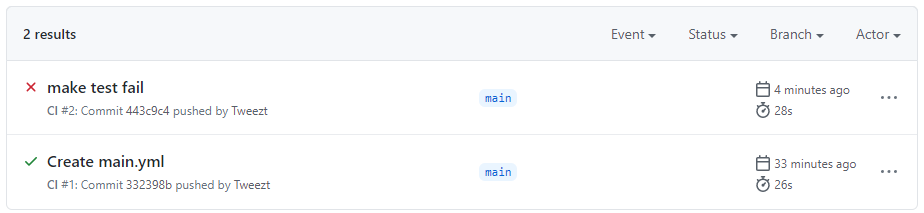
\includegraphics[width=11cm]{images/testingCI4.png}
    \caption{Negatywny wynik testu w zakładce Actions, źródło: własne}
    \label{fig:ci4}
\end{figure}

\begin{figure}[htbp]
    \centering
    
\includegraphics[width=7cm]{images/testingCI5.png}
    \caption{Negatywny wynik testu nad listą plików, źródło: własne}
    \label{fig:ci5}
\end{figure}

\subsubsection{Integracja z serwisem Codecov}
Pierwszym krokiem do przeprowadzenia integracji z serwisem Codecov było zalogowanie się tam przy pomocy konta GitHub, na którym znajduje się repozytorium z projektem. Po udanym zalogowaniu konieczne było pobranie klucza CODECOV\_TOKEN, który należy umieścić w odpowiednim miejscu w ustawieniach repozytorium. Kolejnym krokiem było utworzenie kolejnego pliku .yaml odpowiedzialnego za uruchamianie nowego workflow. 

\begin{lstlisting}[caption={plik coverage.yaml zawierający workflow automatycznie sprawdzający pokrycie testami}]
name: coverage testing
on:
  push:
    branches: [ main ]
    
jobs:
  runtests:
    runs-on: ubuntu-latest
    steps:
      - uses: actions/checkout@v2

      - name: Setup Python
        uses: actions/setup-python@v2.2.1
        with: 
          python-version: 3.8 
      - name: Generate coverage report
        run: |
          pip install pytest
          pip install pytest-cov
          coverage run test_code.py
          coverage report
          coverage xml
      - name: Upload  to Codecov
        uses: codecov/codecov-action@v1
        with:
          token: ${{ secrets.CODECOV_TOKEN }}
          file: ./coverage.xml
          flags: unittests
\end{lstlisting}

Wykorzystywana jest tutaj akcja codecov-action, która pozwala nam w łatwy sposób automatycznie wysłać nasz raport do serwisu. Po prawidłowym wykonaniu wszystkich operacji możemy zobaczyć nasze pokrycie testami w serwisie Codecov.io. 

\begin{figure}[htbp]
    \centering
    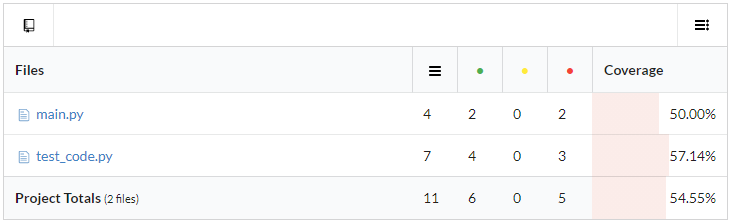
\includegraphics[width=12cm]{images/testingCI6.png}
    \caption{Raport pokrycia kodu testami, źródło: własne}
    \label{fig:ci6}
\end{figure}

\subsubsection{Integracja z kanałem Slack}
Integrację z kanałem Slack można przeprowadzić w sposób analogiczny do integracji z serwisem Codecov, pomocne są tutaj Akcje dystarczone przez te serwisy, które powodują, że konieczna konfiguracja sprowadza się do podania odpowiednich kluczy dostępu. Z tego powodu wykorzystamy odmienne podejście, aby sprawdzić jak można dokonać takiej integracji od strony Slacka. 

Pierwszym krokiem było dodanie aplikacji GitHub do naszego kanału Slack. Można ją znaleźć w galerii aplikacji, dostępnej pod adresem \url{citestingworkspace.slack.com/apps}. Po poprawnym uwierzytelnieniu konta należy wybrać, do których kanałów chcemy dać aplikacji dostęp. 

\begin{figure}[htbp]
    \centering
    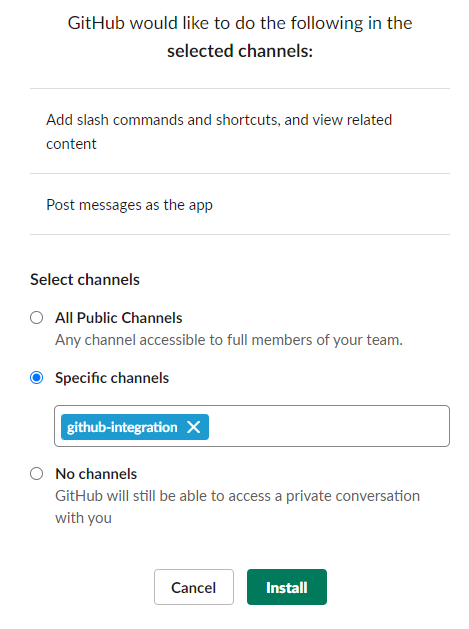
\includegraphics[width=5cm]{images/testingCI7.png}
    \caption{Nadanie aplikacji GitHub uprawnień do korzystania z kanałów, źródło: własne}
    \label{fig:ci7}
\end{figure}
Ostatnim krokiem jak wskazanie aplikacji, z którym repozytorium w serwisie GitHub chcemy ją zintegrować. Odbywa się to poprzez polecenie 
\begin{lstlisting}[caption={Polecenie pozwalające połączyć aplikację GitHub z repozytorium}]
/github subscribe owner/repository
\end{lstlisting}

gdzie owner to nazwa konta, a repository to nazwa naszego repozytorium. 

Po wykonaniu wszystkich kroków i udostępnieniu nowej zmiany w repozytorium możemy zobaczyć powiadomienie wysłane nam przez nowo zainstalowaną aplikację. 

\begin{figure}[htbp]
    \centering
    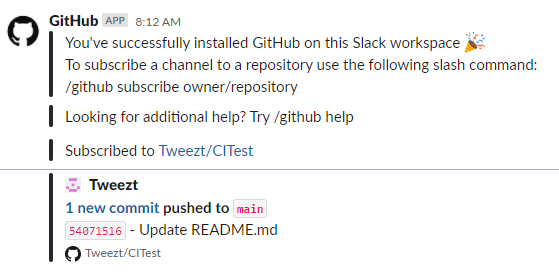
\includegraphics[width=12cm]{images/testingCI9.png}
    \caption{Powiadomienie o nowych zmianach w kodzie w repozytorium, źródło: własne}
    \label{fig:ci9}
\end{figure}

Po wykonaniu wszystkich tych czynności udało nam się stworzyć repozytorium, które dzięki wykorzystaniu ciągłej integracji pozwala na sprawne przeprowadzanie testów, analizę pokrycia nimi kodu oraz umożliwia automatyczne informowanie członków zespołu o zmianach w kodzie. 


\section{Podsumowanie i wnioski}
Pisząc naszą pracę chcieliśmy zgromadzić jak największą ilość wiedzy oraz dobrych praktyk, dotyczących nowoczesnych metod tworzenia oprogramowania. Z tego też powodu pracę otworzyliśmy rozdziałem wprowadzającym, w którym przybliżyliśmy jak istotną rolę w dzisiejszym przemyśle informatycznym odgrywa automatyzacja procesów. Dużą część naszej pracy stanowi teoria, ponieważ uważamy, że zrozumienie idei jest pierwszym i najistotniejszym krokiem, dzięki któremu nasza praca przy automatyzacji będzie skuteczna.

Automatyzacja jest stosowana powszechnie w praktycznie każdym zespole programistycznym. Z powodu jej powszechności i dostępności materiałów do nauki coraz częściej implementowana jest też przez programistów w prywatnych projektach, ponieważ widzą oni wartość dodaną, która ona wnosi. 

My również zauważyliśmy takie korzyści, dlatego podczas pracy zdecydowaliśmy się na implementację zasady CI/CD, dzięki której nasz plik \LaTeX po opublikowaniu zmian w repozytorium automatycznie budował się i publikował w formacie .pdf na stronie internetowej w formie łatwej do czytania. 

\begin{figure}[htbp]
    \centering
    
\includegraphics[width=12cm]{images/podsumowanie.png}
    \caption{Budowanie nowych wersji naszej pracy, źródło: własne}
    \label{fig:podsumowanie}
\end{figure}

Podejście CI/CD pozwala programistom na efektywne wykonywanie swoich obowiązków. Eliminowane są zbędne przestoje w pracy, problemy wynikające z regresji w kodzie, a same nowe funkcjonalności publikowane są szybciej. Ciągłe testowanie wzmacnia pewność siebie programisty, nie musi się on martwić, że jego zmiany spowodują problemy dla reszty członków zespołu, w najgorszym wypadku jego zmiany nie zostaną zaakceptowane. 

Uważamy, że temat naszej pracy można jeszcze zdecydowanie pogłębić. Możliwa byłaby analiza innych platform programistycznych oraz metod tworzenia oprogramowania.  Dziedzina ta bardzo szybko się rozrasta i uważamy, że warto interesować się zagadnieniami automatyzacji w programowaniu, ponieważ może się to okazać opłacalne w przyszłości.  

\begin{thebibliography}{12}

\bibitem{AgileManifesto} Kent Beck; James Grenning; Robert C. Martin; Mike Beedle; Jim Highsmith; Steve Mellor; Arie van Bennekum; Andrew Hunt; Ken Schwaber; Alistair Cockburn; Ron Jeffries; Jeff Sutherland; Ward Cunningham; Jon Kern; Dave Thomas; Martin Fowler; Brian Marick (2001). "Principles behind the Agile Manifesto"
\bibitem{DevOpsBook} Bass, Len; Weber, Ingo; Zhu, Liming (2015). DevOps: A Software Architect's Perspective
\bibitem{TravisCI} Mathias Meyer (2015)  "How We Improved the Installation and Update Experience for Travis CI Enterprise" \url{https://blog.travis-ci.com/2015-06-19-how-we-improved-travis-ci-installation/}
\bibitem{UnitOpinions} kayis (2018)"What are the alternatives to unit tests?" \url{https://dev.to/kayis/what-are-the-alternatives-to-unit-tests-2jii}
\bibitem{UnitResults} kayis (2018) "The Dev.to-Community's Opinion about Unit-Tests" \url{https://dev.to/kayis/the-devtos-opinion-about-unit-tests-1md2}
\bibitem{UnitDefinition} Roy Osherove (2011) "Unit Test - Definition" \url{https://www.artofunittesting.com/definition-of-a-unit-test/}
\bibitem{TestDrivenDevelopment} Kent Beck (2002). "Test Driven Development: By Example"
\bibitem{BehaviourDrivenDevelopment} Dan North (marzec 2006). Magazyn "Better Software" \url{https://dannorth.net/introducing-bdd/}
\bibitem{RegressionTesting} GURU99, "What is Regression Testing? Definition, Test Cases (Example)" \url{https://www.guru99.com/regression-testing.html}
\bibitem{GitLabTesting} GitLab, Dokumentacja "Testing levels" \url{https://docs.gitlab.com/ee/development/testing\_guide/testing\_levels.html}
\bibitem{TravisCI} Mathias Meyer (2015)  "How We Improved the Installation and Update Experience for Travis CI Enterprise" https://blog.travis-ci.com/2015-06-19-how-we-improved-travis-ci-installation/
\bibitem{GatsbyJSWordpress} Praca zbiorcza twórców GatsbyJS "Sourcing from WordPress" https://www.gatsbyjs.com/docs/sourcing-from-wordpress/
\bibitem{GithubActionsDoc} Autor nieznany "GitHub Actions Reference" https://docs.github.com/en/free-pro-team@latest/actions/reference
\bibitem{Computing} Paul E. Ceruzzi "A History of Modern Computing"
\bibitem{Computer Systems} Randal Bryant "Computer Systems: A Programmer's Perspective"
\bibitem{Docker} James Turnbull "The Docker Book: Containerization Is the New Virtualization"
\bibitem{PragmaticProgrammer} Andrew Hunt, David Thomas "The Pragmatic Programmer"
\bibitem{DevOps} Gene Kim, Kevin Behr "The Phoenix Project: A Novel about IT, DevOps, and Helping Your Business Win"
\bibitem{Jenkins} John Smart "Jenkins: The Definitive Guide"

\end{thebibliography}
\end{document}
